\RequirePackage[l2tabu, orthodox]{nag}
\documentclass[10pt]{book}

% Language support
\usepackage[spanish, english]{babel}

% Thesis format
\usepackage[paperheight=24cm, paperwidth=17cm]{geometry}

% Graphics support
\usepackage{graphicx}
\graphicspath{{figures/}}

% Useful math features
\usepackage{amssymb}
\usepackage{amsmath}
\usepackage{bm}

% Alter geometry of the page headers:
\usepackage{fancyhdr} 

% Packages used by Pygments for highlighting source code
\usepackage{fancyvrb}
\usepackage{color}
\usepackage[mathletters]{ucs}
\usepackage[utf8x]{inputenc}
\input{pygments_preamble}

% Fancy tables
\usepackage{booktabs}

% Citations are numbered, sorted and consequtive lists compressed:
\usepackage[numbers, compress, sort]{natbib}

% Allow appendices in chapters:
\usepackage[toc]{appendix}

% Sans serif for section names:
\usepackage{sectsty}
\allsectionsfont{\sffamily}
\chapterfont{\LARGE \sffamily}

% Setting header height:
\headheight 14pt

% Setting text size:
\setlength{\textwidth}{12.3cm}
\setlength{\textheight}{18.5cm}

% Setting margins:
\setlength{\oddsidemargin}{-1in}
\setlength{\evensidemargin}{-1in}
\setlength{\topmargin}{-1in}
\addtolength{\oddsidemargin}{2.5cm}
\addtolength{\evensidemargin}{2.2cm}
\addtolength{\topmargin}{1.8cm}

% Parameters for fancy headers:
\pagestyle{fancyplain}
\renewcommand{\chaptermark}[1]{\markboth{\chaptername\ \thechapter.\ #1}{}}
\renewcommand{\sectionmark}[1]{\markright{\thesection\ #1}}
\lhead[\fancyplain{}{\thepage}]{\fancyplain{}{\rightmark}}
\rhead[\fancyplain{}{\leftmark}]{\fancyplain{}{\thepage}}
\cfoot{}

% Alter some LaTeX defaults for better treatment of figures.  Taken from
% http://mintaka.sdsu.edu/GF/bibliog/latex/floats.html
\renewcommand{\topfraction}{0.9}    % max fraction of floats at top
\renewcommand{\bottomfraction}{0.8} % max fraction of floats at bottom
\renewcommand{\textfraction}{0.1}   % allow minimal text w. figs

% Hyphenation:
\hyphenation{Ber-cea-nu Mar-chet-ti Ca-ru-sot-to}

% Invisible paragraphs
\newcommand{\co}[2]{#2}
\renewcommand{\paragraph}{\co}


% Abbreviations:
\newcommand*{\Lca}{\mathcal{L}}

\newcommand*{\tx}{\hat{T}_{x}}
\newcommand*{\ty}{\hat{T}_{y}}
\newcommand*{\sub}[1]{_{\text{#1}}}



\newcommand*{\la}{\langle}
\newcommand*{\ra}{\rangle}
\newcommand*{\abs}[1]{\vert #1 \vert}
\newcommand*{\bra}[1]{\langle #1 \vert}
\newcommand*{\ket}[1]{\vert #1 \rangle}
\newcommand*{\braket}[2]{\langle #1 \vert #2 \rangle}

%\newcommand*{\zb}{\bar{z}}
%\newcommand*{\e}{\epsilon}

\newcommand*{\pa}{\partial}
\newcommand*{\xv}{\bm{x}}
\newcommand*{\rv}{\bm{r}}
\newcommand*{\kv}{\bm{k}}
\newcommand*{\pv}{\bm{p}}
\newcommand*{\kop}{\hat{\bm{k}}}
\newcommand*{\vt}[1]{\mathbf{#1}}

\newcommand*{\ps}{\phi_{0}^{\star}}
\newcommand*{\p}{\phi_{0}}

% \colvec{a}{b}
\newcommand*{\colvec}[2]{
  \begin{pmatrix}
    #1\\
    #2
  \end{pmatrix}
}

% \mat{a}{b}{c}{d}
\newcommand*{\mat}[4]{
  \begin{pmatrix}
    #1 & #2\\
    #3 & #4
  \end{pmatrix}
}

\newcommand*{\etal}{\emph{et al.}}

\DeclareMathOperator{\real}{Re}
\DeclareMathOperator{\imag}{Im}
\DeclareMathOperator{\Ry}{\mathcal{R}y}

\newcommand{\noo}[1]{: \negthinspace {#1} \negthinspace :}



\begin{document}
\frontmatter

\thispagestyle{empty}

\begin{center}
{\Huge  Scattering and topological properties of \\ driven-dissipative quantum fluids\\}
\vspace{5.4cm}
{\large{TESIS DOCTORAL}}\\
\vspace{2.6cm}
{ \textsc{memoria presentada para optar al grado de \\ Doctor en Ciencias F\'{i}sicas\\
Universidad Aut\'{o}noma de Madrid\\
Departamento de F\'{i}sica Te\'{o}rica de la Materia Condensada\\
Programa de Doctorado\\
F\'{i}sica de la Materia Condensada y Nanotecnolog\'{i}a\\
viernes, 8 de julio del 2016\\
$\,$\\$\,$\\por\\$\,$\\$\,$\\}
{\LARGE{Andrei Ciprian Berceanu}}\\$\,$ \\\textsc{nacido en Bucarest, Ruman\'{i}a en 1983}}
\end{center}
\newpage

\thispagestyle{empty}
\noindent {\large\bfseries Comisi\'{o}n:}\\[2ex]
  \parbox[t]{2.8cm}{Director:\\
                  Tribunal:
}~\parbox[t]{9cm}{Prof.\ dr.\ F.\ M.\ Marchetti (UAM) \\
Prof.\ dr.\ C.\ Tejedor (UAM) \\
Prof.\ dr.\ L.\ Vi\~{n}a (UAM) \\
Dr.\ A.\ Amo (CNRS, France) \\
Dr.\ J.\ J.\ Garc\'{\i}a-Ripoll (CSIC) \\
Dr.\ T.\ Ozawa (Universit\`{a} di Trento, Italy)
}


\vfill


\noindent
\begin{otherlanguage}{spanish}
El autor agradece el apoyo financiero de FP7 ITN ``Clermont4'' y
de la European Science Foundation (ESF) a trav\'{e}s de POLATOM Grant 4914.
\end{otherlanguage}
\vspace{\baselineskip}


\noindent
The author acknowledges financial support from FP7 ITN ``Clermont4'' and
from the European Science Foundation (ESF) through POLATOM Grant 4914.
\vspace{\baselineskip}


\begin{center}
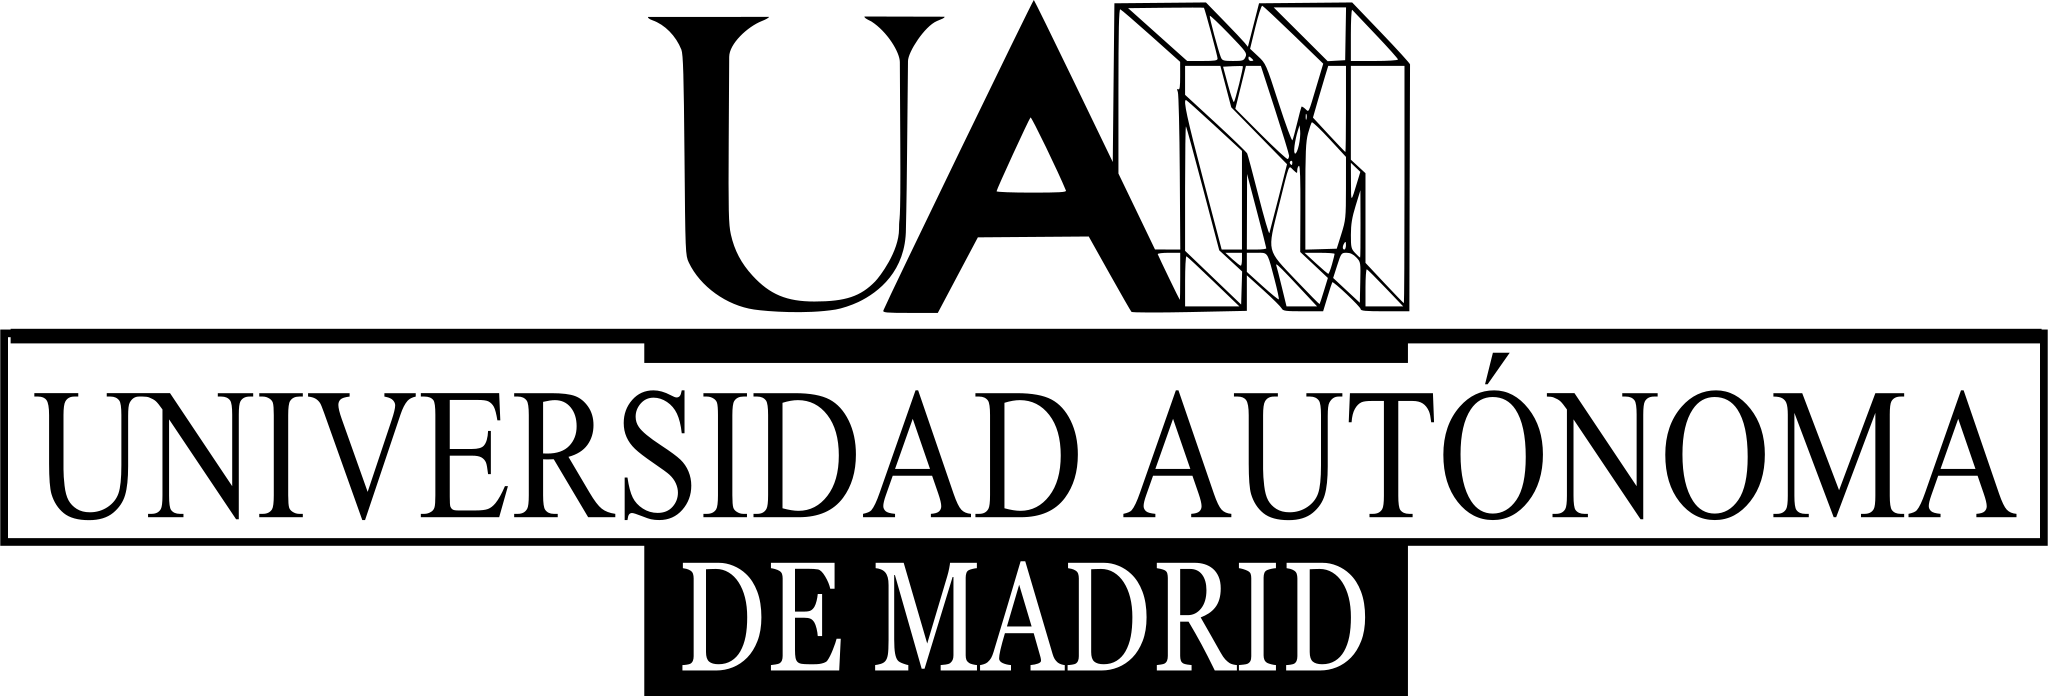
\includegraphics[width=30mm]{uam_logo}  
\end{center}


\newpage

\thispagestyle{empty}

\phantom{text}

\vspace{2cm}

\begin{flushright}
  {\em Bunicilor mei.}
\end{flushright}

\newpage

\thispagestyle{empty}

%%% Local Variables:
%%% mode: latex
%%% TeX-master: "thesis_berceanu"
%%% End:


\tableofcontents
\mainmatter

\chapter*{Resumen}
\markboth{Resumen}{}
\addcontentsline{toc}{part}{Resumen}


\textit{This short overview of the thesis work is written in Spanish as required by the Spanish Government for thesis manuscripts in a foreign language.}

\selectlanguage{spanish}
Superfluidez, la capacidad de un fluido fluya sin aparente viscosidad,
es una de las consecuencias más llamativas del colectivo coherencia
cuántica, con manifestaciones que van desde la metaestabilidad de
supercorrientes en geometrías multiplican conectados a la aparición de
vórtices cuantificados, o la existencia de una velocidad crítica para
flujo sin fricción cuando la dispersión contra un defecto. Mientras
Tradicionalmente investigado en sistemas en equilibrio, como un
líquido ${}^4$He y gases atómicos ultrafríos, los avances
experimentales en óptica no lineal, en particular en relación con
microcavity excitón-polaritonas, allanó el camino para el estudio de
superfluido relacionada fenómenos en un marco impulsado por
disipativo.

Igualmente interesante es la posibilidad de realizar las fases
topológicas de la materia, tales como el número entero o estados Hall
cuántico fraccional, fuera de los sistemas electrónicos
tradicionales. experimentos en fotónica impulsado por el resonador
disipativo matrices, en particular, ofrecen un alto grado de
controlabilidad y capacidad de ajuste, así como sin precedentes el
acceso experimental a la energía y los estados propios del espectro.

Esta tesis informa sobre los efectos hidrodinámicos, así como
topológico propiedades de los sistemas, impulsado por disipativas. En
particular, se analiza el comportamiento superfluido-como de
microcavidad excitón-polaritonas, como así como la topología de
impulso en el espacio de las matrices de resonador acoplados.

Microcavity excitón-polaritonas son cuasi-partículas resultantes de la
(mezcla de excitones ligados pares electrón-hueco) y los fotones
confinado microcavidades semiconductoras interior. Mientras que los
fluidos de polariton han sido se muestra para mostrar la coherencia
colectiva, la conexión entre el diversas manifestaciones de la
conducta superfluido es más complicado en comparación con los sistemas
de equilibrio. En este manuscipt, consideramos tanto el caso de un
solo fluido de la bomba de sólo configuración, así como la tres fluido
régimen oscilador paramétrico óptico que resulta de dispersión
paramétrica de la bomba a los estados de señal y de inversión. En
ambos casos, nos fijamos en la respuesta de los polaritonas móviles
esparciendo contra un defecto estática débil presente en el
microcavity.

Para un único líquido, evaluamos analíticamente la resistencia
ejercida por el fluido sobre el defecto. Para bajas velocidades del
fluido, la frecuencia de bombeo clasifica los espectros de excitación
colectiva en tres diferentes Categorías: lineal, de difusión similar y
con huecos. Se demuestra que tanto el casos difusivo-como lineal y
comparten un cualitativamente similar cruce de la avenida de la
subsónica a supersónica el régimen como una en función de la velocidad
del fluido, con una velocidad crítica propuesta por el velocidad del
sonido se encontró para el régimen lineal. En contraste, para gapped
espectros, nos encontramos con que la velocidad crítica excede la
velocidad de sonar. En todos los casos, se muestra que la resistencia
residual en el subcrítico régimen es causada por la naturaleza de no
equilibrio del sistema. También, muy por debajo de la velocidad
crítica, la resistencia varía linealmente con la polariton curso de la
vida, de acuerdo con estudios anteriores numéricos.

El régimen de oscilador paramétrico óptico presenta un adicional de
reto, ya que uno está tratando con tres fluidos acoplados. los la
coherencia macroscópica espontánea tras el bloqueo de fase de la
fluidos de señal y de inversión ha sido ya demostrado ser responsable
de su metaestabilidad de flujo cuantificada simultánea. Nos
encontramos con que la modulaciones generados por el defecto en cada
fluido son no sólo determinada por su anillo de dispersión asociado en
el espacio de momentos, pero cada componente muestra anillos
adicionales debido a la diafonía con los otros componentes impuestas
por no lineal y paramétrico procesos. Nos destacamos tres factores que
determinan cuál de estos anillos tiene la mayor influencia en cada
respuesta de fluido: el acoplamiento fuerza entre los tres fluidos, la
resonancia del anillo con el dispersión polariton, y los valores de
cada velocidad de grupo de fluido y vida juntos establecer en qué
medida cada uno de modulación puede propagarse del defecto. Para las
condiciones típicas de dispersión paramétrico, La bomba está en el
régimen supercrítico, por lo que la señal y la rueda loca hará mostrar
las modulaciones de la bomba, es decir, ninguno de los tres estados se
manifiesta un comportamiento superfluido. Sin embargo, la señal parece
fluir sin fricción en el estudio experimental, debido a que los tres
factores mencionado anteriormente conspiran para reducir la amplitud
de sus modulaciones debajo de los niveles detectables actualmente.

sistemas-Driven disipativas pueden mostrar fenómenos interesantes
también sin interacciones, derivados de la topología no trivial de su
energía alzacuello. En la parte final de esta tesis, presentamos un
realista propuesta de un experimento óptico que utiliza el estado de
la técnica acoplada arrays resonador. Se estudia teóricamente el
disipador impulsado modelo de Harper-Hofstadter en una red cuadrada en
presencia de un débil trampa armónica. Sin bombeo y las pérdidas, los
estados propios de esta sistema puede entenderse, bajo ciertas
aproximaciones, como impulso-espacio toroidal niveles de Landau, donde
la curvatura Berry, una propiedad geométrica de una banda de energía,
actúa como un impulso en el espacio campo magnético. Se muestra cómo
las características clave de estos estados propios pueden ser
observado en el estado de equilibrio del sistema impulsado por
disipativo bajo una impulso coherente monocromática. También se
muestra que el impulso de Landau-espacio niveles tendrían firmas
claras en las mediciones espectroscópicas en tales experimentos, y se
discuten los conocimientos adquiridos de esta manera en bandas de
energía geométricos y partículas en campos magnéticos.


\chapter*{Abstract}
\markboth{Abstract}{}
\addcontentsline{toc}{part}{Abstract}
\selectlanguage{english}

Superfluidity, the ability of a fluid to flow without apparent
viscosity, is one of the most striking consequences of collective
quantum coherence, with manifestations ranging from metastability of
supercurrents in multiply connected geometries to the appearance of
quantized vortices, or the existence of a critical velocity for
frictionless flow when scattering against a defect. While
traditionally investigated in equilibrium systems, like liquid
${}^4$He and ultracold atomic gases, experimental advances in
nonlinear optics, in particular regarding microcavity
exciton-polaritons, paved the way for studying superfluid-related
phenomena in a driven-dissipative framework.

Equally exciting is the possibility of realising topological phases of
matter, such as the integer or fractional quantum Hall states, outside
of traditional electronic systems. Photonics experiments in
driven-dissipative resonator arrays, in particular, offer a high
degree of controllability and tunability, as well as unprecedented
experimental access to the eigenstates and energy spectrum.

This thesis reports on hydrodynamic effects, as well as topological
properties, of driven-dissipative systems. In particular, we analyze
the superfluid-like behaviour of microcavity exciton-polaritons, as
well as the momentum-space topology of coupled resonator arrays.

Microcavity exciton-polaritons are quasiparticles resulting from the
mixing of excitons (bound electron-hole pairs) and photons confined
inside semiconductor microcavities. While polariton fluids have been
shown to display collective coherence, the connection between the
various manifestations of superfluid behaviour is more involved
compared to equilibrium systems. In this manuscipt, we consider both
the case of a single-fluid pump-only configuration, as well as the
three-fluid optical parametric oscillator regime that results from
parametric scattering of the pump to the signal and idler states. In
both cases, we look at the response of the moving polaritons
scattering against a weak static defect present in the microcavity.

For the single fluid, we evaluate analytically the drag exerted by the
fluid on the defect. For low fluid velocities, the pump frequency
classifies the collective excitation spectra in three different
categories: linear, diffusive-like and gapped. We show that both the
linear and diffusive-like cases share a qualitatively similar
crossover of the drag from the subsonic to the supersonic regime as a
function of the fluid velocity, with a critical velocity given by the
speed of sound found for the linear regime. In contrast, for gapped
spectra, we find that the critical velocity exceeds the speed of
sound. In all cases, we show that the residual drag in the subcritical
regime is caused by the nonequilibrium nature of the system. Also,
well below the critical velocity, the drag varies linearly with the
polariton lifetime, in agreement with previous numerical studies.

The optical parametric oscillator regime presents an additional
challenge, as one is dealing with three coupled fluids. The
spontaneous macroscopic coherence following the phase locking of the
signal and idler fluids has been already shown to be responsible for
their simultaneous quantized flow metastability. We find that the
modulations generated by the defect in each fluid are not only
determined by its associated scattering ring in momentum space, but
each component displays additional rings because of the cross-talk
with the other components imposed by nonlinear and parametric
processes. We single out three factors determining which one of these
rings has the biggest influence on each fluid response: the coupling
strength between the three fluids, the resonance of the ring with the
polariton dispersion, and the values of each fluid group velocity and
lifetime together establishing how far each modulation can propagate
from the defect.  For the typical conditions of parametric scattering,
the pump is in the supercritical regime, so the signal and idler will
show the modulations of the pump, meaning none of the three states
manifests superfluid behaviour. However, the signal appears to flow
without friction in the experimental study, because the three factors
mentioned above conspire to reduce the amplitude of its modulations
below currently detectable levels.

Driven-dissipative systems can show interesting phenomena also without
interactions, stemming from the nontrivial topology of their energy
bands. In the final part of this thesis, we present a realistic
proposal for an optical experiment using state-of-the-art coupled
resonator arrays. We study theoretically the driven-dissipative
Harper-Hofstadter model on a square lattice in the presence of a weak
harmonic trap. Without pumping and losses, the eigenstates of this
system can be understood, under certain approximations, as
momentum-space toroidal Landau levels, where the Berry curvature, a
geometrical property of an energy band, acts like a momentum-space
magnetic field. We show how key features of these eigenstates can be
observed in the steady-state of the driven-dissipative system under a
monochromatic coherent drive. We also show that momentum-space Landau
levels would have clear signatures in spectroscopic measurements in
such experiments, and we discuss the insights gained in this way into
geometrical energy bands and particles in magnetic fields.


%%% Local Variables:
%%% mode: latex
%%% TeX-master: "thesis_berceanu"
%%% End:


\chapter{Introduction}

%TODO: motivation
%TODO: original contribution
%TODO: chapter descriptions


\paragraph{How birds fly together}%TODO: incorporate
Consider a group of birds that show long-range ordered behaviour,
manifested by forming a flock under certain conditions. This behaviour
has been modeled in Ref.~\cite{Toner1995}, where a time step rule is
introduced, such that each individual bird in a group determines its
next direction on each time step by averaging the directions of its
neighbours and adding some random noise on top of that. It is shown
that, in the limit of the velocity magnitude going to zero, the model
reduces to the XY model in two dimensions, where the spin is
represented by the bird velocity. Since the 2D XY model does not
spontaneously break the symmetry at any finite temperature (as
justified by the Mermin-Wagner theorem), Ref.~\cite{Toner1995} goes on
to show that the appearance of the long-range ordered phase is a
direct consequence of nonequilibrium aspects of the model. In a
nutshell, the neighbours of one particular bird will be different at
different times, depending on the velocity field. This gives rise to a
time-dependent variable-ranged interaction, which can stabilize the
ordered phase.

\paragraph{Ducks on a lake emit Cherenkov radiation}%TODO: incorporate
% Parallel between ducks on a lake and content of thesis


%%% Local Variables:
%%% mode: latex
%%% TeX-master: "../thesis_berceanu"
%%% End:


\part{Condensed-matter systems}

\chapter{Ultracold atomic gases}
\label{cha:cold-gases}

Laser cooling~\cite{RevModPhys.70.685,RevModPhys.70.707} allowed
achieving temperatures in the micro-Kelvin regime, and eventually led
to the realization of optical lattices~\cite{grynberg2001cold}. It
also paved the way for more powerful cooling techniques, such as
evaporative cooling, which made possible the Bose-Einstein
condensation of dilute atomic
gases~\cite{RevModPhys.74.875,RevModPhys.74.1131}.

Ultracold gases have been at the forefront of simulating quantum
phenomena with analogs throughout physics, from nonlinear optics to
condensed matter systems~\cite{RevModPhys.80.885}. In particular,
their link to quantum simulation of condensed matter phenomena becomes
obvious when adding optical lattice
potentials~\cite{RevModPhys.78.179}, combined with synthetic magnetic
fields~\cite{dalibardrmp2011,goldman_repprog_2014}.

In this Chapter, we review the physics of ultracold atomic gases, with
an emphasis on their link to hydrodynamic effects such as
superfluidity, as well as their connection to traditional solid state
lattice models such as the celebrated Harper-Hofstadter model which
originally describes the single-particle physics of band electrons in
intense magnetic fields.

\paragraph{Chapter organization}
This Chapter is organized as follows: in Section~\ref{sec:BEC} we
present a short history of Bose-Einstein condensation, describe its
main features and state its formal definition in terms of the
Penrose-Onsager criterion, leading to the weakly-interacting Bose gas
paradigm and the Gross-Pitaevskii equation (Sec.~\ref{sec:GPE}), an
essential theoretical tool for the mean-field description of atomic
condensates. In Section~\ref{sec:linear-response} we introduce the
linear response formalism, which proves useful for interpreting
experiments where a weak perturbation is applied to the condensate. We
employ this formalism in order to study a scattering problem
concerning the flow of a BEC in the presence of a weak static defect
(Sec.~\ref{sec:cherenkov-emission}). In this context, we review
Bogoliubov's excitation spectrum and its associated Landau criterion
for superfluidity, followed by a detailed discussion on superfluidity
and related phenomena, such as quantized vortices, in
Sec.~\ref{sec:superfluid-atom}. We briefly touch on the subject of
synthetic gauge fields for neutral atoms, before investigating the
properties of BECs in periodic potentials created by optical lattices
(Sec.~\ref{sec:optical-lattice}). Finally, we combine the concepts of
synthetic gauge fields and optical lattices in
Section~\ref{sec:hh-atoms}, where we show the main features of the
Harper-Hofstadter model, which was recently realized using
atomic gases.




\section{Bose-Einstein condensation}
\label{sec:BEC}


\paragraph{BEC in noninteracting gas}
In 1925, Albert Einstein (prompted by the earlier work of the indian
polyglot Satyendra Nath Bose) considered what would happen to a
non-interacting bosonic gas of non-relativistic particles in the
thermodynamic limit, as one lowers the temperature. He predicted the
phenomenon we now call \textit{Bose-Einstein condensation} (BEC),
namely a phase transition to a new state of matter, in which a finite
fraction of all the particles would occupy the same single-particle
state. The transition occurs at fixed density below a critical
temperature $T_c$ or, alternatively, at fixed temperature, above a
critical density. In particular, if we take $N$ neutral particles in a
cubic box of volume $L^3$, then they would predominantly occupy the
zero-wavevector state $\kv = 0$, and the critical temperature would
be~\cite{9780198507192}
%
\begin{equation}\label{eq:Tc3D}
  T_c \simeq 3.31 \frac{\rho^{2/3}\hbar^2}{m k_B}
\end{equation}
%
with the density $\rho = N/L^3$ and $m$, $k_B$ being the particle
mass and Boltzmann's constant, respectively.

At its core, BEC is a paradigm of quantum statistical mechanics,
stemming from the indistinguishability of elementary particles and the
Bose-Einstein statistics that they obey. One can hand-wavingly deduce
the critical temperature (or critical density) where quantum
degeneracy would start playing a role in a many-body system, by
arguing that the thermal de Broglie wavelength should be comparable to
or greater than the inter-particle distance (which in our case is
$\rho^{-1/3}$ on average)~\cite{Leggett_1999}. Apart from the
numerical prefactor, we get the same answer as
Eq.~\eqref{eq:Tc3D}. While one may argue that elementary massive
bosons do not exist, it is worth emphasizing that indistinguishability
only plays a role when there is a finite probability for exchange
processes to occur between the particles. In that sense, all
odd-isotope alkali atoms under relevant experimental conditions (see
below) effectively behave as bosons: their many-body wavefunction is
symmetric under the exchange of any two such atoms.

\paragraph{BEC in interacting system}
Interestingly enough, BEC was considered by many at the time to be a
pathological behaviour of the non-interacting gas, which would resolve
once interactions were properly accounted for. In fact, it is well
known that the ideal Bose gas has infinite compresibility.  This
pathology is cured by introducing a weak repulsive interaction between
bosons, a regime where BEC survives, as we will see next.

\paragraph{One-body density matrix}
Following Leggett, we characterise each of the $N$ particles (assumed
spinless, for simplicity) by a position vector $\rv_i$, with the label
$i$ running from 1 to $N$. Any pure state $s$ of the (now interacting)
system -- which can be also subjected to an external potential -- can
be described at time $t$ by the many-body wavefunction
$\Psi_s(\rv_1,\rv_2,\dots,\rv_N,t)$. Therefore, the most general state
of the system (also called \textit{mixed state}) can be written as a
superposition of pure orthonormal states $s$ with different weights
$p_s$. The \textit{single-particle density matrix}
$\hat{\rho}_1(\rv,\rv^{\prime},t)$ represents the probability
amplitude, at time $t$, of finding a specific particle at position
$\rv$, multiplied by the amplitude of finding it at $\rv^{\prime}$,
and averaged over the positions of all the other particles:
%
\begin{align}\label{eq:one-particle-rho}
  \hat{\rho}_1(\rv,\rv^{\prime},t) & \equiv N \sum_s p_s \int d\rv_2d\rv_3\dots
d\rv_N
\Psi_s^{\star}(\rv,\rv_2,\dots,\rv_N,t)\Psi_s(\rv^{\prime},\rv_2,\dots,\rv_N,t)\nonumber\\
& = \sum_i n_i(t) \phi_i^{\star}(\rv,t) \phi_i(\rv^{\prime},t)
\end{align}
% 
where in the second line we have re-written the density matrix in
diagonal form, introducing its eigenvalues $n_i$ and eigenvectors
$\phi_i$, which form a complete orthonormal set at any time $t$ (here
$i$ labels a good quantum number of the problem, i.e. momentum in a
translationally-symmetric situation).

\paragraph{Penrose-Onsager criterion for BEC}
We are now ready to state the Penrose-Onsager criterion for
condensation, first formulated in 1956: if at any given time $t$ it is
possible to find a complete orthonormal basis of states of
$\hat{\rho}_1$ such that one and only one of these states has an
eigenvalue of order $N$ (the rest being of order 1), then we say the
system exhibits BEC. One should note that this definition only applies
to ``simple'' BEC, as opposed to the ``fragmented'' case (of no
concern to us here), where two or more of the eigenvalues of the
one-body density matrix are of order $N$.

\paragraph{Condensate wavefunction and the order parameter}
We denote the single macroscopic eigenvalue of the density matrix by
$N_0(t)$, and its corresponding eigenfunction by
$\phi_0(\rv,t)$. $\phi_0$ is called the \textit{condensate
  wavefunction} and the $N_0$ particles occupying it the
\textit{condensate}, while the ratio $N_0/N$ is the \textit{condensate
  fraction}. It is not necessarily true that $N_0 = N$, even at zero
temperature. Also note that, while $\phi_0$ behaves as a
single-particle Schr\"{o}dinger wavefunction, it is generally not an
eigenfunction of the single-particle part of the Hamiltonian, or of
any other simple operator for that matter, other than
$\hat{\rho}_1$. Another useful quantity frequently found in the
literature is the so-called \textit{order parameter},
$\psi(\rv,t) = \sqrt{N_0(t)}\phi_0(\rv,t)$. We see that, while
$\phi_0$ is normalized to 1, $\psi$ will be normalized to $N_0(t)$.

\paragraph{No-go theorem for lower dimensionality}
It is worth mentioning the existence of a theorem due to
Hohenberg~\cite{PhysRev.158.383}, stating that, in the thermodynamic
limit, BEC cannot occur at a finite temperature in any system moving
freely in space in less than three dimensions, irespective of the
existence and/or sign of the interparticle interactions, as thermal
fluctuations would destroy the condensate. Note that this theorem,
however, only applies under equilibrium conditions, the nonequilibrium
case still being an open question.  Furthermore, there is no general
proof that a realistic system of interacting bosonic particles must
show BEC, even at zero temperature -- the solid phase of ${}^4$He
constitutes an obvious counter-example.

\paragraph{Experimental proof}
Most gases, with the notable exception of ${}^4$He, are solids at the
densities and temperatures predicted by Eq.~\eqref{eq:Tc3D}. That is
why it took no less than 70 years between Einstein's original paper
and the first experimental observation of BEC in an atomic gas. In
1995, the group of Eric Cornell and Carl Wieman succesfully condensed
a cloud of ${}^{87}$Rb atoms~\cite{Anderson198} (closely followed by
the group of Wolfgang Ketterle at MIT with ${}^{23}$Na
atoms~\cite{PhysRevLett.75.3969}), by first bringing the system to a
very low density, and then cooling it fast enough to prevent any
recombination processes that would have lead to the formation of the
solid phase. While other odd-isotope alkali elements, especially
${}^{23}$Na or ${}^{7}$Li, are also routinely used in experiments, the
first non-alkali atom to be cooled into the BEC phase was hydrogen
${}^1$H. Due to the extreme diluteness of these systems
($\rho < 10^{15}$ atoms/cm${}^3$), the typical range of $T_c$ is from
$20$ nK to a few $\mu$K. Achieving such ultra-low temperatures
stimulated the development of novel experimental techniques, such as
magnetic/laser trapping and evaporative cooling of atoms.

\paragraph{Diagnostic techniques}
The very low densities of alkali gases also limit the range of
available diagnostic techniques. The most commonly employed method in
BEC experiments is optical absorption imaging, where one shines a
laser on the gas and detects the percentage of transmitted power. The
image is usually taken after removing the trap and allowing the gas to
expand. This gives information about the gas density as a function of
coordinates and time, with a spatial resolution of a few $\mu$m. In
stark contrast to liquid ${}^4$He, density-related information seems
to be sufficient for most practical purposes.

\paragraph{Diluteness/weak interaction condition}


\section{Gross-Pitaevskii equation}
\label{sec:GPE}

\paragraph{Short history and utility of GP equation}
As it turns out, many of the experimental results in ultracold gases
can be interpreted on the basis of a single equation for the
condensate wavefunction $\phi_0(\rv,t)$. This equation, first derived
in 1961 independently by Eugene Gross and Lev Pitaevskii, was
originally intended as a phenomenological description of quantum
vortices in the superfluid phase of liquid ${}^4$He, below the lambda
point. Since liquid helium is a strongly interacting system however,
the GP equation turned out to be much better suited to alkali gases.
Before giving the concrete formulation of the GP equation, we must
first explore the nature of the inter-atomic interactions.

\paragraph{s-wave scattering length}
In dilute systems, the inter-atomic distance $d = \rho^{-1/3}$ is on
the order of 1000~\AA, while the range $r_0$ of the inter-atomic
potential, namely the extent of the last bound state of the van der
Waals interaction, is about 50-100~\AA. As $d \gg r_0$, the
probability of three-atom colissions is substantially diminished. This
justifies limiting ourselves to a binary (instead of three-body or
more) scattering problem: consider two atoms, separated by a relative
distance $r$ and interacting in three dimensions through a potential
$V(r)$. We can therefore decouple their center-of-mass motion from
their relative one and write a Schr\"{o}dinger equation for the
scattering states $\psi(r)$.

For temperatures below $T_c$, the thermal de Broglie wavelength
$\lambda_T > d$ (as mentioned in Sec.~\ref{sec:BEC}), meaning all
significantly occupied states will have small wavevectors,
$k \ll r_0^{-1}$. This directly translates to a low relative kinetic
energy, and hence small relative wavevectors, for the scattering
problem outlined above. However, we know from scattering theory that
the probability for two atoms, with relative angular momentum $\ell$,
of being separated by a distance $r \ll k^{-1}$ is proportional to
$(kr)^{2\ell}$, therefore essentially negligible in the limit
$k r_0 \ll 1$. That is of course, unless $\ell = 0$, meaning their
relative state is $s$-wave, which is what we will assume from now
on. Since $r_0 \ll d$, one can use the asymptotic expression for
$\psi(r)$, which only depends on the scattering amplitude. At small
wavevectors, this amplitude can be safely replaced by the
\textit{$s$-wave scattering length} $a_s$, which will encapsulate all
the interaction effects on macroscopic properties of the atomic gas.

One can now replace the two-body potential $V(r)$ with an effective
interaction, $V_{\text{eff}}(r)$, provided it gives the same
scattering length. The limit of small wavevectors prompts us to only
consider the lowest Fourier component of $V_{\text{eff}}$, equivalent
in real space to a contact interaction\footnote{Technically, one
  should also include a regularizing part in order to remove any $1/r$
  divergencies of the wavefunction.}
$V_{\text{eff}}(r) = g \delta(r)$, where we have introduced the
interaction coupling constant $g$, whose value can be calculated using
the first-order Born approximation~\cite{9780198507192} 
%
\begin{equation}\label{eq:g-constant}
  g = \frac{4\pi\hbar^2}{m} a_s
\end{equation}
% 
The scattering length $a_s$ therefore becomes the small parameter of
the theory of weakly-interacting ultracold gases, and the validity of
the Born approximation rests on the following two conditions
%
\begin{align}
  k \abs{a_s} & \ll 1\\
    \abs{a_s} & \ll \rho^{-1/3}\label{eq:diluteness-condition}
\end{align}
% 
Eq.~\eqref{eq:diluteness-condition} is called the ``diluteness
condition'', and it paves the way to various mean-field approaches,
such as the GP equation.


\paragraph{Derivation of Gross Pitaevskii equation}
Formally, the GP equation corresponds to the lowest-order expansion in
$a_s$ of the more exact Bogoliubov theory. However, we will try to
give a hand-waving justification of it for the zero-temperature
case. At $T=0$, all $N$ particles are in the condensate, therefore one
could neglect all inter-particle correlations and introduce the
simplest (Hartree-Fock) ansatz, expressing the ground state many-body
wavefunction $\Psi$ in the symmetrized form
%
\begin{equation}\label{eq:HF-ansatz}
  \Psi(\rv_1,\rv_2,\dots,\rv_N,t) = \prod_{i = 1}^{N} \phi_0(\rv_i,t)
\end{equation}
% 
As mentioned in Sec.~\ref{sec:BEC}, the single-particle state $\phi_0$
(now occupied by all the bosons) obeys a Schr\"{o}dinger-like
equation, to which we must add the energy of the effective binary
interactions. In mean-field, these interactions contribute the
equivalent of a one-particle potential term proportional to
$\abs{\phi_0}^2$.~\cite{Leggett_1999} Together with the kinetic part,
this results in the nonlinear equation\footnote{We have tacitly
  assumed that $N$ is large enough, such that $N-1 \approx N$.}
%
\begin{equation}\label{eq:TDGP}
  i\hbar\partial_t\phi_0(\rv,t) = 
  \left[-\frac{\hbar^2\nabla^2}{2m} + U(\rv,t) + g N |\phi_0(\rv,t)|^2\right]\phi_0(\rv,t)
\end{equation}
% 
where we have also included an external potential $U(\rv,t)$, normally
used to model harmonic trapping of the gas. Note that
Eq.~\eqref{eq:TDGP} is valid for physics occuring over distances much
larger than the scattering length $a_s$, which in turn must be smaller
than the typical range $r_0$ of the potential $U(\rv,t)$.

\paragraph{Caveats of TDGP}
Eq.~\eqref{eq:TDGP} is the time-dependent Gross-Pitaevskii (TDGP)
equation, a mean-field result where the condensate wavefunction
$\phi_0$ must be calculated self-consistently. It is important to
emphasize that the TDGP equation is also valid at nonzero temperatures
$T \ll T_c$, provided that the density of non-condensed particles is
much smaller than the condensate density. In that case, the condensate
number $N_0$ is smaller (but still on the order of) the total particle
number $N$. Finally, one must note that the nonlinearity of
Eq.~\eqref{eq:TDGP} builds a bridge connecting BEC to nonlinear
optics, where a similar relation is used, under the name of
\textit{nonlinear Schr\"{o}dinger equation}.

\paragraph{Time-independent GP}
In case the external potential $U$ does not depend explicitly on time,
the stationary solutions of Eq.~\eqref{eq:TDGP} evolve with a trivial
phase factor $\exp(-i\mu t/\hbar)$. This yields a time-independent GP
equation for $\phi_0(\rv)$ (we set $\hbar = 1$ from here on)
%
\begin{equation}\label{eq:TIGP}
  \mu\phi_0(\rv) = \left[-\frac{\nabla^2}{2m} + U(\rv)+
    g N_0 |\phi_0(\rv)|^2\right]\phi_0(\rv)
\end{equation}
where $\mu$ is chemical potential of the gas, the energy required to
add one more particle to the system.\footnote{Technically, it is the
  Lagrange multiplier associated to the conservation of particle
  number $N_0$, and can be shown to be very close to the actual
  chemical potential in the thermodynamic limit.~\cite{9783540410478}}


\section{Linear response theory}
\label{sec:linear-response}

Following loosely the formalism presented in Ref.~\cite{9783540410478}, we now let $\phi_0(\rv)$ be the steady state solution to the GP equation in
the time-independent trapping potential $U_0(\rv)$
%
\begin{equation}\label{eq:GP-atoms}
  H_{\text{GP}} \phi_0 = 0
\end{equation}
% 
with the GP Hamiltonian defined as
%
\begin{equation}\label{eq:GP-ham}
  H_{\text{GP}} \equiv -\frac{\nabla^2}{2m} + U_0 + gN_0\abs{\phi_0}^2 - \mu
\end{equation}
% 
This Hamiltonian describes a bosonic condensate of $N_0$ particles
with contact interactions quantified by $g$, and chemical potential
$\mu$.  Now consider adding a small time-dependent perturbation on top
of the trap, giving $U(\rv,t)=U_0(\rv) + \delta U(\rv,t)$. We are
interested in the response of the condensate to this perturbation.
For weak perturbations, we can perform a linearization of the GP
equation Eq.~\eqref{eq:GP-atoms} around the stationary solution
$\phi_0$ -- an approach known in the literature as the ``linear
response'' formalism. The condensate wavefunction $\phi(\rv,t)$
evolves according to
%
\begin{equation}\label{eq:GP-atoms-evolution}
  i\partial_t \phi = \left[-\frac{\nabla^2}{2m} + U + gN_0 \abs{\phi}^2 - \mu\right] \phi
\end{equation}
% 
We assume a small deviation of the wavefunction from its initial
steady state
%
\begin{equation}\label{eq:ansatz-atoms}
  \phi(\rv,t) = \phi_0(\rv) + \delta\phi(\rv,t)
\end{equation}
% 
such that we can expand Eq.~\eqref{eq:GP-atoms-evolution} and keep only linear terms in $\delta\phi$ and $\delta U$. We get
%
\begin{equation}\label{eq:GP-atoms-lin}
  i\partial_t\delta\phi =  \left[-\frac{\nabla^2}{2m} + U_0-\mu\right]
  \delta\phi + 2 g N_0 \phi_0^{\star}\phi_0\delta\phi + gN_0\phi_0^2\delta\phi^{\star}
  +\delta U\phi_0
\end{equation}
% 
Note that Eq.~\eqref{eq:GP-atoms-lin} is not strictly linear due to
the coupling of $\delta\phi$ to $\delta\phi^{\star}$. To restore
linearity, we consider the functions $\delta\phi$ and
$\delta\phi^{\star}$ as being independent and write the linear system
%
\begin{equation}\label{eq:GP-atoms-system}
  i \partial_t \colvec{\delta\phi(\rv,t)}{\delta\phi^{\star}(\rv,t)}
  = \Lca_{GP} \colvec{\delta\phi(\rv,t)}{\delta\phi^{\star}(\rv,t)}
  + \colvec{S(\rv,t)}{-S^{\star}(\rv,t)}
\end{equation}
% 
where we have introduced the linear operator
%
\begin{equation}\label{eq:LGP}
  \Lca_{\text{GP}} = \mat{H_{\text{GP}}+gN_0\abs{\phi_0}^2}{g N_0 \phi_0^2}{-g N_0 \phi_0^{\star 2}}{-\left[H_{\text{GP}}+gN_0\abs{\phi_0}^2\right]^{\star}}
\end{equation}
% 
and the source term $S(\rv,t)=\delta U(\rv,t)\phi_0(\rv)$.  Note that
$\Lca_{\text{GP}}$ is a non-Hermitian operator!

We now consider the eigenvalue equation for the operator $\Lca_{\text{GP}}$
%
\begin{equation}\label{eq:L-eigen}
  \Lca_{\text{GP}} \ket{\psi_k^R} = \epsilon_k \ket{\psi_k^R}
\end{equation}
% 
with $\ket{\psi_k^R}$ being the right eigenvector and $\epsilon_k$ its
corresponding eigenvalue
%
\begin{equation}\label{eq:psi-R}
  \ket{\psi_k^R} = \colvec{\ket{u_k}}{\ket{v_k}}
\end{equation}
% 
Similarly, we also introduce the left eigenvector, obeying
$\Lca_{\text{GP}}^{\dagger} \ket{\psi_k^L} = \epsilon_k^{\star} \ket{\psi_k^L}$,
and the orthonormality condition
$\braket{\psi_k^L}{\psi_q^R} = \delta_{k,q}$. 

Notice that $\Lca_{\text{GP}}$ and $\Lca_{\text{GP}}^{\dagger}$ are
connected by the unitary transformation\footnote{Note that this holds
  as long as the Hamiltonian $H_{\text{GP}}$ only contains real
  terms.}
%
\begin{equation}\label{eq:symmetry-1}
  \eta \Lca_{\text{GP}} \eta^{\dagger} = \Lca_{\text{GP}}^{\dagger}
\end{equation}
% 
where $\eta = \sigma_3 = \mat{1}{0}{0}{-1}$ is the third Pauli
matrix. We say that $\Lca_{\text{GP}}$ is $\eta$-Hermitian, meaning
that one can define a new scalar product
$\braket{\cdot}{\cdot}_{\eta} \equiv \braket{\cdot}{\eta \cdot}$ with a
different signature, such that
$\braket{\cdot}{\Lca_{\text{GP}} \cdot}_{\eta} =
\braket{\Lca_{\text{GP}} \cdot}{\cdot}_{\eta}$. The operator $\eta$ is
usually called the metric operator, and, not suprisingly in our case,
it is the same as the one of the scalar Klein-Gordon equation. A
pseudo-Hermitian operator usually also posesses antilinear symmetries,
and as we will see below this is also the case for
$\Lca_{\text{GP}}$. Interestingly, for operators with a real spectrum,
it can be shown that one can define another metric $\eta_+$, which
guarantees a positive-definite inner product, or, in other words,
$\braket{\psi}{\psi}_{\eta_+} > 0$ (provided $\psi \neq 0$ of
course). This can be used to formulate a probabilistic quantum theory
for the new wave-functions $\psi^R$ and $\psi^L$. For the general
theory and properties of pseudo-Hermitian operators, we point the
interested reader to Ref.~\cite{MOSTAFAZADEH_2010}.


Using Eq.~\eqref{eq:symmetry-1}, we get the general form of the left
eigen-vectors as
%
\begin{equation}\label{eq:psi-L}
  \bra{\psi_k^L} = \mathcal{N}_k \left( \bra{u_k},\, -\bra{v_k} \right)
\end{equation}
% 
with $\mathcal{N}_k$ a normalization factor.  We can chose
$\mathcal{N}_k = \pm 1$ and group the eigenvalues of $\Lca_{\text{GP}}$
into 3 families, according to the quantity
%
\begin{equation}\label{eq:norms}
  n_k = \braket{u_k}{u_k} - \braket{v_k}{v_k}
\end{equation}
% 
We therefore have: the ``$+$'' family, corresponding to $n_k=+1$, the
``$-$'' family, such that $n_k=-1$ and the ``$0$'' family, with
$n_k=0$.

% In the absence of the added weak perturbation, the time evolution of
% mode $k$ is given by $\exp(-i\epsilon_k t)$, from which we get the
% dynamical stability condition $\imag{(\epsilon_k)} \leq 0$ for all
% $k$. Dynamical stability is important because it insures that small
% perturbations will not induce the condensate wavefunction to evolve
% far from its steady state value.

We are now ready to write the completeness relation
%
\begin{equation}\label{eq:completeness}
  \sum_k \ket{\psi_k^R} \bra{\psi_k^L} = \mathbb{I}
\end{equation}
% 
Using Eq.~\eqref{eq:completeness}, we can decompose any column vector
as\footnote{The modes in the ``$0$'' family do not appear in this
  expansion as their components live in the space orthogonal to the one
  of our solution.}
%
\begin{multline}\label{eq:decomposition}
  \colvec{\ket{l_1}}{\ket{l_2}} = \sum_{k \in ``+" \mbox{\scriptsize family}} \left[\braket{u_k}{l_1} - \braket{v_k}{l_2}\right]\colvec{\ket{u_k}}{\ket{v_k}}\\
  + \sum_{k \in ``-" \mbox{\scriptsize family}} \left[\braket{v_k}{l_2} - \braket{u_k}{l_1}\right]\colvec{\ket{u_k}}{\ket{v_k}}
\end{multline}
% 
There is now a further symmetry of $\Lca_{\text{GP}}$ that we can
exploit in our problem, a sort of time-reversal ``spin''-flip
symmetry, namely
%
\begin{equation}\label{eq:symmetry-2}
   \Theta \Lca_{\text{GP}} \Theta^{\dagger} = -\Lca_{\text{GP}}
\end{equation}
%
where $\Theta = \sigma_1 \mathcal{K}$, with
$\sigma_1 = \mat{0}{1}{1}{0}$ the first Pauli matrix and $\mathcal{K}$
the complex conjugation antilinear operator. This results in a
duality between the ``$+$'' family with eigenvectors $(u_k, v_k)$ and
energy $\epsilon_k$ and the ``$-$'' family with eigenvectors
$(v_{-k}^{\star}, u_{-k}^{\star})$ and energy
$-\epsilon_{-k}^{\star}$.

We can now finally project Eq.~\eqref{eq:GP-atoms-system} onto the
eigenvectors of $\Lca_{\text{GP}}$. Using the above-mentioned duality and
Eq.~\eqref{eq:decomposition}, we get
%
\begin{equation}\label{eq:phi-column-expansion}
  \colvec{\delta\phi(\rv,t)}{\delta\phi^{\star}(\rv,t)} = \sum_{k \in ``+" \mbox{\scriptsize family}}
  b_k(t) \colvec{u_k(\rv)}{v_k(\rv)}
  + b_{-k}^{\star}(t) \colvec{v_{-k}^{\star}(\rv)}{u_{-k}^{\star}(\rv)}
\end{equation}
% 
with the complex amplitudes $b_k$ satisfying 
%
\begin{equation}\label{eq:amplitudes-bk}
  i \frac{d}{dt}b_k(t) = \epsilon_k b_k(t) + s_k(t)
\end{equation}
% 
where we introduced
%
\begin{equation}\label{eq:amplitudes-sk}
  s_k(t) = \left( \bra{u_k} ,\, -\bra{v_k} \right) \colvec{\ket{S(t)}}{-\ket{S^{\star}(t)}}
\end{equation}
% 

\section{Cherenkov emission of Bogoliubov excitations}
\label{sec:cherenkov-emission}


We now turn to applying the formalism developed in
Sec.~\ref{sec:linear-response} to a concrete physical example, namely
a flowing condensate scattering against a static
defect~\cite{Carusotto_2006}. The BEC\footnote{We integrate all
  density profiles along the $z$ direction, resulting in an effective
  2-dimensional description.} is therefore in a state with
well-defined momentum, described by the plane wave
%
\begin{equation}\label{eq:atom-initial}
  \phi_0(\rv, t) = \psi_0 \exp \left( i \bm{k}_0 \rv - \omega_0 t \right)
\end{equation}
% 
and a chemical potential $\mu = k_0^2/(2m) + g \rho_0$. Since we have
no trap, $U_0(\rv)=0$, and Eq.~\eqref{eq:GP-atoms} produces the
equation of state
%
\begin{equation}\label{eq:atom-MF}
  \omega_0 - \left( \frac{k_0^2}{2m} + g \rho_0 \right) = 0
\end{equation}
% 
where we have introduced the condensate density
$\rho_0 \equiv N_0 \abs{\phi_0}^2$. 

We now introduce a weak perturbation in the form of a static localized
defect potential $\delta U(\rv, t) = V_d(\rv)$, which can represent
for instance a laser spot depleting a small area of the condensate, as
shown in Fig.~\ref{fig:mach-number}.
%
\begin{figure}[tb]\centering
  \includegraphics[width=.9\linewidth]{mach_number}
  \caption{
    % 
    Density profiles of an expanding BEC hitting a stationary defect
created by the repulsive potential of a blue-detuned laser beam. The
condensate has different speeds in the two panels, moving roughly
twice as fast in the right-panel. Notice the Mach cone formed behind
the defect, which gets narrower as the condesate moves faster. From
Ref.~\cite{Carusotto_2006}.
    % 
}\label{fig:mach-number}
\end{figure}
% 
\begin{figure}[tb]\centering
  \includegraphics[width=.85\linewidth]{ducks_new}
  \caption{
    % 
    \emph{Top panels:} Bogoliubov dispersion
Eq.~\eqref{eq:bogoliubov}. The dotted lines indicate the $\bm{v}_0
\kv$ plane.
    \emph{Middle panels:} Locus $\Gamma$ of intersection of the 2D
dispersion with the $\bm{v}_0 \kv$ plane. Green arrows are normal
to $\Gamma$, while the dashed lines indicate the Cherenkov
cone.
    \emph{Bottom panels:} Real-space density modulation, with a
$\delta$--defect at $(0,0)$. Dashed lines show the Mach cone. Left
column panels are for $v_0 = 1.2 c_s$, and right column for $v_0 = 2.5
c_s$. From Ref.~\cite{9783319002651}.
    % 
}\label{fig:bogo-cherenkov}
\end{figure}

Using Eq.~\eqref{eq:atom-MF}, the GP Hamiltonian becomes
$H_{\text{GP}} = -\frac{\nabla^2}{2m} - \frac{k_0^2}{2m}$ and the
source term
$S(\rv) = \psi_0 V_d(\rv) \exp \left( i \bm{k_0} \rv \right)$. We now
get the linear operator for our problem in the form
%
\begin{equation}\label{eq:ourL}
  \Lca = \mat{-\frac{\nabla^2}{2m} - \frac{k_0^2}{2m} + g\rho_0}{g N_0 \psi_0^2 \exp \left( 2 i \bm{k_0} \rv \right)}{- g N_0 \psi_0^{\star 2} \exp \left( - 2 i \bm{k_0} \rv \right)}{-\left[ -\frac{\nabla^2}{2m} - \frac{k_0^2}{2m} + g\rho_0 \right]}
\end{equation}
% 
Notice that, due to the presence of the off-diagonal exponential
terms, $\Lca$ does not commute with the momentum operator, which is
the generator of the spatial translation group. Luckily, however, we
can restore translational invariance by a simple unitary
transformation, as shown below.

Using the standard commutation relations, one can show that, for a
constant wavevector $\bm{k_0}$, the unitary operator\footnote{The hat
  symbol denotes operators in the relevant Hilbert space.}
%
\begin{equation}\label{eq:trans-oper}
  \hat{T}(\bm{k_0}) = \exp \left( -i \bm{k_0} \hat{\rv} \right)
\end{equation}
% 
performs a translation in momentum space,
$\hat{T}(\bm{k_0}) \ket{\bm{k}} = \ket{\bm{k} - \bm{k_0}}$, with the
ket $\ket{\bm{k}}$ representing a single particle state with
wavevector $\bm{k}$ such that
$\hat{\bm{k}} \ket{\bm{k}} = \bm{k} \ket{\bm{k}}$. Using the
definitions above, one can easily obtain the commutator
%
\begin{equation}\label{eq:trans-commutator}
  \left[ \hat{\bm{k}},\, \hat{T}(\bm{k_0}) \right] = -\bm{k_0}\hat{T}(\bm{k_0}) 
\end{equation}
%
This allows us to rewrite the following expressions
\begin{align}\label{eq:products}
  \begin{split}
    \hat{T}^{\dagger}(\bm{k_0})\hat{\bm{k}}\hat{T}(\bm{k_0})& = \hat{\bm{k}} - \bm{k_0}\hat{\mathbb{I}}\\
    \hat{T}(\bm{k_0})\hat{\bm{k}}\hat{T}^{\dagger}(\bm{k_0})& = \hat{\bm{k}} + \bm{k_0}\hat{\mathbb{I}}  
  \end{split}
\end{align}

We now recognize the two exponentials in Eq.~\eqref{eq:ourL} as being
the real-space representation of $\hat{T}^2(\bm{k_0})$ and its
hermitian conjugate. This motivates us to define the following unitary
operator
%
\begin{equation}\label{eq:ucal}
  \hat{\mathcal{T}}(\bm{k_0}) = \mat{\hat{T}(\bm{k_0})}{0}{0}{\hat{T}^{\dagger}(\bm{k_0})}
\end{equation}
% 
such that a unitary transformation of our operator $\Lca$ now restores
translational symmetry. Indeed, one can see that
%
\begin{equation}\label{eq:translated-L}
  \hat{\mathcal{T}} \hat{\Lca} \hat{\mathcal{T}}^{\dagger} = \mat{\frac{\left(\kop + \bm{k_0}\right)^2}{2m} - \frac{k_0^2}{2m} + g\rho_0}{g N_0 \psi_0^2}{- g N_0 \psi_0^{\star 2}}{-\left[\frac{\left(\kop - \bm{k_0}\right)^2}{2m} - \frac{k_0^2}{2m} + g\rho_0 \right]}
\end{equation}
% 
where we have made use of Eqs.~\eqref{eq:products} and we have written
$\hat{\Lca}$ in a base-independent representation.  In the subspace of
momentum eigenstates $\ket{\kv}$, we can write the (right-)eigenvalue
equation corresponding to Eq.~\eqref{eq:translated-L} as
%
\begin{equation}\label{eq:right-eigen}
  \Lca_{\text{GP}} [k] \colvec{U_\sigma(k)}{V_\sigma(k)} = \epsilon_\sigma(k) \colvec{U_\sigma(k)}{V_\sigma(k)}
\end{equation}
% 
where we have recovered the matrix representation of
Eq.~\eqref{eq:LGP}, and introduced the notation
%
\begin{equation}\label{eq:boosted-bogoliubov}
  \omega_\sigma(\kv) = \bm{v}_0 \kv + \epsilon_\sigma(k)
\end{equation}
% 
Here $\sigma = \pm$ labels the 2 different eigenmodes, and we defined
the condensate speed $\bm{v}_0 \equiv \frac{\kv_0}{m}$.

Notice that the $k=0$ mode has only one eigenvector. However, one can
safely exclude it as this mode does not imply energy or momentum
transport. Excluding the $k = 0$ point, one can then solve
Eq.~\eqref{eq:right-eigen}, obtaining the celebrated Bogoliubov
excitation spectrum
%
\begin{equation}\label{eq:bogoliubov}
  \epsilon_\sigma(k) = \sigma \left[\frac{k^2}{2m}\left(\frac{k^2}{2m} + 2 g \rho_0 \right) \right]^{\frac{1}{2}}
\end{equation}
% 
with $\sigma = \pm$, as before. Here $k$ represents the momentum of
the quasiparticle excitation with respect to the momentum $k_0$ of the
condensate. Note that the complex amplitudes $U_\sigma(k)$ and
$V_\sigma(k)$ only depend on the absolute value of $\kv$, while the
(real) spectrum of Eq.~\eqref{eq:translated-L}, $\omega_\sigma(\kv)$,
is the Bogoliubov spectrum with an additional Galilean boost
$\bm{v}_0 \kv$.

We can now further simplify the problem. As can be seen from
Eq.~\eqref{eq:symmetry-2}, the 2 eigen-families $\sigma$ and $-\sigma$
are linked by a duality, stemming from the $\mathcal{P} \mathcal{T}$
symmetry\footnote{This can be actually formally proven after defining
  the parity and time-reversal operators corresponding to our
  problem. For details, see Ref.~\cite{MOSTAFAZADEH_2010}.} of the
Bogoliubov operator $\Lca$.  We therefore drop the subscript $\sigma$
and make the convention that
$\left( U,\, V \right) \equiv \left( U_{+},\, V_{+} \right)$.

\paragraph{Bogoliubov spectrum discussion}
The Bogoliubov spectrum Eq.~\eqref{eq:bogoliubov} is shown in the top
row of Fig.~\ref{fig:bogo-cherenkov}, for two different values of
$v_0$, which sets the slope of the dotted lines (indicating the
$\bm{v}_0 \kv$ plane). In the non-interacting case $g=0$ and the
spectrum reduces to a simple parabola characterising a free
particle. For repulsive interactions, $g > 0$ and we can distinguish
two qualitatively different domains, after first introducing the
typical length scale of the problem, called the \textit{healing
  length}. The healing length $\xi$ is a measure of the distance over
which the condensate density recovers its equilibrium value $\rho_0$
when forced to vary away from this value. For example, in a box the
boundary conditions fix the density to zero at the positions of the
walls. In mathematical terms,
%
\begin{equation}\label{eq:healing-length}
  \frac{1}{m\xi^2}=g\rho_0
\end{equation}
% 

We first explore the domain of small momenta, $k\xi \ll 1$, which is
characterised by a linear behaviour of the dispersion,
$\epsilon(k) \simeq k c_s$, that implies the propagation of low-energy
excitations in the form of \textit{sound waves}, with a
velocity\footnote{The sound velocity here is measured in the
  condensate rest-frame ($k_0 = 0$).} $c_s$ given by
%
\begin{equation}\label{eq:sound-velocity}
  mc^2_s = g \rho_0
\end{equation}
% 
The \textit{Landau criterion} for superfluidity~\cite{Landau:213304}
determines the maximum velocity at which a weak impurity can travel
through the condensate without dissipating energy. In order for it to
dissipate energy, such an impurity must be able to create
quasiparticle excitations in the condensate. Conservation of energy
and momentum then results in a critical velocity
%
\begin{equation}\label{eq:Landau}
  v_c=\min_{k} \left[\frac{\epsilon(k)}{k}\right]
\end{equation}
% 
below which no dissipation can occur. In our case, this velocity is
precisely equal to the speed of sound, $v_c = c_s$. Furthermore, the
two situations, the one of a particle moving through the condensate,
or of the condensate moving against a fixed defect, are physically
equivalent, being connected by a Galilean transformation. We can
therefore conclude that we must have $v_0 \geq c_s$ in order to
observe any propagating perturbation, otherwise for $v_0 < c_s$ the
superfluid will remain unperturbed. Before moving on, it is worth
noting that the Landau criterion has some asociated caveats.  One is
assuming that the only excitations are density excitations,
phonons. Thus one is, for example, neglecting the nucleation of
vortices by a macroscopic defect with a size comparable to the healing
length, which would lower the effective critical velocity. Vortices
would furthermore also break the translational invariance along the
transverse directions, an invariance that we already made use of. The
second caveat is that quantum fluctuations are also neglected. As seen
in Ref.~\cite{Astrakharchik_2004}, they could lead to nonzero
dissipation even at sub-sonic speeds.

The second domain of interest is the one of large momenta,
$k\xi \gg 1$. Looking at Eq.~\eqref{eq:right-eigen}, one notices that
the only $k$-dependent parts of $\Lca_{\text{GP}} [k]$ are the
diagonal terms. These terms have opposite sign, so the off-diagonal
coupling between $U(k)$ and $V(k)$ becomes highly off-resonant at
large $k$. Completely neglecting it gives the free-particle-like
shifted parabola $\epsilon(k) \simeq k^2/(2m)+g\rho_0$, with
$U(k) \simeq 1$ and $V(k) \simeq 0$.
%
The discontinuity in the spectrum at zero momentum can be explained by
the fact that the diagonal and off-diagonal parts of $\Lca_{\text{GP}}
[0]$ are equal in absolute value.

In order to obtain the defect-induced density perturbation, we must
now also determine the eigenvectors of the problem. Making use of
Eq.~\eqref{eq:symmetry-1}, we can act with $\sigma_3$ on the
eigenstates of $\Lca_{\text{GP}}$ to obtain the ones of
$\Lca_{\text{GP}}^{\dagger}$. This finally leads us to a biorthonormal
basis
$\left\{ \ket{\psi_\sigma^R(\kv)},\, \ket{\psi_\sigma^L(\kv)}
\right\}$, containing 4 basis vectors
%
\begin{equation}\label{eq:biorthobasis}
  \left\{ \colvec{U(k)}{V(k)}, \colvec{V^{\star}(k)}{U^{\star}(k)}, \colvec{U(k)}{-V(k)}, \colvec{-V^{\star}(k)}{U^{\star}(k)} \right\} \bigotimes \ket{\kv}
\end{equation}
% 
which fulfill the orthonormality condition
%
\begin{equation}\label{eq:binormality}
  \braket{\psi_{\sigma^{\prime}}^L(\kv^{\prime})}{\psi_\sigma^R(\kv)} = \delta_{\sigma,\sigma^{\prime}} \delta^2(\kv - \kv^{\prime})
\end{equation}
% 
and the completeness relation
%
\begin{equation}\label{eq:bicompleteness}
  \sum_{\sigma = \pm} \int d^2 \kv \; \ket{\psi_\sigma^R(\kv)}\bra{\psi_\sigma^L(\kv)} = 1
\end{equation}
% 
provided of course that we normalize in such a way that
$\abs{U(k)}^2 - \abs{V(k)}^2 = 1$. In this basis, the spectral
decomposition of Eq.~\eqref{eq:translated-L} is the diagonal form
%
\begin{equation}\label{eq:bidecomposition}
  \hat{\mathcal{T}} \hat{\Lca} \hat{\mathcal{T}}^{\dagger} = \sum_{\sigma = \pm} \int d^2 \kv \; \omega_\sigma(\kv) \ket{\psi_\sigma^R(\kv)}\bra{\psi_\sigma^L(\kv)}
\end{equation}
% 
The concrete form of $\Lca_{\text{GP}}[k]$, coupled with the
normalization condition Eq.~\eqref{eq:norms}, determines the
eigenvectors of the ``+'' family up to a phase factor. Indeed, one can
choose $\abs{U(k)} \pm \abs{V(k)} = f(k)^{\pm\frac{1}{4}}$, with 
%
\begin{equation}
  f(k) = \frac{k^2/(2m)}{k^2/(2m) + 2g\rho_0}
\end{equation}
% 
Furthermore, in case the Hamiltonian doesn't contain any time-reversal
symmetry-breaking terms, one can chose $U(k)$ and $V(k)$ to be real
quantities, without loss of generality.

It is now straightforward to solve the linearized evolution equation
Eq.~\eqref{eq:GP-atoms-system}. In particular, for a localized static
defect potential $V_d(\rv) = g_V \delta^2(\rv)$, quasiparticle modes
at all wavevectors $k$ are excited.\footnote{If one wishes to
  selectively excite a pair of modes, one can use a periodic
  potential, following, for example, Ref.~\cite{Ianeselli_2006}.} The
source term is time-independent, and hence the quasi-particle
amplitudes of Eq.~\eqref{eq:amplitudes-bk} have the simple form
$b(\kv) = -s(\kv)/\omega(\kv)$. Equivalently, we can obtain the
defect-induced perturbation of the wavefunction from its initial
steady state by directly inverting Eq.~\eqref{eq:bidecomposition} and
then reversing the unitary transformation that was applied to obtain
Eq.~\eqref{eq:translated-L}. Whichever route we take, it is clear that
the final answer will have a resonant structure, containing
$\omega(\kv)$ in the denominator, hence the dominant modes will be the
ones that satisfy $\omega(\kv) = 0$.

\paragraph{Landau causality rule}
We must also mention the subject of \textit{adiabatic switching} at
this point. Adiabatic switching is neccesary to causally distinguish
the past from the future, making sure that the time $t = -\infty$ is
prior to that of the occurence of any cause (in our case the defect)
giving rise to the effect (pertubation of the condensate density). The
way to achieve this in practice is by shifting the real poles of the
Bogoliubov dispersion Eq.~\eqref{eq:bogoliubov} into the lower half of
the complex plane by an infinitesimal amount,
$\epsilon(k) \rightarrow \epsilon(k) - i0^{+}$. This corresponds to a
weak damping of the plane wave solution and ensures that no Bogoliubov
excitations were present at $t = - \infty$.

\paragraph{Geometrical construction}
We show the defect-induced perturbation of the condensate density in
the bottom row of Fig.~\ref{fig:bogo-cherenkov}, for two distinct
values of the condensate speed $v_0$. Rather than giving its full
analytical expression, it is more instructive to present a geometrical
construction, detailed in Ref.~\cite{9783319002651}, that can shed
light on the main features of the condensate response.  We have
already identified the importance of the poles of $\omega(\kv)$; the
solutions of $\epsilon(k) + \bm{v}_0 \kv = 0$ can be visualized if one
plots the intersection of the Bogoliubov dispersion surface
$\epsilon(k)$ with the $\bm{v}_0 \kv$ plane. The locus of this
intersection is a closed curve that we will denote by $\Gamma$ and
that is plotted in the middle row of
Fig.~\ref{fig:bogo-cherenkov}. Making the connection with the Landau
criterion presented earlier, we can identify two regimes.  For small
velocities $v_0 < c_s$ we have the \textit{sub-sonic} regime, where
$\Gamma$ is a single point at the origin. Consequently, one can
observe superfluid-like behaviour with no propagating density
modulation. The modulation will stay localized in the vecinity of the
defect, and, in the Galilean-equivalent problem of a particle moving
through the condensate, it would renormalize the particle
mass.~\cite{Astrakharchik_2004}

As we gradually increases the condensate speed, and hence the slope of
the $\bm{v}_0 \kv$ plane, this plane will touch the surface of the
dispersion relation when $v_0 = c_s$, marking the entry into the
\textit{super-sonic} (dissipative) regime. Further increasing the
speed will increase the size of $\Gamma$, as can be seen in
Fig.~\ref{fig:bogo-cherenkov}. The green arrows, orthogonal to the
curve $\Gamma$ at each point, represent the group velocity of the
Bogoliubov mode at that particular $k$-value. They show the direction
of propagation of the density perturbation away from the defect, up to
infinity. It is the interference of these propagating modes that we
see as the real-space density pattern. Note that the locus $\Gamma$
has two distinct regions, inherited from the linear and quadratic
domains of the dispersion Eq.~\eqref{eq:bogoliubov}.

The linear region of $\Gamma$, close to the origin, is characterised
by essentially the same physics as the Cherenkov effect in
non-dispersive media~\cite{Landau:712712}. The Charenkov effect
consists in the emission of electromagnetic radiation by a charged
particle moving relativistically through a dielectric medium at a
velocity higher than the (phase) velocity of light in that medium. The
emission is concentrated into a \textit{Cherenkov cone} in momentum
space, of aperture $2\theta$, where
$\cos\theta = c/v$.~\cite{jelley1958vcerenkov} The higher the particle
speed $v$ with respect to the speed of light $c$, the wider the angle
$\theta$ between the emission and the direction of motion. The
Cherenkov cone is depicted by the dashed lines in the middle panels of
Fig.~\ref{fig:bogo-cherenkov}, and the angle $\theta$ in our case is
of course given by $\cos\theta = c_s/v_0$. Due to the momentum-space
singularity at the origin, the group velocity has a jump, defining a
whole region of space where no phonons are emitted. This corresponds
in real-space to the so-called \textit{Mach cone}, named in analogy to
the cone that is created by a super-sonic aircraft (since we are
dealing with terminology, it is worth noting that the ratio $v_0/c_s$
goes by the name of \textit{Mach number}). The Mach cone is depicted
by dashed lines in the bottom panels of Fig.~\ref{fig:bogo-cherenkov}:
as its aperture $2\phi$ is quantified by $\sin\phi = c_s/v_0$, that
means that, the faster the fluid, the narrower the cone will be.

The high-momentum, rounded region of $\Gamma$, which corresponds to
the quadratic single-particle-like dispersion, has no equivalent in
Cherenkov physics. It is responsible for the hyperbolic-like
wavefronts\footnote{The wavefronts are actually parabolic in the
  non-interacting limit of $g=0$.}, emitted in the positive
$\hat{\bm{x}}$ direction (upstream). The physical origin of these
rounded waves lies in the interference between the coherent matter
wave of the BEC and the wave scattered off the defect. It it worth
noting that the curve $\Gamma$ also helps one determine the spacing
between the emitted wavefronts, which is inversely proportional to the
value of the momentum at the particular point on $\Gamma$ that
corresponds to the wave propagation direction. In practice, we see for
example that the spacing along $y = 0$, in the positive $\hat{\bm{x}}$
direction, is wider in the left-bottom panel than in the right one.

Aside from being just a useful geometrical construction, the locus
$\Gamma$ can actually be observed in scattering experiments, both in
the context of atomic condensates, as well as for microcavity
polaritons (Chapter~\ref{cha:polaritons}), where it takes
the name of Rayleigh scattering ring.

Before closing this Section, it is worth making the connection between
the Cherenkov waves shown in the bottom panels of
Fig.~\ref{fig:bogo-cherenkov} and the more mundane example of surface
waves created at the interface between a fluid layer and a gas. We
first need to define the \textit{capillary length}
$\ell_{\gamma} = \sqrt{\gamma/(G\rho)}$, with $\gamma$ the surface
tension of the fluid-gas interface, $G$ the gravitational constant,
and $\rho$ the fluid density. Now, if the height $h$ of the fluid
layer in question is smaller than $\sqrt{3} \ell_{\gamma}$, the fluid
dispersion is dominated by capillary effects, and its form is similar
to Eq.~\eqref{eq:bogoliubov} (see Ref.~\cite{9783319002651}). But we
have just seen that the form of the dispersion (more precisely, its
intersection with the $\bm{v}_0\kv$ plane) determines the shape of the
ougoing waves. This means that, for very shallow fluids, we will
observe similar wavefronts to the ones of
Fig.~\ref{fig:bogo-cherenkov}. More concretely, for the water-air
interface, a thickness of $h = 1$ millimeter and a speed of $v_0 = 14$
cm/s should do the trick!

\section{Superfluidity}
\label{sec:superfluid-atom}

\paragraph{Short history}
The history of superfluidity is intrinsically linked to that of helium,
the liquefaction of which was first achieved in 1908 by
Kammerlingh-Onnes. This ushered in a new era of low-temperature
physics, and it was soon realized that the thermal expansion
coefficient of liquid ${}^4$He had a discontinuity at the so-called
lambda-($\lambda$-)point. This lead to the classification of liquid
helium in two distinct phases, above (He-I) and below (He-II) the
critical temperature $T_{\lambda} = 2.2K$. It was in this context
that, 30 years later, Kapitza in Moscow and Allen and Misener in
Cambridge investigated the flow of He-II through a narrow opening
between two large containers. Observing that the fluid essentially
behaves as having no viscosity\footnote{In fact, formally one cannot
  even define viscosity in this case, as the ratio of the mass flow to
  the pressure differential diverges.}, Kapitza introduced the term
``superfluidity'' in analogy to the superconductivity observed in
charged systems. It turned out to be an inspired analogy, as the
prevalent view of the scientific community nowadays is that the two
are essentially the same phenomenon, stemming from BEC (in the neutral
case), respectively Cooper-pairing in the charged case (arguably a
kind of pseudo-BEC). The connection between superfluidity and BEC was
first made by Fritz London, who noted that $T_{\lambda}$ was not too
far off from the critical temperature one would predict by applying
Eq.~\eqref{eq:Tc3D} to a noninteracting gas of helium atoms. Of
course, liquid helium is anything but a noninteracting gas, so in that
sense it is rather amusing that this connection was made. The modern
conception of superfluidity is that it represents a collection of
phenomena, most of them related to flow properties, and the initial
observations of Kapitza can in fact be broken down into such
``elementary'' ingredients, as we shall see.

\paragraph{Two-fluid model}
A great leap in the understanding of superfluidity was made with the
help of Lev Landau's phenomenological \textit{two-fluid
  model}~\cite{Landau:111625}. In a nutshell, one can think of the
problem in terms of two liquids, one formed by the condesate occupying
the single-particle state $\phi_0$ and flowing without friction, and
the other behaving as a normal fluid. To be fair, it must be said that
Landau actually opposed the whole notion of BEC, and formulated his
model without it. We must also note that the superfluid and normal
components in He-II are not the condensed and noncondensed atoms, as
the whole liquid is superfluid at zero temperature, while only around
10\% of the atoms are in the BEC state. That being said, the model
describes He-II in thermodynamic equilibrium by introducing two
independent velocities ($\bm{v}_s$ and $\bm{v}_n$), and associated
densities ($\rho_s$ and $\rho_n$), which are
temperature-dependent. One can then express the total mass current
density $\bm{J} = \bm{j}_s + \bm{j}_n$ and kinetic energy of flow
$Q = Q_s + Q_n$ as~\cite{leggett2006quantum}
\begin{align}
  \bm{J}(\rv) & = \rho_s(\rv)\bm{v}_s(\rv) + \rho_n(\rv)\bm{v}_n(\rv)\\
  Q(\rv) & = \frac{\rho_s(\rv)\bm{v}_s^2(\rv)}{2} + \frac{\rho_n(\rv)\bm{v}_n^2(\rv)}{2}
\end{align}
with $\rho_s(\rv) + \rho_n(\rv) = \rho(\rv)$. We can futher define the
superfluid ($f_s$) and normal ($f_n$) fractions as
$f_s(T) = \rho_s(T)/\rho$ and $f_n(T) = \rho_n(T)/\rho$, with
$f_s(T) + f_n(T) = 1$. Furthermore, we have the limits
%
\begin{align}
  f_s(T) &\xrightarrow[T \rightarrow 0]{} 1\\
  f_s(T) &\xrightarrow[T \rightarrow T_{\lambda}]{} 0
\end{align}
%
It is in this sense that one is dealing with an intuitive picture of
He-II as a mixture of two independent, interpenetrating components,
each associated with its own mass current and flow energy.


\paragraph{Superfluid velocity}
We now look at the $N_0$ atoms condensed in the state $\phi_0$, in
order to investigate the origin of the superfluid velocity
$\bm{v}_s$. One can express the condesate wavefunction in the Madelung
form\footnote{We explicitly re-introduced $\hbar$ in the equations of
this Section to show their quantum nature.}
%
\begin{equation}\label{eq:madelung}
  \phi_0 (\rv, t) = \sqrt{\frac{\rho_s(\rv,t)}{N_0(t)}} e^{\frac{i}{\hbar}\theta(\rv,t)}
\end{equation}
% 
with $\rho_s = N_0\abs{\phi_0}^2$ being the particle
density\footnote{We again emphasize that, in general, the superfluid
  density $\rho_s$ is \textbf{not} equal to the density of condensed
  atoms.}  and $\theta$ the phase (in dimensions of an action), both
real functions.
%
The quantum mechanical definition of the probability current density
of the condensate yields (see Appendix~\ref{app:field-theory})
%
\begin{align}\label{eq:bec-current}
  \bm{j}_s(\rv,t) & = N_0(t)\frac{\hbar}{2im}\left[\phi_0^{\star}(\rv,t)\bm{\nabla}\phi_0(\rv,t) - \phi_0(\rv,t)\bm{\nabla}\phi_0^{\star}(\rv,t)\right]\\
& = N_0(t) \abs{\phi_0(\rv,t)}^2 \frac{1}{m} \bm{\nabla}\theta(\rv,t)
\end{align}
%
with $m$, as before, representing the particle mass. The ratio
$\bm{v}_s \equiv \bm{j}_s/\rho_s$ will then be the condensate velocity
(called \textit{superfluid velocity} in the literature for the
historical reasons detailed above)
%
\begin{equation}\label{eq:supervelocity}
  \bm{v}_s(\rv,t) = \frac{1}{m} \bm{\nabla}\theta(\rv,t)
\end{equation}
% 

\paragraph{Onsager-Feynman quantization condition}
As the curl of a gradient is zero, the flow given by
Eq.~\eqref{eq:supervelocity} is irrotational, in other words the
vorticity
%
\begin{equation}\label{eq:vorticity}
  \bm{\nabla} \times \bm{v}_s(\rv,t) = 0  
\end{equation}
% 
provided, of course, that $\bm{v_s}$ is defined in all space (i.e.
the magnitude of $\phi_0$ is finite). If that is not the case, one can
consider a contour $C$ around the region where $\phi_0$ vanishes, and
the condition that $\phi_0$ be single-valued then gives the famous
\textit{Onsager-Feynman quantization}
%
\begin{equation}\label{eq:feynman}
  \oint_C \bm{v}_s(\rv,t) \cdot d\bm{l} = \frac{\hbar}{m} 2\pi n_w
\end{equation}
% 
with $n_w = 0, \pm 1, \pm 2, \dots$ being the \textit{windinding
  number}, the number of turns made by the phase in the complex plane,
as we go around the integration contour $C$. Thus the circulation of
the irrotational flow is quantized, with the quantum of circulation
being $h/m = 0.997 \times 10^{-3}$ cm$^2/$s.

\paragraph{Two effects intro}
We are now in the position to discuss the two elementary ingredients
which together account for the original obsevation of superfluidity by
Kapitza. Following Ref.~\cite{Leggett_1999}, we consider a multiply
connected geometry in the form of a hollow cylindrical pipe with solid
walls shown in Fig.~\ref{fig:torus}.
%
\begin{figure}[tb]\centering
  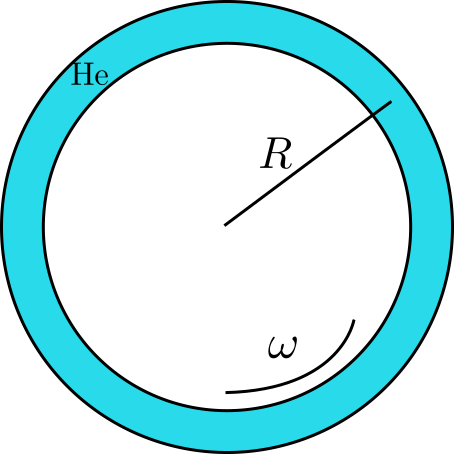
\includegraphics[width=.5\linewidth]{torus}
  \caption{
    % 
    The multiply connected toroidal geometry, of radius $R$, used to
    showcase superfluid behaviour. The anullus, which contains ${}^4$He
    atoms, rotates at an angular velocity $\omega$.
    % 
  }\label{fig:torus}
\end{figure}
% 
Assuming the pipe of radius $R$ is filled with liquid helium, and
rotates with angular velocity $\omega$, one can then obtain the
(temperature-dependent) orbital angular momentum of the system $L(T)$
by minimizing the effective free energy~\cite{leggett2006quantum}
%
\begin{equation}\label{eq:HF-angularmom}
  L(T) = I\left[f_n(T)\omega + f_s(T)n_w\omega_0\right]
\end{equation}
% 
Apart from the already defined quantities, we have introduced the
moment of inertia $I = N_0mR^2$, and defined the quantum unit of
angular velocity, $\omega_0 \equiv \hbar/(mR^2)$. Finally, $n_w$ is the
nearest integer to $\omega/\omega_0$, expressed as
%
\begin{equation}\label{eq:nearest-integer}
  n_w = \text{int} \left[\frac{\omega}{\omega_0} + \frac{1}{2}\right]
\end{equation}
% 
One needs to compare Eq.~\eqref{eq:HF-angularmom} with the angular
momentum of a normal liquid under the same circumstances, which is
given by $L = I \omega = N_0 \hbar \omega/\omega_0$. Keeping this in
mind, we can now introduce the two qualitatively different
experiments.


\paragraph{Persistent currents}
%
% protocol
%
The first experiment starts by rotating the torus at a large angular
velocity $\Omega \gg \omega_0$, on the high-temperature side of the
$\lambda$-point. Once the fluid equilibrates with the motion of the
container walls, we then cool the system through $T_{\lambda}$,
maintaining the same angular velocity $\Omega$. Finally, we stop the
container from rotating, and measure the angular momentum.
%
% observation
%
After a short while, proportional to the viscosity of the normal
component, its velocity $\bm{v}_n$ becomes zero. However, the
superfluid part of the liquid experiences no friction with the pipe
walls, and will therefore continue circulating indefinately! Since we
are not dealing with the ground state of the system, but with an
excited state with astronomical lifetime, we call this phenomenon
\textit{metastability of supercurrents} (``persistent currents'' is
another commonly found term).
%
% explanation
%
However, metastability of superflow is not a direct consequence of the
BEC state -- the underlying mechanism is one of topological origin:
consider the contour $C$ in Eq.~\eqref{eq:feynman} to run around the
torus of Fig.~\ref{fig:torus}. The current in the ring will be
proportional to the circulation Eq.~\eqref{eq:feynman}. Since the
latter is quantized, the windinding number $n_w$ is conserved, hence
so is the (super)current!
%
% vortices
%
Similar arguments explain the existence of so-called topological
defects in superfluid systems. Such defects are singularities of the
condensate wavefunction, for instance, vortex lines (or rings, if the
line closes in on itself) associated with the superfluid
component. The conservation laws presented above make the vortex a
highly stable configuration, as opposed to the case of a normal fluid,
where it is short-lived. In this sense, the circulating currents which
constitute the vortex are "persistent", corresponding to metastable
supercurrents. Furthermoe, a superfluid system cannot sustain bulk
vorticity due to Eq.~\eqref{eq:vorticity}, and the vortices are
quantized according to Eq.~\eqref{eq:feynman}.

In the final state with the container at rest, $\omega = 0$, so the
first term of Eq.~\eqref{eq:HF-angularmom} dissapears. The second term
survives, as the system cannot change its winding number. In the limit
of large $n_w$ the angular momentum will then be approximately given
by $L(T) \simeq f_s(T) I \Omega$. We see that one can reversibly
increase (or decrease) the angular momentum $L$ by varying the
temperature (provided, of course, that it is always kept below
$T_{\lambda}$).
%
% Landau criterion
%
Since the superfluid circulates despite any roughness of the container
walls, we can reasonably expect that an object moving though a
stationary fluid also experiences reduced friction. This led to a
series of experiments with charged ions being accelerated at various
speeds by an applied external electric field~\cite{Meyer1961,
  Allum1977}. It was seen that, in accordance with the Landau
criterion presented in Sec.~\ref{sec:cherenkov-emission}, there exists
a critical speed below which the ions experience reduced viscosity
(and actually no viscosity at all in the $T=0$ limit).



\paragraph{HF effect}
We now turn to the second experiment, which is arguably one of the
fundamental defining properties of superfluidity. The effect was first
predicted by Fritz London and then observed by G. Hess and W. Fairbank
in 1967 in the context of liquid helium, hence the name Hess-Fairbank
(HF) effect.
%
% protocol
%
As before, we cool the sample while rotating with a lower angular
velocity $\omega \ll \Omega$. We wait for the system to equilibrate,
and then measure the angular momentum, this time without stopping the
rotation of the container.
%
% observation
%
The value of $L$ will be given by Eq.~\eqref{eq:HF-angularmom},
instead of the classical $I \omega$ (that is why the HF effect is also
called nonclassical rotational inertia, NCRI).
%
We can now distinguish two different regimes. The first one, for
$\omega < \frac{1}{2}\omega_0$, implies $n_w = 0$, therefore
$L(T) = f_n(T)I\omega$, so the superfluid component contributes
nothing to the current. At $T=0$, $f_n(T) \rightarrow 0$ and we get
the spectacular result that the liquid completely ceases to rotate
along with the container!
%
In the general case, the second term of Eq.~\eqref{eq:HF-angularmom}
survives. If we again consider the zero-temperature limit, and plot
the angular momentum $L(0) = I\omega_0 n_w$ versus angular velocity
$\omega \geq \frac{1}{2}\omega_0$, we get a series of plateaus of
width $\omega_0$ at positions
$L = N_0 \hbar n_w = N_0 \hbar,\, 2N_0 \hbar$, and so on. The centers
of these plateaus all fall on the ``classical'' line
$L = N_0\hbar \omega/\omega_0$.
%
% explanation
%
A hand-waving explanation, for the simplest case of a noninteracting
atomic gas, goes as follows. In a noncondensed system rotating with
angular velocity $\omega$, the effective single-particle energies are
shifted by an amount $\hbar\omega \ell_{n_w}$, with $\ell_{n_w}$ the
angular momentum quantum number of state $n_w$. The Bose-Einstein
function then redistributes the particles to accomodate this shift,
producing a ``classical'' angular momentum. In a BEC however, all
$N_0$ atoms must be in the same state $n_w$, and posess the same value
of $\ell_{n_w}$. Their only allowed contribution to $L$ is then
$N_0(n_w\hbar)$. For small $\omega$, the condensate is in the
$n_w = 0$ state, and so it does not rotate with the container! This
argument can be formalized, so one can show the HF effect to be
impossible inside the framework of classical statistical mechanics,
much like the Bohr-Van Leeuwen theorem shows magnetism to be a purely
quantum phenomenon. Note that, while the HF effect can be (at least
hand-wavingly) explained without including interactions, these are
crucial to any theory of metastable currents.


\paragraph{Meissner effect}
As already explained in the introductory paragraph of this Section,
there is a deep underlying connection between superfluidity in a
neutral system and superconductivity in a charged one. In fact, the
analog of the HF effect in a charged system is the well-known Meissner
effect.
%
We now consider the same topology of Fig.~\ref{fig:torus}, and replace
the container by a crystal lattice and the liquid helium (or atomic
gas for that matter) by the electrons inside this lattice. If we now
keep the crystal at rest and produce a tangential vector potential
$\bm{A}(\rv) = A\hat{\phi}$, this will generate a flux
$\Phi = \oint \bm{A}(\rv)\cdot d\bm{l}$ inside the conducting ring
(usually called an ``Aharonov-Bohm''
flux). The definition of the ``superfluid''
velocity Eq.~\eqref{eq:supervelocity} now needs to be revised
according to the gauge-coupling recipe, which consists of replacing
the canonical momentum $\bm{p}$ by the kinematic one:
$\bm{p} \rightarrow \bm{p} - e\bm{A}(\rv)$. As a result, we get
%
\begin{equation}\label{eq:superconducting-velocity}
  \bm{v}_s(\rv) = \frac{1}{2m}\left(\bm{\nabla}\theta(\rv) -
    2e\bm{A}(\rv)\right)
\end{equation}
% 
where the factors of 2 appear because the macroscopic wavefunction is
now that of the center of mass of a Cooper-pair of electrons, so $m$
and $e$ are both multiplied by 2. The resulting Onsager-Feynman
quantization Eq.~\eqref{eq:feynman} then becomes
%
\begin{equation}\label{eq:superconducting-feynman}
  \oint_C \bm{v}_s(\rv) \cdot d\bm{l} = \frac{\hbar}{2m} \left(2\pi n_w -
    \frac{\Phi}{\Phi_0}\right)
\end{equation}
% 
where $\Phi_0 \equiv h/(2e)$ is the \textit{superconducting flux
  quantum}. If the (mass) supercurrent is given, as before, by
$\bm{j}_s = \rho_s \bm{v}_s$, then this new quantization condition
results in a non-zero current even for $n_w = 0$. Indeed, for
$\Phi < \frac{1}{2} \Phi_0$ (compare to the regime
$\omega < \frac{1}{2}\omega_0$ discussed for the HF effect), the
$n_w = 0$ state is realized and the electrical current $\bm{j}_e$ is
given by
%
\begin{equation}\label{eq:diamagnet}
  \bm{j}_e(\rv) = \frac{2e}{2m}\bm{j}_s = - \frac{e^2}{m^2}\rho_s(T) \bm{A}(\rv)
\end{equation}
%
This proves that, while in a normal conductor the flux $\Phi$ would
not generate any circulating current, a superconducting ring would
respond with a diamagnetic (note the minus sign in
Eq.~\eqref{eq:diamagnet}) electrical current proportional\footnote{The
  proportionality constant is called the susceptibility.} to the
vector potential $\bm{A}$. Coupling this with Maxwell's equations
immediately results in the well-known Meissner effect, namely the
expulsion of an applied magnetic field inside a superconducting
sample.


\paragraph{Synthetic gauge field}
We now proceed to a closer analysis of the connection between the
charged and neutral case. The Hamiltonian $H$ for a particle of charge
$q$ and mass $m$, moving in a vector potential $\bm{A}$, and in the
presence of an external potential $V$, is given by
Eq.~\eqref{eq:charged-ham}. In our problem, $V$ is imposed by the
toroidal geometry of the container, which is for now assumed to be
stationary in the inertial frame of the stars. On the other hand, the
Hamiltonian $H^{\prime}$, of a neutral particle with the same mass,
but this time in the frame that rotates with the container at an
angular velocity $\bm{\omega} = \omega\hat{z}$ is shown in
Eq.~\eqref{eq:neutral-ham},
%
\begin{align}
    H  = \frac{1}{2m}(\bm{p} - q\bm{A}(\rv))^2 & + V(\rv)\label{eq:charged-ham}\\
    H^{\prime}  = \frac{1}{2m}(\bm{p}^{\prime}-m\bm{\omega}\times
    \rv^{\prime})^2 & + V(\rv^{\prime}) - \frac{1}{2}m(\bm{\omega}\times
    \rv^{\prime})^2\label{eq:neutral-ham}
\end{align}
%
with $\rv^{\prime}$ being the coordinate (and $\bm{p}^{\prime}$ the
canonical momentum) in the rotating frame. Making use of the
cylindrical symmetry, one can decompose $\rv$ as $(r,\,z,\,\theta)$,
and therefore $\rv^{\prime} = (r,\,z,\,\theta-\omega t)$.
%
We now see that a neutral system in the rotating frame, apart from a
centrifugal term $- \frac{1}{2}m(\bm{\omega}\times \rv^{\prime})^2$,
is formally identical to a charged system in the rest frame, with the
correspondence $q\bm{A}(\rv) \leftrightarrow m\bm{\omega}\times
\rv$. This connection can be used to make a neutral particle
experience an ``effective'' electromagnetic vector potential. Its
gauge-coupling to this potential is what eventually led to the
celebrated concept of \textit{synthetic gauge field}.
%
In fact, such artificial, rotation-induced, gauge fields have already
been proposed in the context of ultracold atomic gases, in order to
asess their normal and superfluid
fractions~\cite{Cooper2010,Carusotto2011,John2011}.


\paragraph{BEC Experiments}
%
\begin{figure}[tb]\centering
  \includegraphics[width=.8\linewidth]{hole}
  \caption{
    % 
    Scanning a blue-detuned laser beam with velocity $v$, though the
    cigar-shaped atomic condensate (left panel), creates a density hole
    (right panel) larger than the healing length. The friction acting on
    this hole can then be used to asess the Landau critical velocity. From
    Ref.~\cite{Raman_1999}.
    % 
  }\label{fig:hole}
\end{figure}
% 
This naturally leads us to the topic of experimental evidence for
superfluid behaviour. The answer, however, will not be a clear-cut
one, as we have seen that it actually depends on which aspects of
superfluidity one is interested in, such as NCRI, persistent currents,
quantized vortices or reduced friction on impurities. Historically,
liquid ${}^4$He-II was the default system for exploring such physics,
however, new systems such as ultracold gases and, more recently,
microcavity polaritons (the subject of Chapter~\ref{cha:polaritons})
have also entered the picture. In the case of liquid helium,
superfluidity is relatively easy to detect, while BEC can only be
asessed through circumstantial evidence (such as neutron scattering),
as strong interactions oppose any large density changes. Ultracold
gases, on the other hand, present a spectacular BEC onset that can be
observed in the density profile, while superfluidity proves somewhat
more mysterious.
%
Regarding metastable supercurrents in a simply connected geometry,
Chevy and coworkers~\cite{Chevy2000} succeded in stirring an atomic
condensate, and then measuring its angular momentum using the
precession of certain collective modes.  Other studies were also shown
to produce a metastable single-vortex state (and even vortex lattices)
that persist, despite not being the ground state of the system (in
fact, it can be shown that the atomic BEC ground state is
characterised by the absence of any macroscopic current flow).
Interferometric measurements are commonly employed to see the
circulation around these vortex cores.  However, the lifetime of the
vortices is limited by how long it takes before they escape the
magnetic trap. To circumvent this limitation, persistent currents in
multiply connected geometries (such as toroidal traps) were also
investigated, for instance in Refs.~\cite{Ryu2007}
and~\cite{Ramanathan2011}.
% 
As far as the Landau criterion is concerned, an experiment similar to
the one accelerating charged ions through liquid helium was reported
in Ref.~\cite{Chikkatur_2000}. The authors used a Raman laser to
transfer a fraction of the condensed atoms into a different
(hyperfine) state. As a result, those atoms no longer experienced any
magnetic trapping, but only the effect of gravity. The mobility of the
free-falling atoms was then computed, revealing information about the
friction~\cite{Astrakharchik_2004} acting on them.  A fairly sharp
transition with a sudden increase in friction was observed, at
velocities close to the local speed of sound.
%
In the opposite limit of macroscopic ``impurities'' (large compared to
the healing length), Ref.~\cite{Onofrio_2000} details the use of a
blue-detuned laser beam, in order to create a density hole which is
then moved around the atomic condensate (see Fig.~\ref{fig:hole}).  By
measuring the density difference immediately ahead and behind the
hole, one can deduce the frictional force acting on it (see
Appendix~\ref{app:field-theory}). This experiment resulted in a
critical velocity about ten times smaller than the speed of sound,
presumably due to vortex creation by the macroscopic defect.


\section{Optical lattices}
\label{sec:optical-lattice}

\paragraph{Laser trapping}
An electric dipole moment $\bm{\mathcal{P}}$ placed in an external
electric field $\bm{\mathcal{E}}(\rv)$ aquires an energy
$\mathcal{V}(\rv) = -\bm{\mathcal{P}}\cdot \bm{\mathcal{E}}(\rv)$. If
an atom is placed in a light field, the oscillating electric field of
the latter induces an electric dipole moment
$\bm{\mathcal{P}} = \alpha \epsilon_0 \bm{\mathcal{E}}$ on the atom,
with $\epsilon_0$ the free-space permittivity and $\alpha$ the atomic
polarizability~\cite{feynman1979lectures}. Integrating, we obtain the
interaction energy of the atom with the field as
$\mathcal{V}(\rv) = -\frac{1}{2}\alpha \epsilon_0
\mathcal{E}^2(\rv)$. A classical model of the atom as a conducting
sphere of radius $r$ yields a polarizability of $4\pi r^3$. In
practice however, atomic transitions complicate this simple picture,
as the polarizability $\alpha$ depends on the driving frequency of the
light field. In the framework of the Drude
model~\cite{ziman1972principles}, one has
%
\begin{equation}\label{eq:polarizability}
  \alpha(\omega) = \frac{\alpha(0)\omega_0^2}{\omega_0^2 - \omega^2 - i \frac{\omega}{\tau}}
\end{equation}
% 
with the resonant frequency $\omega_0$, damping time $\tau$ and
$\alpha(0) > 0$ the static polarizability. The frequency-dependent
interaction energy $\mathcal{V}(\omega)$ thus obtained is sometimes
called the \textit{ac Stark effect}~\cite{Cohen-Tannoudji:101392}. If
the light frequency is smaller than that of the atomic resonance
$\omega < \omega_0$, the induced dipole is in phase with the electric
field, as $\Re[\alpha(\omega)] > 0$, and the force on the atom will
point in the direction of the square-field maxima (the situation is of
course reversed if instead $\omega > \omega_0$). This effect was first
used in Ref.~\cite{PhysRevLett.80.2027} to trap a BEC of sodium atoms
using a focused infrared laser beam (the dominant transition of Na is
the familiar $s \rightarrow p$ yellow emission). Interestingly, the
same physics can be used to create an optical lattice, as explained
below.

\paragraph{Optical lattice}
Consider a (plane wave) laser beam propagating along the $x$ axis,
with an associated electric field
$\bm{\mathcal{E}}(x,t) = \bm{\mathcal{E}}_0 \cos (k_x x - \omega t)$,
which reflects from a mirror situated at $x=0$. The interference
between the reflected and original beam produces a standing wave
$\bm{\mathcal{E}}_0[\cos(k_x x - \omega t) - \cos(k_x x + \omega t)]$,
with an intensity
$\abs{\mathcal{E}(x,t)}^2 = 4 \abs{\mathcal{E}_0}^2 \sin^2(k_x
x)\sin^2(\omega t)$. This results in an effective periodic lattice for
the atoms, with lattice spacing $b = \lambda_x/2$, where
$\lambda_x = 2\pi/k_x$. Such a one-dimensional lattice was first
demonstrated in Ref.~\cite{Anderson1686}. By tuning the strength of
the laser field, one can adjust the lattice depth, and by changing the
laser wavelength, one can modify the lattice constant. Adding more
laser beams can produce two- or even three-dimensional lattices, in a
variety of different geometries. For example, the simplest way to
create a 2D square lattice would be to superimpose a second lattice in
the $\hat{\bm{y}}$ direction, producing an optical potential of depth
$V_0$:
%
\begin{equation}\label{eq:square-potential}
  \mathcal{V}(x,y) = V_0[\sin^2(\pi x/b) + \sin^2(\pi y/b)]
\end{equation}
% 
The beam along $y$ should be orthogonally polarized with respect to
the one along $x$, in order to avoid interference effects.

\paragraph{Band structure}
The eigen-problem of a particle moving in a periodic potential given
by Eq.~\eqref{eq:square-potential} is well-known in the context of
solid-state band theory~\cite{ziman1972principles}, as the electrons
inside a solid also move in such a potential, produced in that case by
the crystal ions. The energy eigenstates are the Bloch waves
$\psi_{\gamma,\kv}(\rv) = e^{i\kv\cdot\rv} u_{\gamma,\kv}(\rv)$, where
$\hbar \kv$ is the \textit{quasimomentum}, restricted to the first
Brillouin zone (BZ)
$\left(-\frac{\pi}{b}, \frac{\pi}{b}\right) \times
\left(-\frac{\pi}{b}, \frac{\pi}{b}\right)$ and $\gamma = 0,1,\dots$
represents the \textit{band index}. The functions
$u_{\gamma,\kv}(\rv)$ are periodic in both the $\hat{\bm{x}}$ and
$\hat{\bm{y}}$ direction, with period $b$. To see how these bands
arise, one can expand both the wavefunction $\psi_{\gamma,\kv}$ as
well as the potential $\mathcal{V}$ in a Fourier series, making use of
their periodicity. Inserting this expansion into the time-independent
Schr\"odinger equation, we get a linear system of equations for the
Fourier coefficients. For fixed $\kv$, we obtain
different\footnote{Truncating the Fourier expansion to a finite number
  of terms $n$ results in $2n+1$ bands.} eigenenergies,
$E_{\gamma}(\kv)$. These eigenenergies form bands (called \text{Bloch
  bands}) when $\kv$ is varied inside the BZ. Each band as a certain
width in energy (unsurprisingly called the bandwidth) and consecutive
bands are separated by gaps, meaning certain energies are not
allowed. Furthermore, each eigenenergy has an associated
eigenfunction, completely determined by the set of Fourier
coefficients with index $\gamma$. The solution of course depends on
the value of $V_0$, and we can distinguish two limiting cases,
depending on the ratio of the bandwidths to the energy gaps. In the
weak-potential limit, the bandgaps are much smaller than the
bandwidths, and the eigenenergies have a pronounced dependence on
quasimomentum. The opposite limit, which is the one we want to focus
on, is the regime of deep lattices, also called the
\textit{tight-binding} (TB) limit. The band dispersion is now flatter
compared to the previous case, and the bandwidth/gap ratio is much
smaller.

\paragraph{Tight binding}
For low temperatures in the TB limit, only the lowest energy band
$\gamma = 0$ is occupied, so we subsequently drop the band
index. Since the potential wells are so deep, the lowest band is
adequately described by considering localized wavefunctions at each
well, i.e. at the minima of Eq.~\eqref{eq:square-potential}. Suppose
now that a function $w(\rv)$ exists such that the Bloch waves are
given by
%
\begin{equation}\label{eq:wanier}
  \psi_{\kv} (\rv) = \mathcal{N} \sum_{m,n} e^{i\kv \cdot \rv_{m,n}} w(\rv - \rv_{m,n})
\end{equation}
% 
where $\mathcal{N}$ is a normalization factor and
$\bm{r}_{m,n} = m b \hat{\bm{x}} + n b \hat{\bm{y}}$ are the well
positions. Eq.~\eqref{eq:wanier} represents a wave,
$e^{i\kv \cdot \rv_{m,n}}$, whose phase and amplitude at each well is
given by the localized function $w$, called the \textit{Wannier
  function}~\cite{ziman1972principles}. It can be shown that Wannier
functions centered at different wells are orthogonal to each other and
form a complete basis. The Wannier functions are thus a unitary
transformation of the Bloch functions, suitable for the case when
particle dynamics is described by inter-well tunneling (hopping)
between nearest-neighbour wells. 

In the case of a BEC, when the number of ultracold atoms per lattice
well is small, the ``discrete structure'' of the condensate becomes
relevant and we must replace the GP description Eq.~\eqref{eq:TDGP} we
have used so far with a lattice model, such as the Bose-Hubbard
model~\cite{PhysRevB.40.546}, as suggested in
Ref.~\cite{Jaksch3108}. For a condensate confined in the optical
potential Eq.~\eqref{eq:square-potential}, with an additional harmonic
trap $U(\rv)$, the spinless Bose-Hubbard Hamiltonian in 2D can be
written as~\cite{zwerger2003}
%
\begin{equation}\label{eq:BH-ham}
  \mathcal{H}\sub{BH} = \mathcal{H}_0 + \frac{U}{2}\sum_{m,n} \hat{n}_{m,n}(\hat{n}_{m,n} - 1) + \sum_{m,n} \epsilon_{m,n} \hat{n}_{m,n}
\end{equation}
% 
where $U \propto g$ is the on-site interaction strength and
$\epsilon_{m,n} \propto U(\rv_{m,n})$ is the energy offset due to the
harmonic trap. Futhermore,
$\hat{n}_{m,n} = \hat{a}_{m,n}^{\dagger} \hat{a}_{m,n}$ denotes the
number operator for site $(m,n)$ and $\hat{a}_{m,n}^{\dagger}$
($\hat{a}_{m,n}$) is the bosonic creation (destruction) operator for
that site. Finally, the kinetic part
%
\begin{equation}\label{eq:kinetic-part}
  \mathcal{H}_0 = -J \sum_{m,n} \left(\hat{a}^{\dagger}_{m+1,n}\hat{a}_{m,n} + \hat{a}^{\dagger}_{m,n+1}\hat{a}_{m,n}\right) + \text{H.c.}
\end{equation}
% 
can be diagonalized to yield the Bloch dispersion
%
\begin{equation}\label{eq:tb-dispersion}
  E(\kv) = -2J\left[\cos(k_x b) + \cos(k_y b)\right]
\end{equation}
% 
where the tunneling amplitude $J$ is an exponentially decreasing
function of $V_0$~\cite{zwerger2003}. The characteristic tunneling
energy scale is given by the bandwidth, which in this case is $8J$.

Hamiltonian Eq.~\eqref{eq:BH-ham} supports a zero-temperature quantum
phase transition between a superfluid and a Mott-insulating phase, at
a critical value of the ratio $U/J$. This transition was
experimentally observed for the case of a bosonic BEC in a 3D optical
lattice, as reported in Ref.~\cite{greiner2002quantum}. Increasing the
lattice depth $V_0$, the authors went from a gapless, superfluid
regime dominated by the kinetic term Eq.~\eqref{eq:kinetic-part} to a
gapped Mott-insulator state, where the atoms are localized and the
on-site interaction term in Eq.~\eqref{eq:BH-ham} is dominant.

\section{Harper-Hofstadter model}
\label{sec:hh-atoms}
\paragraph{Landau levels}
In Sec.~\ref{sec:optical-lattice} we introduced the quantized Bloch
bands, characterising particles in a periodic potential. A similar
quantization also occurs in the case of a charged particle moving
perpendicular to a constant uniform magnetic field, and the allowed
energy bands are called \textit{Landau
  levels}~\cite{Landau:101810}. In a magnetic field
$\bm{B} = B \hat{\bm{z}}$, the relevant energy and length scales for a
particle with charge $e$ and mass $m$ are set by the \textit{cyclotron
  frequency} $\omega_c = eB/m$ and \textit{magnetic length}
$l\sub{m} = \sqrt{\hbar/eB}$, respectively. In this Section we want to
explore the fate of the Bloch bands in presence of a magnetic
field. Alternatively, one could also start from a Landau quantized
system and perturb it via a weak periodic
potential~\cite{PhysRev.180.633,PhysRevB.46.12606}, the two approaches
having distinct validity ranges.

\paragraph{Hofstadter butterfly}
One of the simplest TB models for Bloch electrons in uniform magnetic
fields is the \textit{Harper-Hofstadter
  model}~\cite{harper1955magnetic,hofstadter1976butterfly}. Its
relevant dimensionless parameter is the ratio of flux $\Phi$ through a
lattice cell to one \textit{Dirac flux quantum}\footnote{As opposed to
  the superconducting flux quantum of Sec.~\ref{sec:superfluid-atom}.}
$\Phi_0=h/e$
%
\begin{equation}\label{eq:alpha}
  \alpha = \frac{\Phi}{\Phi_0} = \frac{eBb^2}{h}
\end{equation}
% 
Physically, $\alpha$ reflects\footnote{Not to be confused with the
  atomic polarizability, also denoted by $\alpha$.} the
commensurability of the lattice period $b$ and the magnetic length
$l\sub{m}$, as it can be recast in the form
$\alpha = \frac{1}{2\pi}\left(b/l\sub{m}\right)^2$.  The resulting
single-particle energy spectrum of the model depends on the
rationality of $\alpha$. If $\alpha = p/q$, for $p$ and $q$ co-prime
integers, the Bloch band splits into $q$ distinct magnetic
subbands. For $\alpha$ irrational, the spectrum consists instead of an
infinite number of energy levels, forming a Cantor set. The union of
all allowed energies as a function of $\alpha$ forms a self-similar
fractal, shown in Fig.~\ref{fig:butterfly} and known as
\textit{Hofstadter’s butterfly}~\cite{hofstadter1976butterfly}. In the
continuum limit ($b \rightarrow 0$, with fixed $B$), $\alpha \ll 1$
and the bands group into clusters that can be identified with the
Landau fan predicted in the absence of a lattice potential.
%
\begin{figure}[tb]\centering
  \includegraphics[width=\linewidth]{hhbutterfly}
  \caption{
    % 
    Hofstadter's butterfly, representing the internal structure of the
    lowest Bloch band in a uniform magnetic field. For rational values of $\alpha
    = p/q$, the spectrum has $q$ magnetic subbands, which become
    increasingly narrow as $q$ gets larger. Adapted from
    Ref.~\cite{hofstadter1976butterfly}.
    % 
  }\label{fig:butterfly}
\end{figure}
% 

\paragraph{HH experiments}
Solid-state experiments in the Hofstadter regime are notoriously
difficult, since the inter-atomic spacing of a crystal lattice is a
few {\AA}ngstr\"oms, and achieving a comparable magnetic length would
require a field of about $10^4$ Tesla. Signatures of the Hofstadter
bands have instead been seen in artificial superlattices with
periodicities of tens of
nanometers~\cite{dean2013hofstadter,yu2014hierarchy}. In the context
of neutral ultracold atoms, synthetic gauge potentials paved the way
for the exploration of similar
physics~\cite{dalibardrmp2011,goldman_repprog_2014}. For instance,
rotating a harmonically trapped condensate with a high angular
velocity (comparable to the radial trap frequency) allowed BEC
experiments~\cite{PhysRevLett.92.040404} to enter the lowest Landau
level (LLL) regime. Rotating 2D optical lattices have also been
realized~\cite{PhysRevLett.104.050404}, but the first implementation
of the Harper-Hofstadter (HH) model with ultracold
atoms~\cite{aidelsburger2013hh,miyake2013hh} employed a different
method~\cite{goldman_repprog_2014} of generating the artificial
magnetic field, namely \textit{laser-assisted
  tunneling}~\cite{1367-2630-5-1-356} based on a linear superlattice
potential~\cite{1367-2630-12-3-033007}. In a nutshell, tunneling
between lattice sites required atoms to absorb and emit photons
produced by external lasers. The interaction with said lasers
generated a net phase change equivalent to the flux of a magnetic
field. The total phase accumulated by an atom when performing a loop
around a lattice cell (plaquette) was $\sim \pi/2$ in these
experiments.

\paragraph{Aharonov-Bohm phase}
In quantum mechanics, the phase of the wavefunction of a charged
particle moving between positions $\rv_1$ and $\rv_2$ is changed by
the presence of a magnetic field $\bm{B} = \bm{\nabla} \times \bm{A}$
by~\cite{feynman1979lectures}
%
\begin{equation}\label{eq:AB-phase}
  \phi_{12} = \frac{e}{\hbar}\int_{{\rv}_{1}}^{{\rv}_{2}} d\rv \cdot \bm{A}(\rv)
\end{equation}
% 
where the integral is taken along an oriented path from point ``1'' to
point ``2''. Therefore, $\phi_{21} = -\phi_{12}$ and, if we consider a
smooth closed integration contour $\mathcal{C}$ instead of two
separate points, the total phase change (or \textit{Aharonov-Bohm
  phase}) along $\mathcal{C}$ is
%
\begin{equation}\label{eq:AB-closed}
  \phi_{\mathcal{C}} = \frac{e}{\hbar}\int_{\mathcal{S}}
  d^2 \rv \cdot \bm{\nabla} \times
  \bm{A}(\rv) = 2\pi \frac{\Phi_B}{\Phi_0}
\end{equation}
% 
where $\Phi_B$ is the magnetic flux through a smooth surface
$\mathcal{S}$ bounded by the curve $\mathcal{C}$ with positive
orientation, according to Stoke's theorem.

\paragraph{Peierls phases}
On the 2D square lattice in Fig.~\ref{fig:hh-lattice}, one can define
the magnetic phases
$\phi_{m,n} = \left(\phi^{x}_{m,n},\phi^{y}_{m,n}\right)$ along the
$\hat{\bm{x}}$ and $\hat{\bm{y}}$ directions in a similar manner, as
%
\begin{figure}[tb]\centering
  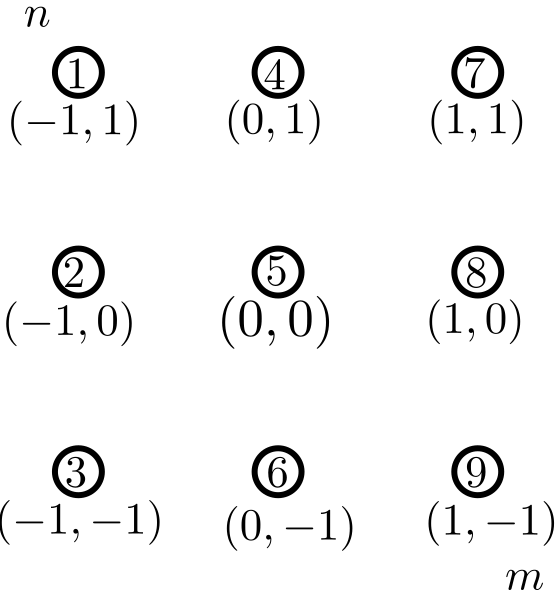
\includegraphics[width=.4\linewidth]{lattice}
  \caption{
    % 
    2D square lattice pierced by a homogeneous static magnetic field
    $\bm{B} = B\hat{\bm{z}}$. The lattice constant is $b$, and the curved
    arrows indicate the field-induced hopping phases.
    % 
  }\label{fig:hh-lattice}
\end{figure}
%
\begin{align}
  \phi^{x}_{m,n} &= \frac{e}{\hbar}\int_{{\rv}_{m,n}}^{{\rv}_{m+1,n}} d\rv \cdot \bm{A}(\rv) &
  \phi^{y}_{m,n} &= \frac{e}{\hbar}\int_{{\rv}_{m,n}}^{{\rv}_{m,n+1}} d\rv \cdot \bm{A}(\rv)
\end{align}
where the integrals are now taken along the links joining neighbouring
sites. Using Eq.~\eqref{eq:AB-closed}, the flux $\Phi$ through a
plaquette can be related to the total phase $\phi_{\square}$
accumulated on a contour enclosing the plaquette in a counterclockwise
sense
%
\begin{equation}\label{eq:lattice-curl}
  \phi_{\square} \equiv \sum_{\circlearrowleft
    \square} \phi_{m,n} =  \phi^x_{m,n} + \phi^y_{m+1,n} - \phi^x_{m,n+1} - \phi^y_{m,n} = 2\pi \alpha 
\end{equation}
% 
Note that $\phi_{\square}$ is gauge-independent, unlike the
\textit{Peierls phases} $\phi_{m,n}$.



\paragraph{HH Hamiltonian}
To obtain the HH Hamiltonian, we introduce a static uniform magnetic
field into the single-band Bose-Hubbard model Eq.~\eqref{eq:BH-ham} of
Sec.~\ref{sec:optical-lattice}. We follow Hofstadter's original
treatment, and neglect on-site interactions\footnote{For a treatment
  that includes interactions in the Bogoliubov approximation, see
  Ref.~\cite{PhysRevA.83.013612}.}, as well as the harmonic
trapping. The kinetic term Eq.~\eqref{eq:kinetic-part} is then
modified according to Peierls' substitution~\cite{peierls1933} to
include the hopping phases $\phi_{m,n}$
%
\begin{equation}\label{eq:HH-hamiltonian}
  \mathcal{H}_0 = -J \sum_{m,n} \left(e^{i\phi^x_{m,n}}\hat{a}^{\dagger}_{m+1,n}\hat{a}_{m,n} + e^{i\phi^{y}_{m,n}}\hat{a}^{\dagger}_{m,n+1}\hat{a}_{m,n}\right) + \text{H.c.}
\end{equation}
% 
These phases act to ``frustrate'' the hopping, such that for
noninteger $\alpha$ it is impossible to minimize the kinetic energy
simultaneously on all lattice links~\cite{moessner2001}. The
Hamiltonian is no longer invariant under translations by a single
lattice site in any direction, because fixing a gauge for the vector
potential $\bm{A}(\rv)$ reduces the physical symmetry of the
lattice. In fact, it can be shown~\cite{jain2007composite} that a
translation of $\bm{A}$ is equivalent to a gauge transformation,
suggesting that new translation operators that would commute with
Eq.~\eqref{eq:HH-hamiltonian} can be constructed as a combination of
translation and gauge transformation.


\paragraph{Magnetic translation operators}
We define the \textit{magnetic translation operators} (MTOs)
~\cite{zak1964group,zak1964representations} as

%
\begin{align}
  \tx &= \sum_{m,n} \hat{a}^{\dagger}_{m+1,n}\hat{a}_{m,n}e^{i\theta^x_{m,n}} &
  \ty &= \sum_{m,n} \hat{a}^{\dagger}_{m,n+1}\hat{a}_{m,n}e^{i\theta^y_{m,n}}
\end{align}
%
where the phases $\theta_{m,n}$ are to be determined by imposing
$\left[\hat{T}, \mathcal{H}_0 \right] = 0$, leading
to~\cite{bernevig2013topological}
%
\begin{align}
  \theta^x_{m,n} &= \phi^x_{m,n} + 2\pi\alpha n &
  \theta^y_{m,n} &= \phi^y_{m,n} - 2\pi\alpha m 
\end{align}
% 
While the specific form of the MTOs depends on the choice of gauge,
their commutator is gauge independent
%
\begin{equation}\label{eq:TxTy}
  \tx \ty = \ty \tx  e^{i2\pi\alpha} 
\end{equation}
% 
and vanishes only if $\alpha$ is an integer, a situation equivalent to
the zero-field case. In order to proceed, we point out that
Eq.~\eqref{eq:TxTy} has a transparent physical interpretation. If we
act on the single-particle state
$\ket{m,n} = \hat{a}^{\dagger}_{m,n}\ket{0}$
%
\begin{equation}\label{eq:translation-loop}
  \ty^{\dagger} \tx^{\dagger} \ty \tx \ket{m,n} = e^{-i2\pi\alpha} \ket{m,n}
\end{equation}
%
we see that performing a counterclockwise loop around a unit cell
results in the accumulation of a phase proportional to the flux inside
the cell. This can be generalized to a macrocell containing
$r \times s$ original lattice cells, to deduce that
%
\begin{equation}
  \tx^r\ty^s = \ty^s\tx^re^{i(rs)2\pi\alpha}
\end{equation}
% 
For $\alpha = p/q$ the commutator $\left[\tx^r, \ty^s\right]$ vanishes
if $p (rs)/q$ is an integer. The smallest possible macrocell is given
by $rs = q$ and is called the \textit{magnetic unit cell}. For this
choice of unit cell, $\{\tx^r, \ty^s, \mathcal{H}_0\}$ form a complete
set of commuting operators, so we can find simultaneous eigenstates,
labeled by the quasimomentum $\hbar\kv^0$ which is now restricted to
the \textit{magnetic Brillouin zone} (MBZ)
$\left(-\frac{\pi}{rb}, \frac{\pi}{rb}\right) \times
\left(-\frac{\pi}{sb}, \frac{\pi}{sb}\right)$.


\paragraph{HH spectrum}
%
\begin{figure}[tb]\centering
  \includegraphics[width=\linewidth]{hhgapwidth}
  \caption{
    % 
    \emph{Top panels:} Single-particle energy spectrum (left)
    $E_n(k_x^0=0,k_y)$ of the HH Hamiltonian Eq.~\eqref{eq:HH-hamiltonian}
    for $\alpha = 1/7$ and dispersion of the two lowest bands, $E_0(\kv)$
    (middle) and $E_1(\kv)$ (right) in (part of) the MBZ.  \emph{Bottom
      panel:} Energy gap (continuous line) $\Delta E =
    \left<E_1(\vt{k})\right>_{\vt{k}} - \left<E_0(\vt{k})\right>_{\vt{k}}$
    (here $\left<\cdot\right>_{\vt{k}}$ denotes an average over the MBZ)
    and bandwidth of $E_0(\kv)$ (dashed line, $\times 10$) for $p =
    1$. The dotted vertical line marks the location of the $q = 7$ case
    shown above.
    % 
  }\label{fig:hh-energy-levels}
\end{figure}
% 
To obtain the spectrum of $\mathcal{H}_0$, we need to solve its
associated Schr\"odinger equation,
$\mathcal{H}_0\ket{\psi} = E\ket{\psi}$. We expand the eigenstates
$\ket{\psi}$ in the single-particle basis
$\ket{\psi} = \sum_{m,n} \psi_{m,n} \ket{m,n}$ and obtain an equation
for the coefficients $\psi_{m,n}$
%
\begin{multline}\label{eq:HH-schrodinger}
  -J \big(e^{-i\phi^x_{m,n}}\psi_{m+1,n}+e^{i\phi^x_{m-1,n}}\psi_{m-1,n}\\
  {} + e^{-i\phi^y_{m,n}}\psi_{m,n+1} + e^{i\phi^y_{m,n-1}}\psi_{m,n-1}\big) = E\psi_{m,n}
\end{multline}
% 
We fix the Landau gauge $\bm{A}(x,y)=Bx\hat{\bm{y}}$ for simplicity,
so $\phi_{m,n} = (0,2\pi\alpha m)$ and we choose the magnetic unit
cell\footnote{In the symmetric gauge, the magnetic unit cell is
  larger, containing $2q \times 2q$ sites.}
$r \times s = q \times 1$, for which the commuting MTOs read
%
\begin{align}
  \hat{T}^q_x &= \sum_{m,n} \hat{a}^{\dagger}_{m+q,n} \hat{a}_{m,n} &
  \hat{T}_y &= \sum_{m,n} \hat{a}^{\dagger}_{m,n+1} \hat{a}_{m,n}
\end{align}
%
justifying the plane wave ansatz\footnote{Here $k_y$ is defined in the
  full BZ.}  $\psi_{m,n} = e^{ik_ynb}e^{ik_x^0mb} \psi_m$ subject to
the periodic boundary conditions $\psi_{m+q} = \psi_m$. Substituting
this ansatz into Eq.~\eqref{eq:HH-schrodinger} yields the
\textit{Harper equation}~\cite{Harper_1955}
%
\begin{equation}\label{eq:Harper}
  -J\left[e^{-ik_x^0 b} \psi_{m-1} + 2\cos\left(k_yb - 2\pi\alpha m\right)\psi_m + e^{ik_x^0 b}\psi_{m+1}\right] = E\psi_m
\end{equation}
% 
Calculating the single-particle spectrum of
Eq.~\eqref{eq:HH-hamiltonian} is therefore equivalent to solving the
eigenvalue equation
$\sum_{m^{\prime}=0}^{q-1} H_{mm^{\prime}}\psi_{m^{\prime}} =
E\psi_m$, $m=0,\dots,q-1$ for the $q \times q$ matrix $H$ defined
as\footnote{If $q = 2$, $m+1 \bmod q = m-1 \bmod q$ and
  $H_{01} = H_{10} = -2J\cos (k_x^0b)$.}
%
\begin{equation}\label{eq:Hmatrix}
  H_{mm^{\prime}}(k_x^0,k_y) = -J\times\begin{cases}
    e^{-ik_x^0 b} & \text{if $m^{\prime} = m-1 \bmod q$}\\
    2\cos\left(k_yb - 2\pi\alpha m\right) & \text{if $m^{\prime} = m$}\\
    e^{ik_x^0 b}  & \text{if $m^{\prime} = m+1 \bmod q$}\\
    0 & \text{otherwise}
  \end{cases}
\end{equation}
%
For integer $\alpha$ we recover the lowest Bloch band
Eq.~\eqref{eq:tb-dispersion}, while for $\alpha = p/q$ this band
splits into $q$ bands with dispersion $E_n(k_x^0,k_y)$, $n =
0,\dots,q-1$. 

\paragraph{Spectrum discussion}
In the top-left panel of Fig.~\ref{fig:hh-energy-levels} we show an
example of the spectrum computed by diagonalizing $H$ for
$\alpha = 1/7$. The $E=0$ level is at the centre of the middle band,
and there are $q-1$ gaps separating the bands. For even values of $q$,
the spectrum is symmetric with respect to $E=0$ and the two central
bands touch at zero energy. Around these degeneracy points, the
dispersion is linear~\cite{PhysRevB.39.11943}, while in all other
cases it is quadratic near its minimum. The $\alpha=1/2$ case is
particularly interesting by analogy to graphene-related
physics~\cite{RevModPhys.81.109}, as there are two inequivalent
``Dirac points'' and the Hamiltonian preserves time-reversal
symmetry. Inspecting the middle and right panels we note that, despite
the reduced symmetry of $\mathcal{H}_0$, the dispersion has the full
$C_4$ rotational symmetry of the underlying square lattice. One can
formally define rotation and reflection operators which, together with
the MTOs, constitute the full \textit{projective symmetry
  group}~\cite{PhysRevB.65.165113}.  The bottom panel of
Fig.~\ref{fig:hh-energy-levels} shows the evolution of the lowest
energy gap $\Delta E$, as well as the bandwidth $BW$ of the lowest
band as function of $q$ (for the case $\alpha = 1/q$). The lowest band
gets flatter, as the continuum ($q \rightarrow \infty$) LLL
eigenstates are the solutions of the lowest band of the HH
model~\cite{bernevig2013topological}, and $\Delta E$ decreases like
$\sim 1/q$, as the number of gaps is $\sim q-1$ (excluding the band
bottom and band top).


\paragraph{HH topology}
The energy bands of the HH model are topologically nontrivial, as
characterized by their non-zero \textit{Chern numbers} -- topological
invariants that are linked to the quantization of the Hall
conductivity in the integer quantum Hall (QH)
effect~\cite{thouless}. In fact, solutions of the Harper equation
Eq.~\eqref{eq:Harper} were also studied in connection with the QH
effect~\cite{PhysRevB.39.11943}. We make use of these topological
properties in Chapter~\ref{cha:landau}, where we consider the HH model
in the presence of an external harmonic trap in a dissipative system.


\begin{subappendices}
\section{Conservation laws for the GP field}
\label{app:field-theory}
%
In this Appendix we use (classical) field theory to derive the
conservation laws associated with the time-dependent Gross-Pitaevskii
Eq.~\eqref{eq:TDGP}. We start by recasting the TDGP using Einstein's
summation convention, with the notation $\bm{x} \equiv (x_1, x_2,
x_3)$ and $\partial_k \equiv \frac{\partial}{\partial x_k}$ ($k =
1,2,3$)
%
\begin{equation}\label{eq:GP-field}
    i\hbar\partial_t\phi_0(\bm{x},t) = 
  \left[-\frac{\hbar^2}{2m}\partial_k\partial_k + U(\bm{x},t) + g N_0 |\phi_0(\bm{x},t)|^2\right]\phi_0(\bm{x},t)
\end{equation}
% 
This equation can be deduced by extremalization of the action
$S = \int dt \int d\bm{x} \,L$, where the Lagrangian density
$L = L[\p, \pa \p, \ps, \pa \ps, \xv, t]$ is given by
%
\begin{equation}\label{eq:GP-action}
  L = -N_0\left[\hbar \imag\left(\ps \pa_t \p\right) + 
\frac{\hbar^2}{2m}\pa_k\p\pa_k\ps + U\abs{\p}^2 + \frac{g}{2}N_0\abs{\p}^4 \right]
\end{equation}
% 
For compactness, let $x_4 = i c t$,\footnote{$c$ is the speed of
  light, but it is just a constant for our purposes, and will drop out
  from all final results.}  and we can define the canonical
energy-momentum tensor~\cite{Landau:101807}, following the usual
field-theory prescription~\cite{wentzel2003quantum}
%
\begin{equation}\label{eq:en-mom-tensor}
  T_{\mu \nu} = - \pa_{\nu} \p \frac{\pa L}{\pa (\pa_{\mu} \p)} - \pa_{\nu} \ps \frac{\pa L}{\pa (\pa_{\mu} \ps)} + L \delta_{\mu \nu}
\end{equation}
% 
where the indices $\mu,\,\nu$ run from 1 to 4. As the complex scalar
field $\ps$ (and $\p$) satisfy the Euler-Lagrange
equations~\cite{Landau:101804} resulting in Eq.~\eqref{eq:GP-field}
(and its complex conjugate), we have
%
\begin{equation}\label{eq:conservation-laws}
  \pa_{\mu} T_{\mu\nu} = \pa_{\nu} L
\end{equation}
% 
from which energy and momentum conservation immediately
follow.\footnote{Conservation of angular momentum imposes the
  additional requirement that $T_{\mu\nu} = T_{\nu\mu}$.}
%
To see this explicitly, we split the temporal and spatial parts of
Eq.~\eqref{eq:conservation-laws} to obtain
%
\begin{align}
  \pa_t T_{4 4} + i c \pa_{k} T_{k 4} & = \pa_t L\label{energy-cons}\\
  \pa_t T_{4 l} + i c \pa_{k} T_{k l} & = i c \pa_{l} L\label{mom-cons}
\end{align}
%
Direct subsitution into Eq.~\eqref{eq:en-mom-tensor} shows that
$T_{4 4} = -H$, where the energy density $H$ is given by
%
\begin{equation}\label{eq:en-density}
  H = N_0\left(
\frac{\hbar^2}{2m}\pa_k\p\pa_k\ps + U\abs{\p}^2 + \frac{g}{2}N_0\abs{\p}^4 \right)
\end{equation}
% 
while $T_{k 4} = \frac{i}{c}S_k$, with the energy flux density
%
\begin{equation}\label{eq:energy-source}
  S_k = -\frac{N_0\hbar^2}{m}\real\left(\pa_t\ps\pa_k\p\right)
\end{equation}
% 
Regarding Eq.~\eqref{mom-cons}, we get $T_{4 l} = i c J_l$, with the mass
current density (compare to Eq.~\eqref{eq:bec-current})
\begin{equation}\label{eq:current}
  J_l = N_0\hbar\imag\left(\ps \pa_l \p\right)
\end{equation}
and the momentum flux density tensor $\Pi_{kl} \equiv T_{kl}$
%
\begin{equation}
  \Pi_{kl} = \frac{N_0\hbar^2}{m}\real\left(\pa_l\ps\pa_k\p\right) + \delta_{kl}\left(\frac{g}{2}N_0^2\abs{\p}^4 -
    \frac{N_0\hbar^2}{4m}\pa_i\pa_i\abs{\p}^2\right)
\end{equation}
% 
Combining all the above, one can rewrite
Eq.~\eqref{eq:conservation-laws} as
%
\begin{align}
  \pa_t H + \pa_{k} S_k & = N_0\abs{\p}^2 \pa_{t} U\\
  \pa_t J_l  + \pa_{k} \Pi_{k l} & = -N_0\abs{\p}^2 \pa_{l} U\label{eq:mom-cons-pi}
\end{align}
%
We now focus on Eq.~\eqref{eq:mom-cons-pi}, which shows momentum
conservation. For a more transparent physical interpretation, one can
make use of the Madelung transformation Eq.~\eqref{eq:madelung} and
integrate over a volume $V$, obtaining
%
\begin{equation}\label{eq:gauss}
  \pa_t P_l  + \oint_S \Pi_{k l} \hat{n}_k d S  = -\int_{V}  \rho \pa_{l} U dV
\end{equation}
% 
where we made use of the divergence theorem for tensor
fields~\cite{the_brick} in order to express the volume integral as an
integral over the surface $S$ which encloses $V$. Here $\bm{\hat{n}}$
is the outward-pointing unit normal to $S$ at each point, and we also
introduced the total momentum of the field,
$\bm{P} = m \int_{V} \rho \bm{v}\, dV$ (with $\bm{v}$ the velocity
Eq.~\eqref{eq:supervelocity}). The hydrodynamic form of the momentum
flux density then reads
%
\begin{equation}\label{eq:pressure}
  \Pi_{k l} = \frac{\hbar^2}{4m\rho} \pa_k\rho \pa_l\rho + m\rho v_k v_l + p\delta_{k l}
\end{equation}
% 
with the pressure
$p \equiv \frac{g}{2}\rho^2 - \frac{\hbar^2}{4m} \nabla^2 \rho$. We
can now write Eq.~\eqref{eq:gauss} in vector form
%
\begin{equation}\label{eq:vectorial-flow}
  \int_{V}  \rho \bm{\nabla} U dV = - \oint_S \left[ p \bm{\hat{n}} + m\rho \bm{v} \left(\bm{v} \cdot \bm{\hat{n}}\right) + \frac{\hbar^2}{4m\rho}\bm{\nabla}\rho \left(\bm{\nabla}\rho \cdot \bm{\hat{n}}\right)  \right] d S - \pa_t \bm{P}
\end{equation}
% 
and see that the vector between square brackets is the amount of
momentum per unit time and area ``flowing'' through a surface
orthogonal to $\bm{\hat{n}}$.

If we now consider a stationary regime (so that the last term of
Eq.~\eqref{eq:vectorial-flow} drops out), and assume the potential $U$
describes some fixed obstacle (such as a cylinder) inside $V$, then by
definition~\cite{Landau:111625} the ``drag'' force acting on a surface
element of the obstacle is the momentum flux though this element. The
total force, of course, will be given by the surface integral of the
momentum flux, or equivalently, by the volume integral of the
potential gradient in Eq.~\eqref{eq:vectorial-flow}. While in
conservative systems this drag is caused by pressure gradients across
the obstacle~\cite{PhysRevLett.82.5186}, nonconservative ones such as
the resonantly pumped polariton fluid of Chapter~\ref{cha:drag} also
have a viscous contribution to the momentum flux tensor, giving rise
to Navier-Stokes-type physics.

\end{subappendices}

%%% Local Variables:
%%% mode: latex
%%% TeX-master: "../thesis_berceanu"
%%% End:

\include{chapters/polaritons}

\part{Applications}

%%%%%%%%%%%%%%%%%%%%%%%%%%%%%%%%%%%
% Key                | Occurences | 
%--------------------+------------| 
% Cancellieri_2010   |         10 | 
% Wouters_2010 (*)   |          5 | 
% Astrakharchik_2004 |          5 | 
% Ciuti_2005         |          5 | 
% Amo_2009 (*)       |          4 | 
%%%%%%%%%%%%%%%%%%%%%%%%%%%%%%%%%%%


\chapter{Drag in a coherently-driven polariton fluid}
\label{cha:drag}

In a conservative quantum liquid flowing past a small defect, the
Landau criterion for superfluidity (presented in
Sec.~\ref{sec:cherenkov-emission}) links the onset of dissipation at a
critical fluid velocity with the shape of the fluid collective
excitation spectrum~\cite{9780198507192}. In particular, for weakly
interacting Bose gases, the dispersion of the low-energy excitation
modes being linear implies that the critical velocity for superflow
coincides with the speed of sound $c_s$. Clearly, this is strictly
correct only for vanishingly small
perturbations~\cite{Astrakharchik_2004}, while for a defect with
finite size and strength, the critical velocity can be smaller than
$c_s$~\cite{Onofrio_2000,Ianeselli_2006}, due to vortex creation by
the macroscopic defect.
%
\begin{figure}[tb]\centering
  \includegraphics[width=.8\linewidth]{alberto}
  \caption{
    % 
    Experimental images of the real- (top row) and momentum- (bottom
    row) space polariton density extracted from the near/far-field light
    emitted from the cavity. The different columns correspond to
    increasing values of the polariton density, from left to right. For
    the highest density, polariton superfluidity is apparent as a
    suppression of the real-space modulation (panel III) accompanied by
    the collapse of the Rayleigh scattering ring (panel VI).
    %
    From Ref.~\cite{Amo_2009}.
    % 
  }\label{fig:alberto}
\end{figure}
% 

However, even for perturbatively weak defects, in out-of-equilibrium
systems, where the spectrum of excitations is complex, the validity of
the Landau criterion has to be
questioned~\cite{Szyma_ska_2006,Wouters_2010,Cancellieri_2010}. In the
particular case of coherently driven polaritons in the pump-only
configuration, it has been predicted~\cite{Carusotto_2004,Ciuti_2005},
and later observed~\cite{Amo_2009}, that scattering is suppressed at
either strong enough pump powers or small enough flow velocities (see
Fig.~\ref{fig:alberto}). Yet, on closer scrutiny, it has been shown
that, despite the apparent validity of the Landau criterion, the
system always experiences a residual drag force, even in the limit of
asymptotically large densities~\cite{Cancellieri_2010} or small
velocities. This result has been proven by numerically solving the
Gross-Pitaevskii equation describing the resonantly-driven polariton
system in presence of a non-perturbative extended defect. Here, the
drag force exerted by the defect on the fluid has been shown to
display a smooth crossover from the subsonic to the supersonic regime,
similar to what it has been found in the case of non-resonantly pumped
polaritons~\cite{Wouters_2010}. In this Chapter, we find an even
richer phenomenology for the dependence of the drag force on the fluid
velocity and two different kinds of crossovers from the sub- to the
supercritical regime. Furthermore, we show that the origin of the
residual drag force, which, in agreement with
Ref.~\cite{Cancellieri_2010}, lies in the polariton lifetime only, can
be demonstrated even within a linear response approximation.

More specifically, we apply the linear response theory described in
Sec.~\ref{sec:linear-response} for the case of an equilibrium
condensate and extended here to a driven-dissipative fluid in order to
analytically evaluate the drag force exerted by the coherently driven
polariton fluid in the pump-only configuration on a point-like
defect. To simplify the formalism, we restrict our analysis to the
case of resonant pumping close to the bottom of the lower polariton
dispersion, where the dispersion is quadratic. Here, the properties of
the collective excitation spectrum have been shown to be uniquely
determined by three parameters only~\cite{Ciuti_2005}: the fluid
velocity $v_p$, the interaction-renormalised pump detuning $\Delta_p$,
and the polariton lifetime $\gamma$. In particular, the sign of the
detuning $\Delta_p$ determines three qualitatively different types of
spectra: linear for $\Delta_p= 0$, diffusive-like for $\Delta_p> 0$,
and gapped for $\Delta_p< 0$.

For both cases of linear and diffusive spectra, we find a
qualitatively similar behaviour of the drag force as a function of the
fluid velocity $v_p$: In particular, the drag displays a crossover
from a subsonic or superfluid regime --- characterised by the absence
of quasiparticle excitations --- to a supersonic regime --- where
Cherenkov-like waves, similar to those of
Sec.~\ref{sec:cherenkov-emission}, are generated by the defect and
propagate into the fluid. The crossover becomes sharper for increasing
polariton lifetimes $1/\gamma$ and displays the typical threshold
behaviour for $\gamma \to 0$ with a critical velocity given by the
speed of sound of the linear regime, $v^c= c_s$, exactly as for weakly
interacting equilibrium superfluids (in the case of perturbatively
weak defects). This behaviour is similar to the one predicted for
polariton superfluids excited non-resonantly~\cite{Wouters_2010},
where the spectrum in that case is diffusive-like.

However, for gapped spectra at $\Delta_p <0$, we find that the
critical velocity governing the drag crossover exceeds the speed of
sound, $v^c > c_s$, and we determine an analytical expression of $v^c$
as a function of the detuning $\Delta_p$. Furthermore, for $\gamma \to 0$,
the drag has a threshold-like behaviour qualitatively different from
the one of weakly interacting equilibrium superfluids, with the drag
jumping discontinuously from zero to a finite value at $v_p=v^c$.

We evaluate the drag as a function of the polariton lifetime $\gamma$
and find for all three cases that: In the supercritical regime,
$v_p>v^c$, the lifetime tends to suppress the propagation of the
Cherenkov waves away from the defect and therefore to suppress the
drag. Instead, well in the subcritical regime, $v_p \ll v^c$, we find
that the residual drag goes linearly to zero with the polariton
lifetime $\gamma$, in agreement to what  was found in
Ref.~\cite{Cancellieri_2010}, by making use of a non-perturbative
numerical analysis for a finite size defect. Similar to
Ref.~\cite{Cancellieri_2010}, here, we do also find that the residual
drag in the subcritical regime can be explained in terms of an
asymmetric perturbation induced in the fluid by the defect in the
direction of the fluid velocity.

This Chapter is structured as follows: In Sec.~\ref{sec:linea} we
briefly review the linear approximation scheme and extend it to the
case of a resonantly pumped polariton fluid. We classify the three
types of collective excitation spectra in the simplified case of
excitation close to the bottom of the LP dispersion in
Sec.~\ref{sec:spect}. In Sec.~\ref{sec:drag} we derive the drag force
and characterise the crossover from the subsonic to the supersonic
regime in the three cases of zero, positive and negative detuning. In
this section, we also evaluate the drag as a function of the polariton
lifetime, interpreting therefore the results of
Ref.~\cite{Cancellieri_2010}.  Brief conclusions are drawn is
Sec.~\ref{sec:concl}.


\section{Linear response}
\label{sec:linea}

As explained in Chapter~\ref{cha:polaritons}, the description of
cavity polaritons resonantly excited by an external laser is usually
formulated in terms of a classical non-linear Schr\"odinger equation
(or Gross-Pitaevskii equation) for the LP field $\psi_{LP}(\bm{r}, t)$
(see Eq.~\eqref{eq:rspace-GPE}):
%
\begin{equation}
  i \partial_t \psi_{LP} = [\omega_{LP}(-i\nabla) - i\gamma/2 +
    V_d(\bm{r}) + g_X |\psi_{LP}|^2]\psi_{LP} + \mathcal{F}(\bm{r},t)\; .
\label{eq:basic}
\end{equation}
%
The LP dispersion is expressed in terms of the photon
$\omega_C(\bm{k}) = \omega_C(0) + \frac{\bm{k}^2}{2m_C}$ and exciton
$\omega_X(0)$ energies, the photon mass $m_C$, and the Rabi splitting
$\Omega_R$ (see Eq.~\eqref{eq:polariton-dispersion}):
%
\begin{equation}
  \omega_{LP}(\bm{k}) = \frac{1}{2} \left[\omega_C(\bm{k}) +
    \omega_X(0)\right]  - \frac{1}{2} \sqrt{\left[\omega_C(\bm{k}) -
    \omega_X(0) \right]^2 + 4\Omega_R^2} \; .
\label{eq:dispe}
\end{equation}
%
Because polaritons continuously decay at a rate $\gamma$ (see
Sec.~\ref{sec:pumping}), the cavity is replenished by a continuous
wave resonant pump $\mathcal{F}(\bm{r},t)$ at a wavevector $\bm{k}_p$ (we will
later assume $\bm{k}_p$ directed along the $x$-direction,
$\bm{k}_p = (k_p,0)$) and frequency $\omega_p$ (see
Eq.~\eqref{eq:pwpump}):
\begin{equation}
  \mathcal{F}(\bm{r},t) = f_p e^{i (\bm{k}_p \cdot \bm{r} -
    \omega_p t)} \; .
\end{equation}
%
Note that, as discussed in
Secs.~\ref{sec:lower-polaritons}--\ref{sec:mean-field},
Eq.~\eqref{eq:basic} is a simplified description of the polariton
system. It implies that the interaction nonlinearities are small
enough not to mix the lower and upper polariton branches and that we
pump far from the UP dispersion. Moreover, starting from a formulation
in terms of coupled exciton and photon fields, the polariton lifetime
would be momentum dependent and, similarly, the polariton-polariton
interaction strength $g_X$ is not contact-like as instead assumed in
Eq.~\eqref{eq:basic}. However, as shown in Appendix~\ref{app:full},
these simplifications do not affect our results qualitatively, rather,
they allow us to write them in terms of simpler
expressions. Furthermore, we have checked that, whenever the system is
excited near the bottom of the lower polariton dispersion, the results
for the drag force reported in Sec.~\ref{sec:drag} coincide with the
ones obtained using the photon-exciton coupled field description
Eq.~\eqref{eq:2-component-GPE} introduced in
Chapter~\ref{cha:polaritons}.

The potential $V_d(\bm{r})$ in Eq.~\eqref{eq:dispe} describes a
defect, which can be either naturally present in the cavity
mirror~\cite{Amo_2009} or it can be created by an additional
laser~\cite{Amo_2010}. Later on, we will assume the defect to be
point-like $V_d(\bm{r})=g_V \delta(\bm{r})$ and weak, so that we can
apply the linear response approximation~\cite{Astrakharchik_2004}.
%
As detailed in Sec.~\ref{sec:linear-response}, one divides the
response of the LP field in a mean-field component $\psi_p$
corresponding to the case when the perturbing potential is absent, and
a fluctuation part $\delta \psi (\bm{r},t)$ reflecting the linear
response of the system to the perturbing potential (see
Eq.~\eqref{eq:ansatz-atoms}):
%
\begin{equation}
  \psi_{LP} (\bm{r},t) = e^{-i \omega_p t} \left[e^{i \bm{k}_p
      \cdot \bm{r}} \psi_p + \delta \psi (\bm{r},t)\right] \; .
\label{eq:mfield}
\end{equation}
%
By substituting~\eqref{eq:mfield} into~\eqref{eq:basic}, we obtain a
mean-field equation and by retaining only the linear terms in the
fluctuation field and the defect potential, the following first order
equation in $\delta \psi (\bm{r},t)$ (the equivalent of
Eq.~\eqref{eq:GP-atoms-system}):
%
\begin{equation}
  i \partial_t \begin{pmatrix} \delta \psi \\ \delta
    \psi^* \end{pmatrix} = \hat{\mathcal{L}} \begin{pmatrix} \delta
    \psi \\ \delta \psi^* \end{pmatrix} + V_d(\bm{r}) \begin{pmatrix}
    \psi_p e^{i \bm{k}_p \cdot \bm{r}} \\ -\psi_p^{\star} e^{-i
      \bm{k}_p \cdot \bm{r}}
    \end{pmatrix}\; ,
\label{eq:linre}
\end{equation}
%
where the operator $\hat{\mathcal{L}}$ is given by (compare to
Eq.~\eqref{eq:ourL} for the atomic case):
%
\begin{equation}
 \hat{\mathcal{L}} = \begin{pmatrix} \widetilde{\omega_{LP}}
   (-i\nabla) - i \gamma/2 & g_X \psi_p^2 e^{2 i \bm{k}_p \cdot
     \bm{r}} \\ -g_X {\psi_p^{\star}}^2 e^{-2 i \bm{k}_p \cdot
     \bm{r}}& - \widetilde{\omega_{LP}}(-i \nabla) -
   i\gamma/2 \end{pmatrix}\; ,
\end{equation}
%
with $\widetilde{\omega_{LP}} = \omega_{LP}-\omega_p + 2g_X
|\psi_p|^2$. We solved the complex cubic mean-field
equation~\eqref{eq:pump-mf} for $\psi_p$ in
Sec.~\ref{sec:eq-state}. Here, we want to study the response of the
system to the presence of the defect and how different behaviours of
the onset of dissipation can be described in terms of the different
excitation spectra one can get for polaritons resonantly pumped close
to the bottom of the LP dispersion.

% mathematica nb -> dat file -> gnuplot gpi script -> eps file -> inkscape svg -> pdf file
\begin{figure}[tb]\centering
\includegraphics[width=0.75\linewidth]{dispersion} % ~/ownCloud/documents/phd_projects/point_defect_1_fluid/paper/plots/dispersion
\caption{
%
Collective excitation spectra for the subsonic (thick
solid [black] line at $v_p=0.2 c_s$, with $c_s=\sqrt{g_X|\psi_p|^2/m\sub{LP}}$)
and supersonic (dashed [red] line at $v_p=1.9 c_s$) regimes and for an
interaction-renormalised pump detuning $\Delta_p=-0.3 g_X|\psi_p|^2$ (a,
b), $\Delta_p = 0$ (c, d), $\Delta_p=0.3g_X|\psi_p|^2$ (e, f) and
$\Delta_p=2.3g_X|\psi_p|^2$ (g, h). Real parts of the spectra are
plotted in the left panels and the corresponding imaginary parts in
the right panels for $\gamma=2.2 g_X|\psi_p|^2$ --- note that in our
description the spectrum imaginary parts do not depend on the fluid
velocity $v_p$.
%
}\label{fig:spect_pmp_only}
\end{figure}
%


\subsection{Spectrum of collective excitations}
\label{sec:spect}
%
\begin{figure}[tb]\centering
  \includegraphics[width=.9\linewidth]{nond}
  % ~/ownCloud/documents/phd_projects/point_defect_1_fluid/wavefunction/julia/new_cherenkov.jl
  \caption{
    % 
    Momentum-space response (top row) $\abs{\delta \psi_s\left(\kv +
        \kv_p \right)}^2$ (arb. units) and normalised real-space
    wavefunction (bottom row) $\abs{\psi_{LP}(\rv)}^2/\abs{\psi_p}^2$
    corresponding to the nondiffusive spectra (a)--(d) in
    Fig.~\ref{fig:spect_pmp_only}. System parameters: $v_p = 1.5 c_s$,
    $\gamma = 0.06 g_X\abs{\psi_p}^2$, and $\Delta_p$ is $-0.35
    g_X\abs{\psi_p}^2$ (left column), $-0.25 g_X\abs{\psi_p}^2$ (middle
    column) and 0 (right column).
    % 
  }\label{fig:nondiffusive}
\end{figure}
%
\begin{figure}[tb]\centering
  \includegraphics[width=.9\linewidth]{diff}
  % ~/ownCloud/documents/phd_projects/point_defect_1_fluid/wavefunction/julia/new_cherenkov.jl
  \caption{
    % 
    Momentum-space response (top row) $\abs{\delta \psi_s\left(\kv +
        \kv_p \right)}^2$ (arb. units) and normalised real-space
    wavefunction (bottom row) $\abs{\psi_{LP}(\rv)}^2/\abs{\psi_p}^2$
    corresponding to the diffusive spectra (e)--(h) in
    Fig.~\ref{fig:spect_pmp_only}. Polariton lifetime $\gamma = 2.2
    g_X\abs{\psi_p}^2$, and $\Delta_p = g_X\abs{\psi_p}^2$, $v_p = 1.5 c_s$
    (left column); $\Delta_p = 9 g_X\abs{\psi_p}^2$, $v_p = 1.5 c_s$ (middle
    column) and $\Delta_p = 9 g_X\abs{\psi_p}^2$, $v_p = 0.07 c_s$ (right
    column).
    % 
  }\label{fig:diffusive}
\end{figure}
%
The spectrum of the collective excitations can be obtained by
diagonalising the operator $\hat{\mathcal{L}}$ in the momentum space
representation, following the approach of
Sec.~\ref{sec:cherenkov-emission} (see Eq.~\eqref{eq:translated-L})
%
\begin{equation}
  \mathcal{L}_{\bm{k},\bm{k}_p} = \begin{pmatrix}
    \widetilde{\omega_{LP}} (\delta \bm{k}+\bm{k}_p) - i \gamma/2 &
    g_X \psi_p^2 \\ -g_X {\psi_p^{\star}}^2 & -
    \widetilde{\omega_{LP}}(\delta \bm{k}-\bm{k}_p) -
    i\gamma/2 \end{pmatrix}\; ,
\label{eq:opell}
\end{equation}
%
where, $\delta \bm{k} = \bm{k} - \bm{k}_p$. The description of the
spectrum simplifies in the case when the pumping is close to the
bottom of the LP dispersion, that can be approximated as parabolic
(see Eq.~\eqref{eq:parabolic-disp})
%
\begin{equation}
  \omega_{LP} (\delta \bm{k} \pm \bm{k}_p) \simeq \omega_{LP}(0) +
  \frac{k_p^2}{2m\sub{LP}} + \frac{\delta \bm{k}^2}{2m\sub{LP}} \pm \delta \bm{k}
  \cdot \bm{v}_p \; ,
\end{equation}
%
where $\bm{v}_p=\bm{k}_p/m\sub{LP}$ is the fluid velocity, and
$m\sub{LP}$ is the LP mass of Eq.~\eqref{eq:LP-mass}. This
simplification allows one to describe the complex spectrum in terms of
three parameters only, namely the fluid velocity $\bm{v}_p$, the
interaction-renormalised pump detuning (defined in
Sec.~\ref{sec:eq-state})
%
\begin{equation}
  \Delta_p = \omega_p - \left[\omega_{LP} (0) +\frac{k_p^2}{2m\sub{LP}} +
    g_X|\psi_p|^2\right]
\end{equation}
%
and the LP lifetime $\gamma$. One observation we can immediately make
is that, unlike the atomic case, one will no longer have a sharp
corner\footnote{Unless, of course, $\Delta_p = 0$.}  in the spectrum
at $\delta \bm{k} = 0$, as that feature depended on the equality (up
to a sign) between the diagonal and off-diagonal elements of
$\mathcal{L}$.
%
The elementary excitation spectrum of coherently-driven polaritons
reads (compare this to the spectrum given by
Eq.~\eqref{eq:boosted-bogoliubov}):
%
\begin{equation}
  \omega_{\pm} (\bm{k}) = \delta \bm{k}\cdot \bm{v}_p - i\gamma/2
  \pm \sqrt{\varepsilon(\delta \bm{k}) \left[\varepsilon(\delta
      \bm{k}) + 2g_X|\psi_p|^2\right]} \; ,
\label{eq:spect}
\end{equation}
%
where $\varepsilon(\bm{k}) = \frac{k^2}{2m\sub{LP}} - \Delta_p$. If energies
are measured in units of the mean-field energy blue-shift $g_X
|\psi_p|^2$ (we will use the notation $\Delta_p' =
\Delta_p/g_X|\psi_p|^2$ and $\gamma'= \gamma/g_X|\psi_p|^2$), then the
fluid velocity $v_p$ is measured in units of the speed of sound $c_s =
\sqrt{g_X|\psi_p|^2/m\sub{LP}}$. In order to make connection with the current
experiments, note that, for blue-shifts in the range $g_X |\psi_p|^2
\simeq 0.1-1$~meV, typical values of the speed of sound $c_s$ are
$0.8-2.7\times 10^6$~m/s. Similarly, for common values of the LP mass,
the range in momenta in Fig.~\ref{fig:spect_pmp_only} comes of the order of
$\delta k_x \simeq 0.2-0.8$~$\mu$m${}^{-1}$.

%
\begin{figure}[tb]\centering
  \includegraphics[width=.6\linewidth]{branch_sticking}
  \caption{
    % 
    Hermitian (left column) and anti-Hermitian (right column) coupling
    between two damped oscillators of energies $E_1$, $E_2$, decay rates
    $\gamma_1$, $\gamma_2$ and interaction energy $V$. Top row shows the
    coupling matrices, while middle (bottom) row shows the evolution of
    the real (complex) eigenvalues, with increasing $\abs{V}$. From
    Ref.~\cite{Ciuti_2003}.
    % 
  }\label{fig:branch-stick}
\end{figure}
% 

The spectrum~\eqref{eq:spect} can be classified according to the sign
of the interaction-renormalised pump detuning
$\Delta_p$~\cite{Carusotto_2004,Ciuti_2005} --- see
Fig.~\ref{fig:spect_pmp_only}. For $\Delta_p<0$ (panels [a,b]), the
real part of the spectrum lacks the sonic behaviour at small
$\delta \kv$, and shows a \emph{gap} that increases with
$\abs{\Delta_p}$, while the imaginary part is determined by the
polariton lifetime $\gamma$ only.
%
If one applies the Landau criterion for the real part
of the spectrum only, then one finds a critical velocity
%
\begin{equation}
  \frac{v^c}{c_s} = \sqrt{1 + |\Delta_p'| +
    \sqrt{|\Delta_p'|(|\Delta_p'| + 2)}} > 1\; ,
\label{eq:criti}
\end{equation}
%
always larger than the speed of sound for $\Delta_p<0$. 
%
If the fluid velocity is subcritical, $v_p<v^c$ (see the [black] solid
lines in Fig.~\ref{fig:spect_pmp_only}(a)), then no quasiparticles can
be excited and thus, for infinitely living polaritons $\gamma \to 0$,
the fluid would experience no drag when scattering against the
defect. 
%
For the case of $v_p = v^c$, the $\Re[\omega_{+}(\bm{k})]$ branch
touches the $\omega = 0$ plane in one point (see left column of
Fig.~\ref{fig:nondiffusive}), resulting in a localized perturbation
around the defect, with an additional stripe pattern of wavevector
$m\sub{LP}v^c$, caused by the interference of the pump with the momentum of
the scattered state.
%
For supercritical velocities instead, $v_p > v^c$ see the [red] dashed
lines in Fig.~\ref{fig:spect_pmp_only}(a), one expects dissipation in
the form of radiation of Cherenkov-like waves from the defect into the
fluid. In the supercritical regime, the set of wavevectors $\bm{k}$
for which $\Re[\omega_{+} (\bm{k})] = 0$ form a closed curve in
$\bm{k}$-space with no singularity of the derivative (see middle
column of Fig.~\ref{fig:nondiffusive}). As explained in the
geometrical model presented in Sec.~\ref{sec:cherenkov-emission}, this
means the radiation can be emitted in all possible directions around
the defect. This, as we will see in the next section, will imply that
the drag force for $\gamma \to 0$ goes abruptly, rather than
continuously, from zero at $v_p<v^c$ to a finite value at
$v_p \ge v^c$.

The spectrum gap closes to zero in the resonant situation at
$\Delta_p=0$, when the two branches $\omega_{\pm} (\bm{k})$ touch at
$\delta \bm{k}=0$ (panels [c,d] of Fig.~\ref{fig:spect_pmp_only}).
%
Here, the real part of the spectrum displays the standard \emph{sonic
  dispersion} at small wavevectors (as for the weakly interacting
bosonic gases of Chapter~\ref{cha:cold-gases}) with a slope given by
$c_s \pm v_p$. The imaginary part, as in the previous case, is
constant and equal to $-\gamma/2$. It is clear therefore that in this
case, when $\gamma \to 0$, one recovers the equilibrium results valid
for weakly interacting gases~\cite{Astrakharchik_2004,Carusotto_2006},
where the critical velocity for superfluidity equals the speed of
sound, $v^c=c_s$, and the drag displays a threshold-like
behaviour. Here, in the supersonic regime $v_p > v^c$, the closed
curve $\Re[ \omega_{+} (\bm{k})] = 0$ has instead a singularity,
resulting in the standard Mach cone of aperture $\theta$, $\sin \theta
= c_s/v_p$, inside which radiation from the defect cannot be
emitted~\cite{Carusotto_2006} (see right column of
Fig.~\ref{fig:nondiffusive}, as well as Fig.~\ref{fig:bogo-cherenkov}
of Sec.~\ref{sec:cherenkov-emission}).

For $\Delta_p > 0$, the real parts of the two Bogoliubov branches
cross and stick together, giving rise to flat regions near the
crossing points. This is due to level attraction caused by the
anti-Hermitian coupling of Eq.~\eqref{eq:opell}, and is accompanied
by a splitting of the imaginary parts, as illustrated in
Fig.~\ref{fig:branch-stick}. We further distinguish two separate
cases, $0 < \Delta_p \le 2$ and $\Delta_p > 2$.
%
In the first case (panels [e,f]), there is only one flat region in
momentum-space, and the intensity of the Rayleigh scattering is
amplified on a segment situated at $\delta k_x = 0$ and oriented
parallel to the $y$ axis, as shown in the left column of
Fig.~\ref{fig:diffusive}. A consequence of this (parametric)
amplification is the long shadow seen in the real-space
image~\cite{Ciuti_2005}. As the imaginary part only has one peak
(corresponding to the pump), this is the precursor of the Kerr
single-mode instability described in Sec.~\ref{sec:eq-state}.
%
The second case (panels [g,h]) has a different momentum-space
topology, with two flat regions, producing two distinct peaks in the
imaginary part. As soon as these become positive, one enters the
regime of parametric oscillation (see Sec.~\ref{sec:opo}), with the
signal and idler momenta situated at the two maxima. The corresponding
far-field image plotted in the middle column of
Fig.~\ref{fig:diffusive} shows two pronounced peaks on the line
passing through $\delta k_x = 0$, the interference of which results in
a near-field ``zebra-like'' pattern~\cite{Ciuti_2005}. For very small
fluid velocities (see right column of Fig.~\ref{fig:diffusive}), the
two Bogoliubov branches cross on a ring of wavevectors, giving rise to
cylindrical wavefronts~\cite{Van_Regemortel_2014}.
%
We note that spectra [e]--[h] have no correspondence in equilibrium
systems, because a finite polariton lifetime $\gamma$ is needed in
order to insure stability, $\Im[\omega_{\pm}(\bm{k})]<0$. Following
the literature~\cite{Carusotto_2013}, we refer to these spectra as
\emph{diffusive-like}.
%
We also note that, for these spectra, even if considering only the
real part of the collective excitation spectrum, as soon as the fluid
is in motion, dissipation in the form of waves is possible.
%
However, we will see that, similar to the case of non-resonantly
pumped polaritons~\cite{Wouters_2010}, when decreasing $\gamma$ (and
accordingly $\Delta_p$ in order to have stable solutions), this
situation continuously connects to the case where a threshold-like
behaviour with $v^c = c_s$ was found.

%%
We will see in the next section how these different spectra imply only
two qualitatively different types of crossover of the drag force as a
function of the fluid velocity, for either $\Delta_p < 0$ or
$\Delta_p \ge 0$ pump detunings.

%
\begin{figure}[tb]\centering
\includegraphics[width=0.6\linewidth]{dragspeed} % ~/ownCloud/documents/phd_projects/point_defect_1_fluid/paper/plots/dragspeed
\caption{
%
Drag force $F_d$ as a function of the fluid velocity
$v_p$ for different values of the pump detuning $\Delta_p$:
$\Delta_p=-0.3g_X|\psi_p|^2$ (a), $\Delta_p=0$ (b), and $\Delta_p>0$
(c), and for different values of the polariton lifetime --- here, we
use the notation $\gamma' = \gamma/g_X|\psi_p|^2$ and $\Delta_p' =
\Delta/g_X|\psi_p|^2$.
%
}\label{fig:dragv}
\end{figure}


\section{Drag force}
\label{sec:drag}
%
The steady state response of the system to a static and weak defect
can be evaluated starting from Eq.~\eqref{eq:linre}:
%
\begin{equation*}
  \begin{pmatrix} \delta \psi_s(\bm{r}) \\ \delta
    \psi_s^*(\bm{r}) \end{pmatrix} =
  \hat{\mathcal{L}}^{-1} \begin{pmatrix} V_d(\bm{r}) e^{i \bm{k}_p
      \cdot \bm{r}} \psi_p \\ -V_d(\bm{r}) e^{-i \bm{k}_p \cdot
      \bm{r}} \psi_p^{\star} \end{pmatrix} \; .
\end{equation*}
%
For a point-like defect, this can be written in momentum space as:
%
\begin{equation*}
  \delta \psi_s (\bm{k} + \bm{k}_p) = \frac{-g_V \psi_p
    (\varepsilon(\bm{k}) - \bm{k} \cdot \bm{v}_p +
    i\gamma/2)}{\varepsilon(\bm{k}) [\varepsilon(\bm{k}) +
      2g_X|\psi_p|^2] - (\bm{k} \cdot \bm{v}_p - i\gamma/2)^2} \; ,
\end{equation*}
%
while the other component $\delta \psi_s^* (\bm{k}_p - \bm{k})$ can be
obtained by complex conjugation and by substituting
$\bm{k} \rightarrow -\bm{k}$. The drag force exerted by the defect on the
fluid is given by the expectation value of the operator
$-\bm{\nabla}V_d(\bm{r})$ over the condensate
wavefunction~\cite{Pavloff2002}:
%
\begin{equation}
  \bm{F}_d = - \int d\bm{r} |\psi_{LP}(\bm{r},t)|^2 \bm{\nabla}V_d(\bm{r}) \; ,
\end{equation}
%
This definition is justified for conservative systems in
Appendix~\ref{app:field-theory}, using the momentum-flux tensor. In
the steady state linear response regime, we obtain:
%
\begin{multline}
  \bm{F} = g_V \int \frac{d\bm{k}}{(2\pi)^2} i\bm{k}
  \left[\psi_p^* \delta\psi_s (\bm{k} + \bm{k}_p) + \psi_p \delta
    \psi_s^* (\bm{k}_p - \bm{k})\right]\\
%
  = 2g_V^2|\psi_p|^2 \int \frac{d\bm{k}}{(2\pi)^2} \frac{i\bm{k}
    \varepsilon(\bm{k})}{\omega_{+} (\bm{k})\omega_{-} (\bm{k})}
  \; .
    \label{eq:dragf}
\end{multline}
%
The drag is clearly oriented along the fluid velocity $\bm{v}_p$,
i.e., $\bm{F}_d = F_d \hat{\bm{v}}_p$. If $\gamma \to 0$, then the
integral in Eq.~\eqref{eq:dragf} is finite only if poles exist when
$\Re [\omega_{\pm} (\bm{k})] = 0$, i.e., when quasiparticles can be
excited, in agreement with the Landau criterion. For finite polariton
lifetimes, however, it is clear that the integral will always be
different from zero for $v_p>0$.
% Note that the only dependence on the polariton lifetime $\gamma$ is
%in the denominator of the integral in Eq.~\eqref{eq:dragf}.
We now analyse the behaviour of the drag force as a function of the
fluid velocity for the three ($\Delta_p = 0$, $\Delta_p > 0$, and
$\Delta_p < 0$) different spectra illustrated in the previous section.

\begin{figure}[tb]\centering
\includegraphics[width=0.6\linewidth]{dragkappa}
% ~/ownCloud/documents/phd_projects/point_defect_1_fluid/paper/plots/kappa
% ~/ownCloud/documents/phd_projects/point_defect_1_fluid/wavefunction/python/cerenkov.py
\caption{
%
Drag force $F_d$ as a function of the inverse polariton
lifetime $\gamma'=\gamma/(g_X |\psi_p|^2)$ in the (a) subcritical regime
($v_p=0.2 c_s$) and (b) supercritical regime ($v_p=1.9 c_s$). In both
cases we have fixed $\Delta_p=-0.3g_X|\psi_p|^2$ ($v^c \simeq 1.46 c_s$)
but these results are qualitatively similar for any other value of the
pump detuning. We plot in the right panels the normalised real-space
wavefunction $|\psi_{LP}(\bm{r})|^2/|\psi_p|^2$ for two specific
values of $\gamma'=0.4$ and $\gamma'=1.6$.
%
}\label{fig:dragk}
\end{figure}

For the \emph{linear} spectrum, at $\Delta_p=0$, in the equilibrium
limit, $\gamma \to 0$, we recover for the drag the known result of
weakly interacting Bose gases in two
dimensions~\cite{Astrakharchik_2004}:
%
\begin{equation}
  \frac{F_d}{(m\sub{LP}c_s)^3 g_V^2/g_X}=\frac{(v_p/c_s)^2 - 1}{v_p/c_s}
  \Theta(v_p - c_s)\; ,
\label{eq:drag0}
\end{equation}
%
with a threshold-like behaviour at a critical fluid velocity equal to
the speed of sound $c_s$. This limiting result is plotted as a bold
gray line in the panels (b,c) of Fig.~\ref{fig:dragv}. For
$\Delta_p=0$ and finite lifetimes $\gamma$, we find a smooth crossover
from the subsonic to the supersonic regime, with the drag being closer
to the equilibrium threshold behaviour for decreasing $\gamma$ (see
Fig.~\ref{fig:dragv}(b)). A finite lifetime tends to increase the
value of the drag in the subsonic region $v_p \ll v^c$, giving place
to a residual drag force, similar to what was found in the numerical
simulations of Ref.~\cite{Cancellieri_2010} (see
Fig.~\ref{fig:emiliano}). Instead, in the supersonic region
$v_p \gg v^c$, the finite lifetime tends to decrease the value of the
drag. 

In the case of \emph{diffusive-like} spectra at $\Delta_p>0$ the
situation is qualitatively very similar to the resonant case (see
Fig.~\ref{fig:dragv}(c)), with the difference that now, in order to
have stable solutions, we can decrease the value of the lifetime only
by decreasing accordingly also the value of the pump detuning
$\Delta_p$. The crossover for both $\Delta_p = 0$ and $\Delta_p > 0$
is also qualitatively very similar to the case of non-resonantly
pumped polaritons~\cite{Wouters_2010}, where the spectrum of
excitation is diffusive-like. In Ref.~\cite{Larr__2012}, a similar
approach was used to analytically derive the drag for nonresonantly
pumped polaritons in 1D, finding a continuous crossover from a regime
dominated by viscous drag (of Stokes type) to one dominated by wave
resistance. Futhermore, the authors proved that it was not possible to
separate the viscous and wave-resistance components of the drag.
Shortly after the publication of Ref.~\cite{Berceanu_2012} (on which
this Chapter is based), Van Regemortel et
al.~\cite{Van_Regemortel_2014} found that the parametric amplification
mechanism described in Sec.~\ref{sec:spect} can increase the
scattering of particles in the flow direction (for low condensate
speeds), leading to a \emph{negative drag force}, i.e. a force
directed opposite to the flow direction. To see how this comes about,
one can look at the right column of Fig.~\ref{fig:diffusive}: the top
panel shows that the average momentum of the scattered modes is in the
positive $\delta k_x$ direction. This, in turn, leads to a pileup of
the fluid density behind the defect ($x > 0$), as can be seen in the
bottom panel.

\begin{figure}[tb]\centering
  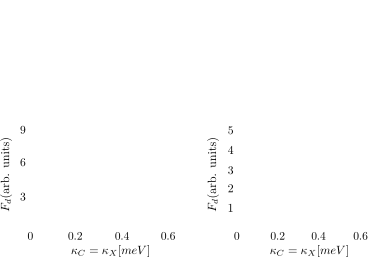
\includegraphics[width=.7\linewidth]{emiliano}
  \caption{
    % 
    \emph{Top row}: Photon density along $y=0$, perturbed by a
    circular potential of radius $7$ $\mu$m and height 110 meV (centered
    at the origin), in the subcritical regime. The pump momentum is $k_p =
    1$ $\mu$m${}^{-1}$, and the panels (from left to right) correspond to
    decreasing exciton ($\gamma_X$) and photon ($\gamma_C$) decay rates
    $\gamma_X = \gamma_C =$ 1.3, 0.44 and 0.011 meV. 
    % 0.6582119/(x [ps]) = \gamma/2 [meV]
    %
    \emph{Bottom row}: Residual drag force as a function of decay
    rate. The left panel compares two different values of $k_p$, namely
    0.7 (black solid line) and 1 $\mu$m${}^{-1}$ (red dashed line). The
    right panel shows two different potential heights, of -22 (blue
    dashed line) and -2.2 meV (red dashed line), with $k_p = 0.7$
    $\mu$m${}^{-1}$.
    %
    In all plots, the pump is 0.44 meV blue-detuned above the bare LP
    branch $\omega_{LP}(\kv_{p})$. Adapted from
    Ref.~\cite{Cancellieri_2010}.
    % 
  }\label{fig:emiliano}
\end{figure}

In the case of \emph{gapped} spectra, the situation is, however,
qualitatively different (see Fig.~\ref{fig:dragv}(a)). For infinitely
living polaritons, $\gamma \to 0$, the drag force can also be
evaluated analytically and its expression is similar to
Eq.~\eqref{eq:drag0}, but with a critical velocity larger than the
speed of sound, the expression of which is given in
Eq.~\eqref{eq:criti}:
%
\begin{equation}
  \frac{F_d}{(m\sub{LP}c_s)^3 g_V^2/g_X}=\frac{(v_p/c_s)^2 - 1}{v_p/c_s}
  \Theta(v_p - v^c)\; .
\end{equation}
%
Therefore now the drag experiences a jump for $v_p=v^c$, rather than a
continuous threshold as for the resonant case $\Delta_p=0$. As already
mentioned in the previous section, this discontinuous behaviour of the
drag for the gapped spectra is connected to the fact that, as soon as
quasiparticles can be excited by the defect at $v_p\ge v^c$,
Cherenkov-like waves can be immediately emitted in all directions,
rather than being restricted in a region outside the Mach cone as
before. For $\Delta_p=0$, the cone was gradually closing with
increasing  fluid velocity.

Both the increase of the value of the drag in the subcritical region
as a function of the polariton lifetime and the decrease in the
supercritical region, are behaviours common to all the types of
spectra. We plot the drag force as a function of $\gamma$ in
Fig.~\ref{fig:dragk}, for two values of the fluid velocity $v_p$ and a
specific value of the pump detuning $\Delta_p$, though we have checked
that the following results are generic. For $v_p < v^c$, we find that
the residual drag is a finite-lifetime effect only and, well below the
critical velocity, the drag force goes linearly to zero for
$\gamma \to 0$. This is in agreement with the results of
Ref.~\cite{Cancellieri_2010}, where the full GP equation for the
coupled exciton and photon fields was solved numerically for a
finite-size defect: see the bottom row of Fig.~\ref{fig:emiliano} for
the numerical drag in the limit of asymptotically large densities.

In the resonant case $\Delta_p=0$, the slope of the
drag for $v_p \ll c_s$ can be evaluated analytically starting from the
expression~\eqref{eq:dragf}:
%
\begin{equation*}
    \frac{F_d}{(m\sub{LP}c_s)^3 g_V^2/g_X} \mathop{\simeq}\limits_{\gamma \to 0} \frac{2 c_s}{\pi
      v_p} \left( \frac{1}{ \sqrt{1-(v_p/c_s)^2}} - 1 \right)
    \frac{\gamma}{2g_X |\psi_p|^2} \; .
\end{equation*}
%
The residual drag in the subsonic regime is an effect of the
broadening of the quasi-particles energies: Even when the spectrum
real part does not allow any scattering against the defect (e.g., for
$\Delta_p \le 0$), the broadening produces some scattering close to
the defect. This results in a perturbation of the fluid around the
defect, asymmetric in the direction of the fluid velocity (see panel
(a) of Fig.~\ref{fig:dragk}), similar to what was obtained in
Ref.~\cite{Cancellieri_2010} (see top row of
Fig.~\ref{fig:emiliano}). Instead, in the supersonic regime, the drag
force is weaker in the non-equilibrium case with respect to the
equilibrium one. This is caused by the finite lifetime tending to
suppress the propagation of the Cherenkov waves away from the defect,
as shown in panel (b) of Fig.~\ref{fig:dragk}.


\section{Conclusions and discussion}
\label{sec:concl}
%
To conclude, we have analysed the linear response to a weak defect of
resonantly pumped polaritons in the pump-only state, and we have been
able to determine two different kinds of threshold-like behaviours for
the drag force as a function of the fluid velocity. In the case of
either zero or positive pump detuning, one can continuously connect to
the case of equilibrium weakly interacting gases of
Chapter~\ref{cha:cold-gases}, where the drag displays a continuous
threshold with a critical velocity equal to the speed of
sound. However, for negative pump detuning, where the spectrum of
excitations is gapped, the drag shows a discontinuity with a critical
velocity larger than the speed of sound. In this sense, the case of
coherently driven microcavity polaritons in the pump-only
configuration displays a richer phenomenology than the case of
nonresonantly pumped polariton superfluids. We have also seen that the
absence of a long-range wake does not imply the absence of
dissipation, as a residual drag force due to the finite polariton
lifetime is always present in the system. In this sense, one can say
that we are not dealing with superfluid behaviour in a strict sense.

\begin{subappendices}
\section{GP equation for the LP branch}
\label{app:full}
%
If one starts from a description of polaritons in terms of separate
exciton and cavity photon fields, a rotation into the LP and UP basis,
followed by neglecting the occupancy of the upper polariton branch, as
explained in detail in Chapter~\ref{cha:polaritons}, results in the
following Gross-Pitaevskii equation (compare to
Eq.~\eqref{eq:mom-GPE}) for the LP field in momentum space
$\psi_{LP}(\bm{r},t) = \sum_{\bm{k}} e^{i\bm{k}\cdot \bm{r}}
\psi_{LP,\bm{k}} (t)$~\cite{Ciuti_2003}:
%
\begin{multline}
  i\partial_t \psi_{LP,\bm{k}} = f_p e^{-i\omega_p t}
  \delta_{\bm{k},\bm{k}_p} + \left[\omega_{LP} (\kv) - i\gamma
    (\kv)/2\right]\psi_{LP,\bm{k}} +\\
%
  \sum_{\bm{k}_1, \bm{k}_2} g_{\bm{k}, \bm{k}_1, \bm{k}_2}
  \psi^*_{LP,\bm{k}_1 + \bm{k}_2-\bm{k}} \psi_{LP,\bm{k}_1}
  \psi_{LP,\bm{k}_2} + C_{\kv} \sum_{\bm{k}_1} V_{d,{\bm{k} - \bm{k}_1}} \psi_{LP,\bm{k}_1} C_{\kv_1}\; ,
\end{multline}
%
where $\gamma(\kv)=\gamma_X X^2_{\kv} + \gamma_C C^2_{\kv}$ is the effective LP
decay rate,
%
\begin{equation}
  g_{\bm{k}, \bm{k}_1, \bm{k}_2}=g_X X_{\kv}X_{|\bm{k}_1 + \bm{k}_2-\bm{k}|} X_{\kv_1} X_{\kv_2}
\end{equation}
%
is the interaction strength, and where
$V_d(\bm{r}) = \sum_{\bm{k}} e^{i\bm{k}\cdot \bm{r}} V_{d,{\bm{k}}}$.

In these expressions, the coefficients (see Eqs.~\eqref{eq:hopfield-X}
and~\eqref{eq:hopfield-C}) 
%
\begin{equation}
  X^2_{\kv}, C^2_{\kv} = \frac{1}{2} \left(1 \pm \frac{\omega_C(\kv) -
    \omega_X(0)}{\sqrt{(\omega_C(\kv) - \omega_X(0))^2 +
      4\Omega_R^2}}\right)
\end{equation}
%
are the Hopfield coefficients used to diagonalise the free polariton
Hamiltonian. We want here to justify the simplified description done
in Eq.~\eqref{eq:basic}. If we follow the linear response expansion as
in~\eqref{eq:mfield}, the operator $\hat{\mathcal{L}}$ in momentum
space analogous to~\eqref{eq:opell} reads as:
%
\begin{equation}
  \mathcal{L}_{\bm{k},\bm{k}_p} = \begin{pmatrix}
    \widetilde{\omega_{LP}} (\delta \bm{k}+\bm{k}_p) - i
    \gamma(\delta \bm{k}+\bm{k}_p)/2 & g_X X_{\kv_p}^2 X_{\delta
      \bm{k}+\bm{k}_p} X_{\delta \bm{k}-\bm{k}_p} \psi_p^2
    \\ - g_X X_{\kv_p}^2 X_{\delta \bm{k}+\bm{k}_p} X_{\delta
      \bm{k}-\bm{k}_p}{\psi_p^{\star}}^2 & -
    \widetilde{\omega_{LP}}(\delta \bm{k}-\bm{k}_p) -
    i\gamma(\delta \bm{k}-\bm{k}_p)/2 \end{pmatrix}\; ,
\label{eq:opel2}
\end{equation}
%
where now $\widetilde{\omega_{LP}} (\delta \bm{k} \pm\bm{k}_p) =
\omega_{LP} (\delta \bm{k} \pm\bm{k}_p) -\omega_p + 2 g_X X_{\kv_p}^2
X_{\delta \bm{k} \pm \bm{k}_p}^2 |\psi_p|^2$. It is easy to show that
the eigenvalues of this operator coincide with our approximated
expressions~\eqref{eq:spect} in the limit of $\delta k \ll k_p$,
when $X_{\delta \bm{k} \pm \bm{k}_p}^2 \simeq X_{\kv_p}^2$, $C_{\delta
\bm{k} \pm \bm{k}_p}^2 \simeq C_{\kv_p}^2$ and when we can simply
rename $g_X \equiv g_X X_{\kv_p}^4$ and $\gamma \equiv
\gamma(\kv_p)$. It is interesting to note that, even if we would
retain the linear terms in $\bm{k}_p \cdot \delta \bm{k}$ in the
expansion of $X_{\delta \bm{k} \pm \bm{k}_p}^2$, this would result in
a renormalisation of the fluid velocity $\bm{v}_p$ in the
expression~\eqref{eq:spect} which takes into account the blue-shift of
the LP dispersion due to the interaction.
\end{subappendices}


%%% Local Variables:
%%% mode: latex
%%% TeX-master: "../thesis_berceanu"
%%% End:

%%%%%%%%%%%%%%%%%%%%%%%%%%%%%%%%%%%
% Key                | Occurences |
%--------------------+------------|
% Amo_2009 (*)       |          4 |
% Marchetti_2010     |          4 |
% Wouters_2007       |          4 |
% Wouters_2007_b     |          3 |
% Wouters_2010 (*)   |          3 |
%%%%%%%%%%%%%%%%%%%%%%%%%%%%%%%%%%%


\chapter{Polariton superfluidity in the OPO regime}
\label{cha:opo}

% TODO: As no restoring force opposes a global rotation of the
% signal-idler phases, the generator of such rotations is an
% eigenvector of L with eigenvalue 0.



\section{Introduction}
%
Microcavity polaritons, which are the quasiparticles resulting from
the coherent strong coupling between quantum well excitons and cavity
photons~\cite{9780199228942}, have unique mixed matter-light
properties that none of their constituents display on its own. Because
of their energy dispersion and their strong nonlinearity inherited
from the excitonic components, polaritons continuously injected by an
external laser into a pump state with suitable wavevector and energy
can undergo coherent stimulated scattering into two conjugate
states~\cite{Ciuti_2000,Ciuti_2001,Ciuti_2003}, namely the signal and
the idler, a process known as optical parametric oscillator (OPO).
%
Since their first
realisation~\cite{Stevenson_2000,Savvidis_2000,Savvidis_2000_b,Baumberg_2000,Saba_2001},
the interest in microcavity optical parametric phenomena has involved
several fields of fundamental and applicative
research~\cite{Edamatsu_2004,Savasta_2005,Lanco_2006,Abbarchi_2011,Ardizzone_2012,Xie_2012,Lecomte_2013}.

Recently, considerable resources have been invested in exploring the
fundamental properties of parametric processes, including the
possibility of macroscopic phase coherence and superfluid
behaviour~\cite{Carusotto_2013}.
%
In spite of the coherent nature of the driving laser pump, the OPO
process belongs to the class of non-equilibrium phase transitions in
which a $U(1)$ phase symmetry is spontaneously
broken~\cite{Wouters_2007}.
%
While the phase of the pumped mode is locked to the incident laser,
the phases of the signal and idler are free to be simultaneously rotated in
opposite directions.
%
Because of this phase freedom, recent experiments~\cite{Sanvitto_2010}
have tested the OPO superfluid properties by exploring the physics of
the signal-idler order parameter, demonstrating the existence and
metastability of vortex configurations. As the order parameter
involves both signal and idler, their phase windings have opposite
signs~\cite{Sanvitto_2010,Marchetti_2010,9783642241857}.  Crucially, this
causes both OPO fluids to display quantized flow metastability
simultaneously.

While in equilibrium condensates different aspects of superfluidity
are typically closely related~\cite{Leggett_1999}, this is no longer
true in a non-equilibrium context such as for microcavity
polaritons~\cite{Carusotto_2013}.
%
In particular, those aspects of superfluidity related to 
frictionless flow around defects are expected to be much more involved
in OPO condensates than for any other investigated polariton
condensates, such as for the case of incoherent
pumping~\cite{Kasprzak_2006,Wouters_2010}, and single-state
resonantly pumped microcavities~\cite{Amo_2009}.
%
Independent of the pumping scheme, the driving and the polariton
finite lifetime prompt questions about the meaning of superfluid
behaviour, when the spectrum of collective excitations is complex
rather than real, raising conceptual interrogatives about the
applicability of a Landau criterion~\cite{Wouters_2010}.
%
However, an additional complexity characterises the OPO regime, i.e., the
simultaneous presence of three oscillation frequencies and momenta for
pump, signal and idler correspondingly multiplies the number of
collective excitation branches~\cite{Wouters_2007}.
%
Note that from the experimental point of view, pioneering
experiments~\cite{Amo_2009_b} have observed a ballistic nonspreading
propagation of signal/idler polariton wavepackets in a triggered-OPO
configuration.
%
However, given the complexity of the dynamics as well as the nonlinear
interactions involved in this time-dependent
configuration~\cite{Szyma_ska_2010}, a theoretical understanding of these
observations is not yet complete.

This Chapter presents a joint theoretical and experimental study of an
OPO configuration where a wide and steady-state condensate hits a
stationary localized defect in the microcavity.
%
Contrary to the criterion for quantized flow metastability for which the
signal and idler display simultaneous locked responses, we find that
their scattering properties when the OPO hits a static defect are
different.
%
In particular we investigate the scattering properties of all three
fluids, the pump, the signal and the idler, in both real and momentum space. We
find that the modulations generated by the defect in each fluid are
not only determined by its associated Rayleigh scattering ring, but
each component displays additional rings because of the cross-talk
with the other components imposed by nonlinear and parametric
processes.
%
We single out three factors determining which one of these rings
has the biggest influence on each fluid response: the coupling strength between
the three OPO states, the resonance of the ring with the blue-shifted
LP dispersion, and the values of each fluid group velocity
and lifetime together establishing how far each modulation can
propagate from the defect.
%
The concurrence of these effects implies that the idler strongly
scatters, inheriting the same modulations as the pump, while the
modulations due to its own ring can propagate only very close to the
defect and cannot be appreciated. However, the modulations in the signal
are strongly suppressed, and not at all visible in experiments,
because the slope of the polariton dispersion in its low momentum
component brings all Rayleigh rings coming from pump and idler out of
resonance.

Note that the kinematic conditions for OPO are incompatible with the
pump and idler being in the subsonic regime. Thus, the coupling
between the three components always implies some degree of scattering
in the signal. In practice, the small value of the signal momentum
strongly suppresses its visible modulations, as confirmed by the
experimental observations.

\section{Model}
\label{sec:model-opo}

The dynamics of polaritons in the OPO regime and their hydrodynamic
properties when scattering against a defect can be described via a
classical driven-dissipative non-linear Gross-Pitaevskii equation
(GPE) for the coupled exciton and cavity fields $\psi_{X,C}
(\vt{r},t)$~\cite{Whittaker_2005,Carusotto_2013}:
%
\begin{equation}
  i\partial_t \begin{pmatrix} \psi_X \\ \psi_C \end{pmatrix} =
  \hat{H} \begin{pmatrix} \psi_X \\ \psi_C \end{pmatrix}
  + \begin{pmatrix} 0 \\ F_p(\vt{r},t) \end{pmatrix} \; .
\label{eq:gpequ}
\end{equation}
%
The dispersive $X$- and $C$-fields decay at a rate $\gamma_{X,C}$ and
are coupled by the Rabi splitting $\Omega_R$, while the nonlinearity
is regulated by the exciton coupling strength $g_X$:
%
\begin{equation}
  \hat{H} = \begin{pmatrix} \omega^{X}(-i\nabla) - i
    \frac{\gamma_X}{2} + g_X |\psi_X|^2 & \Omega_R/2 \\ \Omega_R/2 &
    \omega^C(-i\nabla) - i \frac{\gamma_C}{2} + V_d \end{pmatrix} \;
  .
\end{equation}
%
We describe the defect via a potential $V_d (\vt{r})$ acting on the
photonic component; this can either be a defect in the cavity mirror
or a localized laser field~\cite{Amo_2009,Amo_2010,Zajac_2012}.
%
In the conservative, homogeneous, and linear regime [$\gamma_{X,C}=0=
V_d (\vt{r})= g_X$], the eigenvalues of $\hat{H}$ are given by the
LP and UP energies, $2
\omega_{\vt{k}}^{LP,UP} = \omega_{\vt{k}}^{C} +
\omega_{\vt{k}}^{X} \mp \sqrt{(\omega_{\vt{k}}^{C} -
  \omega_{\vt{k}}^{X})^2 + \Omega_R^2}$.
%
The cavity is driven by a continuous-wave laser field $F_p(\vt{r},t)
= \mathcal{F}_p(\vt{r}) e^{i (\vt{k}_p \cdot \vt{r} - \omega_p
  t)}$ into the OPO regime: Here, polaritons are continuously injected
into the pump state with frequency $\omega_p$ and momentum
$\vt{k}_p$, and, above a pump strength threshold, they undergo coherent
stimulated scattering into the signal $(\omega_s, \vt{k}_s)$ and
idler $(\omega_i, \vt{k}_i)$ states. 

As a first step, it is useful to get insight into the system behaviour
in the simple case of a homogeneous pump of strength
$\mathcal{F}_p(\vt{r}) = f_p$. A numerical study of the coupled
equations~\eqref{eq:gpequ} for the more realistic case of a
finite-size top-hat pump profile $\mathcal{F}_p(\vt{r})$ will be
presented later.
%
To further simplify our analysis, we assume here that the UP
dispersion does not get populated by parametric scattering processes
and thus, by means of the Hopfield coefficients $2X_{\vt{k}}^2,
2C_{\vt{k}}^2 = 1 \pm (\omega_{\vt{k}}^{C} -
\omega_{\vt{k}}^{X})/\sqrt{(\omega_{\vt{k}}^{C} -
  \omega_{\vt{k}}^{X})^2 + \Omega_R^2}$, we project the
GPE~\eqref{eq:gpequ} onto the LP
component~\cite{Ciuti_2001,Wouters_2007_b} $\psi_{\vt{k}}^{} =
X_{\vt{k}} \psi_{X,\vt{k}} + C_{\vt{k}} \psi_{C,\vt{k}}$,
where $\psi(\vt{r},t) = \sum_{\vt{k}} e^{i\vt{k}\cdot \vt{r}}
\psi_{\vt{k}}^{} (t)$:
%
\begin{multline}
  i\partial_t \psi_{\vt{k}}^{} = \left[\omega_{\vt{k}}^{LP} -
    i\frac{\gamma_{\vt{k}}}{2}\right]\psi_{\vt{k}}^{} +
  C_{\vt{k}} \sum_{\vt{q}} C_{\vt{q}} V_d(\vt{k} - \vt{q})
  \psi_{\vt{q}}^{}\\ + \sum_{\vt{k}_1, \vt{k}_2} g_{\vt{k},
    \vt{k}_1, \vt{k}_2} \psi^*_{\vt{k}_1 + \vt{k}_2-\vt{k}}
  \psi_{\vt{k}_1}^{} \psi_{\vt{k}_2}^{} + \tilde{f}_p(t)
  \delta_{\vt{k},\vt{k}_p}\; .
\label{eq:efflp}
\end{multline}
%
Here, $\gamma_{\vt{k}}=\gamma_X X_{\vt{k}}^2 + \gamma_C C_{\vt{k}}^2$
is the effective LP decay rate, the interaction strength is given by
$g_{\vt{k}, \vt{k}_1, \vt{k}_2}=g_X X_{\vt{k}} X_{\vt{k}_1 +
  \vt{k}_2-\vt{k}} X_{\vt{k}_1} X_{\vt{k}_2}$, and the pumping term is
given by $\tilde{f}_p(t)= C_{\vt{k}_p} f_p e^{-i\omega_p t}$. Note
that the problematic dependence on the exciton-exciton interaction
strength $g_X$ can be removed by rescaling both the LP field
$\sqrt{g_X}\psi_{\kv}(t) \rightarrow \psi_{\kv}(t)$ and the pump
strength $\sqrt{g_X}f_p \rightarrow f_p$, something we will do later
on to all effects, working in terms of energy blueshifts and the
rescaled pump intensity.
%
\begin{figure}[tb]
\centering
\includegraphics[width=.9\linewidth]{3d0_0} % ~/notebooks/OPODrag/opodrag.py
\caption{OPO mean-field blueshifts and fluctuation
  Rayleigh rings in the linear-response scheme for homogeneous
  pumping. Left panel: signal $s$ ([blue] upper triangles), pump $p$
  ([red] circles), and idler $i$ ([green] lower triangles) mean-field
  energy blueshifts $\epsilon_{n=s,p,i}$ (in units of $\gamma_p =
  \gamma_{\vt{k}_p}$) vs the rescaled pump intensity $I_p$ (in
  units of $\gamma_p^3$) in the optical limiter regime. Parameters are
  $\Omega_R=5$~meV, zero cavity-exciton detuning, $\gamma_X = \gamma_C
  = 0.12$~meV, $\omega_p - \omega_0^X = -1.25$~meV, $k_p=1.6{\mu
    m}^{-1}$, $k_s \simeq 0$, and $k_i=3.2{\mu m}^{-1}$.  The shaded
  area is stable OPO region, while the vertical dashed line
  corresponds to the pump power value chosen for plotting the right
  panel. Right panel: blueshifted LP dispersion~\eqref{eq:blues} with
  superimposed Rayleigh curves $\Gamma_{p,i,(u,v), \tilde{\vt{k}} +
    \vt{k}_{p, i}}$ evaluated within the linear-response
  approximation (same symbols as left panel). The two rings
  corresponding to the signal state, $\Gamma_{s,(u,v),
    \tilde{\vt{k}}}$, are shrunk to zero because $k_s \simeq 0$.}
\label{fig:spect}
\end{figure}
%


\section{Linear-response theory}
\label{sec:line-resp-theory}
In the limit where the homogeneously pumped system is only weakly
perturbed by the external potential $V_d(\vt{r})$, we apply a
linear-response analysis~\cite{Astrakharchik_2004}: The LP field is
expanded around the mean-field terms for the three $n=1,2,3=s,p,i$ OPO
states~\cite{Whittaker_2005},
%
\begin{equation}
  \psi_{\tilde{\vt{k}}}^{} = \sum_{n=1}^3 e^{-i \omega_n t}
  \left[\psi_{n}^{} \delta_{\tilde{\vt{k}},0} +
    u_{n,\tilde{\vt{k}}}^{} e^{-i\omega t} +
    v^*_{n,-\tilde{\vt{k}}} e^{i\omega t} \right]\; ,
\label{eq:expan}
\end{equation}
%
where $\tilde{\vt{k}} = \vt{k} - \vt{k}_n$. Eq.~\eqref{eq:efflp}
is expanded linearly in both the fluctuation terms,
$u_{n,\tilde{\vt{k}}}^{}$ and $v_{n,\tilde{\vt{k}}}^{}$, as well
as the defect potential.  At zeroth order, the three complex uniform
mean-field equations can be solved to obtain the dependence of the
signal, pump and idler energy blueshifts, $\epsilon_n = g_X
X^2_{\vt{k}_n} |\psi_{n}^{}|^2$ on the system
parameters~\cite{Wouters_2007_b}. A typical behaviour of
$\epsilon_n$ as a function of the rescaled pump intensity $I_p = g_X
C_{\vt{k}_p}^2 f_p^2/X_{\vt{k}_p}^2$ in the optical limiter regime
is plotted in the left panel of Fig.~\ref{fig:spect}.
%
At first order, one obtains six coupled equations diagonal in momentum
space~\cite{Wouters_2007}
%
\begin{equation}
  \omega \vt{w}_{\tilde{\vt{k}}} = \mathcal{L}_{\tilde{\vt{k}}}
  \vt{w}_{\tilde{\vt{k}}} + \frac{1}{2} \bm{\Psi}_d\; ,
\label{eq:fluct}
\end{equation}
%
for the six-component vector $\vt{w}_{\tilde{\vt{k}}} =
(u_{n,\tilde{\vt{k}}}^{} , v_{n,\tilde{\vt{k}}}^{})^{T}$ and for
the potential part, $\bm{\Psi}_d = (\psi_n^{} C_{\vt{k}_n}
C_{\vt{k} + \vt{k}_n} V_d(\vt{k}),-\psi_n^* C_{\vt{k}_n}
C_{\vt{k}_n - \vt{k}} V_d(-\vt{k}))^{T}$. In ~\eqref{eq:fluct}
we have only kept the terms oscillating at the frequencies $\omega_n
\pm \omega$ and neglected the other terms in the expansion (i.e.,
$2\omega_n - \omega_m \pm \omega$), which are oscillating at
frequencies far from the LP band, and thus with negligible amplitudes.
%
In the particlelike and the holelike channels, the Bogoliubov matrix
determining the spectrum of excitations can be written
as~\cite{Wouters_2007}
%
\begin{equation}\label{eq:bogoliubov-opo}
  \mathcal{L}_{\vt{k}} = \begin{pmatrix} M_{\vt{k}}^{} & Q_{\vt{k}}^{}
    \\ -Q_{-\vt{k}}^* & -M_{-\vt{k}}^* \end{pmatrix} \; ,
\end{equation}
%
where the three OPO states components are
%
\begin{align}
  (M_{\vt{k}}^{})_{mn} &= \left[\omega^{LP}_{\vt{k}_m + \vt{k}}
    - \omega_m - i\frac{\gamma_{\vt{k}_m + \vt{k}}}{2}\right]
  \delta_{m,n} \\
%
  \nonumber & + 2\sum_{q,t=1}^3
  g_{\vt{k}_m+\vt{k},\vt{k}_n+\vt{k},\vt{k}_t} \psi_q^*
  \psi_t^{} \delta_{m+q,n+t}\\
%
  (Q_{\vt{k}}^{})_{mn} &= \sum_{q,t=1}^3
  g_{\vt{k}_m+\vt{k},\vt{k}_q,\vt{k}_t} \psi_q^{} \psi_t^{}
  \delta_{m+n,q+t}\; .
\end{align}
%
\begin{figure}[tb]
\centering
\includegraphics[width=.5\linewidth]{ks0_0}
% ~/notebooks/julia/april/linresp_waves.ipynb
% ~/notebooks/OPODrag/opodrag.py
\caption{Linear responses to a static defect of the three OPO states
  in real and momentum space. Rescaled filtered OPO emissions (signal
  [top panels], pump [middle], and idler [bottom]) in real space
  $|\psi (\vt{r},\omega_n)|^2/|\psi_n|^2$ (left panels in linear
  scale) and momentum space $|\psi_{\tilde{\vt{k}}} (\omega_n)|^2$
  (right panel in logarithmic scale) obtained within the
  linear-response approximation. The OPO parameters are the same ones
  in Fig.~\ref{fig:spect}, and the strength of the $\delta$-like
  defect potential, $V_d(\kv) = g_d$, is fixed to
  $g_d = 0.5 \gamma_p~\mu$m$^2$. For the top left panel of the signal
  emission in real space, Gaussian filtering is applied to enhance the
  short wavelength modulations, the amplitudes of which are otherwise
  roughly $1\%$ of the average signal intensity and about a factor of
  10 times weaker than the modulation amplitudes in the pump fluid.}
\label{fig:ereal}
\end{figure}
%

In absence of a defect potential ($\bm{\Psi}_d =0$),
Eq.~\eqref{eq:fluct} is the eigenvalue equation for the spectrum of
excitations of a homogeneous OPO, i.e.,
$\det(\mathcal{L}_{\tilde{\vt{k}}} - \omega)=0$. The spectrum has six
branches, $\omega_{n,(u,v),\tilde{\vt{k}}}$, labeled by $n=s,p,i$
and $(u,v)$. Even though these degrees of freedom are mixed together,
at large momenta, one recovers the LP dispersions shifted by the three
states' energies and momenta, i.e.,
%
\begin{equation}
  \lim_{\tilde{k} \gg \sqrt{2m_C \Omega_R}} \omega_{n,(u,v),\tilde{\vt{k}}} = \pm
  (\omega^{LP}_{\vt{k} - \vt{k}_n} - \omega_n)\; ,
\label{eq:large}
\end{equation}
%
where $+$ ($-$) corresponds to the $u$ ($v$) particlelike (holelike)
branch.
%
The OPO solution is stable (shaded area in Fig.~\ref{fig:spect}) as
far as $\Im[\omega_{n,(u,v),\tilde{\vt{k}}}] < 0$.

The shape of the patterns, or Cherenkov-like waves, resulting from the
elastic scattering of the OPO 3-fluids against the static ($\omega=0$)
defect can be determined starting from the spectrum, and in particular
evaluating the closed curves $\Gamma_{n,(u,v), \tilde{\vt{k}}}$ in
$\vt{k}$-space, or ``Rayleigh rings''~\cite{9783319002651} defined by
the condition $\Re[\omega_{n,(u,v), \tilde{\vt{k}}}] = 0$. Even if
they do not appear to be relevant here, note that the presence of a
non-vanishing imaginary part of the excitation spectrum
$\Im[\omega_{n,(u,v),\tilde{\vt{k}}}]\neq 0$ introduces some
complications: Even in the absence of any Rayleigh ring, the drag
force can be non-vanishing and the standard Landau criterion may fail
to identify a critical velocity~\cite{Wouters_2010}.
%
The modulations propagate with a direction
$\hat{\eta}_{n,(u,v),\tilde{\vt{k}}}$ orthogonal to each curve
$\Gamma_{n,(u,v), \tilde{\vt{k}}}$, a pattern wavelength given by
the corresponding $|\tilde{\vt{k}}|$, and a group velocity
$\vt{v}_{n,(u,v),\tilde{\vt{k}}}^{(g)}=\nabla_{\tilde{\vt{k}}}
\Re[\omega_{n,(u,v), \tilde{\vt{k}}}]$, where
$\xi_{n,(u,v),\tilde{\vt{k}}} =
|\vt{v}_{n,(u,v),\tilde{\vt{k}}}^{(g)} / \Im[\omega_{n,(u,v),
  \tilde{\vt{k}}}]|$ determines the distance, at any given direction
$\hat{\eta}_{n,(u,v),\tilde{\vt{k}}}$, over which the perturbation
extends away from the defect. For a single fluid under a coherent
pump, the qualitative shape of the modulation pattern generated in the
fluid by the defect is mostly determined by the excitation
spectrum~\cite{Carusotto_2006,Carusotto_2004}.

For OPO, the spectrum of excitation on top of each of the three,
$n=1,2,3$, states (see appendix~\ref{app:SM}) generates six identical
Rayleigh rings $\Gamma_{n,(u,v), \tilde{\vt{k}}}$ for the three states.
%
The Rayleigh rings for the OPO conditions specified in
Fig.~\ref{fig:spect} are clearly visible in the right panels of
Fig.~\ref{fig:ereal}, where we plot the $\vt{k}$-space
photoluminescence filtered at the energy of each state, i.e.,
$|\psi_{\tilde{\vt{k}}} (\omega_n)|^2= |\psi_{n}^{}
\delta_{\tilde{\vt{k}},0} + u_{n,\tilde{\vt{k}}}^{} +
v^*_{n,-\tilde{\vt{k}}}|^2$.
%
We have chosen here a $\delta$-like defect potential, $V_d(\vt{k}) =
g_d$, but we have  checked that our results do not depend on
its exact shape (see appendix~\ref{app:SM}).
%
For the OPO conditions considered here, the signal momentum is at $k_s
\simeq 0$, and thus only four of the six rings are present. The same
rings are also plotted in the right panel of Fig.~\ref{fig:spect},
shifted at each of the three OPO states' momentum $\vt{k}_n$,
$\Gamma_{n,(u,v), \tilde{\vt{k}}+\vt{k}_n}$ and energies
$\omega_n$.
%
It is important to note that, even though the three OPO states have
locked responses because they display the same spectrum of
excitations, only one of the rings $\Gamma_{n,(u,v),
  \tilde{\vt{k}}+\vt{k}_n}$ is the most resonant at $\omega_n$
with the interaction blueshifted LP dispersion,
%
\begin{equation}
  \bar{\omega}_{\vt{k}}^{LP} = \omega_{\vt{k}}^{LP} + 2 
  X_{\vt{k}}^2 \sum_{n=1}^3  \epsilon_n\; ,
\label{eq:blues}
\end{equation}
%
where $\epsilon_n = g_X X_{\vt{k}_n}^2 |\psi_n^{}|^2$ are the
mean-field energy blueshifts (measured in Fig.~\ref{fig:spect} in
units of $\gamma_p = \gamma_{\vt{k}_p}$).  This implies that the
most visible modulation for each fluid should be the most resonant
one, with superimposed weaker modulations coming from the other two
state rings.

In the specific case of Fig.~\ref{fig:spect}, the signal is at $k_s
\simeq 0$ and thus produces no rings in momentum space. The other four
rings are very far from being resonant with the blueshifted LP
dispersion~\eqref{eq:blues} at $\omega_s$, and thus the signal
displays only an extremely weak modulation coming from the next
closer ring, which is the one associated with the pump state,
$\Gamma_{p,u, \tilde{\vt{k}}+\vt{k}_s}$.
%
We estimate that the signal modulation amplitudes are roughly $1\%$ of
the average signal intensity and about a factor of 10 times weaker
than the modulation amplitudes in the pump fluid.
%
To show that the signal has weak modulations coming from
the pump, we apply a Gaussian filter to the real space images (see the
inset of the top-left panel of Fig.~\ref{fig:ereal}).
%
As explained in more detail in appendix~\ref{app:SM}, Gaussian
filtering consists of subtracting from the original data a copy that
has been convoluted with a Gaussian kernel, thus getting rid of the
long-wavelength modulations.
%
This procedure reveals that indeed the pump imprints its modulations
also into the signal, even though these are extremely weak, thus
leaving the signal basically insensitive to the presence of the
defect.

Pump and idler states are each mostly resonant with their own
rings, i.e., $\Gamma_{p,u, \tilde{\vt{k}}+\vt{k}_p}$ at $\omega_p$
and $\Gamma_{i,u, \tilde{\vt{k}}+\vt{k}_i}$ at $\omega_i$,
respectively. Thus one should then observe two superimposed
modulations in both pump and idler filtered emissions, the stronger
one for each being the most resonant one.
%
However, the modulations associated with the idler only propagate very
close to the defect, at an average distance
$\overline{\xi_{i,u,\tilde{\vt{k}}}} \sim 1.7~\mu$m before getting
damped, and thus are not clearly visible. For the OPO conditions
considered, this is due to the small idler group velocity
$\vt{v}_{i,u,\tilde{\vt{k}}}^{(g)}$, as the dispersion is almost
excitonic at the idler energy.

We can conclude that, for the typical OPO condition with a signal at
$k_s \simeq 0$, considered in Figs.~\ref{fig:spect}
and~\ref{fig:ereal}, the signal fluid does not show modulations and
the extremely weak scattering inherited from the pump state can be
appreciated only after a Gaussian filtering procedure of the image. In
contrast, the idler has a locked response to the one of the pump
state.
%
Note that, for the conditions shown in Fig.~\ref{fig:spect}, as well
as the other cases considered in appendix~\ref{app:SM}, the subsonic to
supersonic crossover of the pump-only state~\cite{Amo_2009} happens
well above the region of stability of OPO. Thus it is not possible to
study a case where the pump is already subsonic and at the same time
promotes stimulated scattering.


\section{Experiments}
%
\begin{figure}[tb]\centering
  \includegraphics[width=.5\linewidth]{exp_waves}
  % ~/notebooks/julia/april/extract_exp_waves.ipynb
  \caption{Experimental OPO spectrum (lower panel) and filtered
    emissions of signal (top), pump (middle), and idler (bottom) in
    presence of a structural defect. The six panels show the filtered
    emission profiles in real space $I_{s, p,i}(\vt{r})$. A Gaussian
    filtering to enhance the short wavelength modulations is applied
    in the right column. The extracted wave crests from the idler
    (yellow contours in the bottom panel) are also superimposed on the
    pump profile (middle) by applying a $\pi$ phase-shift.}
\label{fig:exper}
\end{figure}
%
%
\begin{figure}[tb]
\centering
\includegraphics[width=.5\linewidth]{GP_space_mom}
% ~/Development/gp-linear-response/filtering-theory-GP.py
% ~/notebooks/julia/april/GP_signal_inset.ipynb
\caption{Full numerical responses to a static defect of
  the three OPO states in real and momentum space. Filtered OPO
  emissions (signal [top panels], pump [middle], and idler [bottom])
  in real space $|\psi_C (\vt{r},\omega_n)|^2$ (left panels in
  linear scale) and momentum space $|\psi_C
  (\tilde{\vt{k}},\omega_n)|^2$ (right panel in logarithmic scale)
  obtained by a full numerical evaluation of~\eqref{eq:gpequ}. For the
  top left panel of the signal space emission, Gaussian filtering is
  applied to enhance the short wavelength modulations of this state,
  revealing that the modulations corresponding to the pump state are
  also imprinted (though weakly) into the signal. The symbols indicate
  the pump ring diameter extracted from fitting the upstream
  modulations and resulting in a density-wave wavevector coinciding
  with that of the pump, $k_p=1.6$~$\mu$m$^{-1}$.}
\label{fig:numer}
\end{figure}
%
We now turn to the experimental analysis, where a continuous-wave
laser is used to drive a high quality ($Q=14000$) GaAs microcavity
sample into the OPO regime --- details on the sample can be found in
Refs.~\cite{Ballarini_2013,Dominici_2014}.
%%
The polariton dispersion is characterised by a Rabi splitting
$\Omega_R=5.4$~meV and the exciton energy is
$\omega_0^{X}=1485.26$~meV, while the cavity-exciton detuning is
slightly negative, $-1$~meV. The pump is at $k_p=0.89~\mu$m$^{-1}$ and
$\omega_p - \omega_0^{X}=-2.43$~meV, and, at pump powers $1.5$-times
above threshold, an OPO appears, with signal at small wavevector
$k_s=0.21~\mu$m$^{-1}$ and $\omega_s - \omega_0^{X}=-2.95$~meV, and
idler at $k_i=1.57~\mu$m$^{-1}$ and
$\omega_i - \omega_0^{X}=-1.91$~meV.
%
The defect used in the sample is a localized inhomogeneity naturally
present in the cavity mirror. Note that the exact location of the
defect can be extracted from the emission spectrum and is indicated
with a dot (orange) symbol in the profiles of Fig.~\ref{fig:exper}.

To filter the emission at the three states' energies,
$I_{s,p,i}(\vt{r}=x,y)$, and to obtain 2D spatial maps for the three
OPO states, one uses a spectrometer and, at a fixed position $x_0$,
one obtains the intensity emission as a function of energy and
position, $I(\epsilon,x_0,y)$. By changing $x_0$ one can build the
full emission spectrum as a function of energy and 2D position,
$I(\epsilon,\vt{r})$. The filtered emission for each OPO state is
obtained from the integrals
$I_{n=s,p,i}(\vt{r}) = \int_{\omega_n-\sigma}^{\omega_n+\sigma}
d\epsilon I(\epsilon, \vt{r})$, with $\sigma=0.08$~meV. The results
are shown in Fig.~\ref{fig:exper} for, respectively, the signal (top
panel), pump (middle) and the idler (bottom) profiles. Energy and
momentum of the three OPO states are labeled with a [blue] upper
triangle (signal), a [red] circle (pump), and a [green] lower triangle
(idler), while the localised state, clearly visible just below the
bottom of the LP dispersion, is indicated with the symbol $d$. The
bare LP dispersion is extracted from an off-resonant low pump power
measurement, as well as the emission of the exciton reservoir (X) and
that of the UP dispersion (each in a different scale).
%
The signal profile shows no appreciable modulations around the defect
locations, nor could any  be observed after applying a Gaussian
filtering procedure of the image.
%
In contrast, in agreement with the theoretical results, both filtered
profiles of the pump and idler show the same Cherenkov-like pattern. We
extracted the wave crests from the idler profile ([yellow] contours in
the bottom panel) and superimposed them on the pump profile (middle
panel) with an added $\pi$ phase-shift, revealing that the only
modulations visible in the idler state are the ones coming from the
pump state.


\section{Numerical analysis}
\label{sec:numerical-analysis}
%
The agreement between the results obtained experimentally and within
the linear-response approximation is additionally confirmed by an
exact full numerical analysis of the coupled
equations~\eqref{eq:gpequ} for a finite size pump via a
5$^{\text{th}}$-order adaptive-step Runge-Kutta algorithm.
%
Details are given in appendix~\ref{app:SM}.
%
The pumping conditions are very similar to those previously considered
in the linear-response approximation of Figs.~\ref{fig:spect}
and~\ref{fig:ereal}, while the pump profile $\mathcal{F}_p(\vt{r})$ is
now a finite-size top hat. In particular, we consider the case of zero
cavity-exciton detuning, $k_p=1.6$~$\mu$m$^{-1}$,
$\omega_p-\omega_X^0 = -0.44$~meV and the pump power strength is fixed
just above threshold, such as to produce a stable steady state OPO.
This, in absence of the defect, is characterized by a signal at small
wavevector $k_s=-0.2$~$\mu$m$^{-1}$ and idler at
$k_i=3.4$~$\mu$m$^{-1}$.

When adding a localised defect potential, the steady state OPO
develops Rayleigh rings in momentum space, yet, as shown in appendix~\ref{app:SM},
the spectrum continues to be $\delta$-like in energy, allowing us to
easily filter in energy the emission of the three OPO states.
%
Results are shown in Fig.~\ref{fig:numer}, where real-space emissions
$|\psi_C (\vt{r},\omega_n)|^2$ are plotted in the left panels, while
the ones in momentum space $|\psi_C (\tilde{\vt{k}},\omega_n)|^2$ are
plotted in the right panels. We observe a very similar phenomenology
to that one obtained in the linear approximation shown in
Fig.~\ref{fig:ereal}. The signal now is at slightly negative values of
momenta $k_s=-0.2$~$\mu$m$^{-1}$, thus implying a very small Rayleigh
ring associated with this state. Thus we observe that only the
modulations associated with the pump are the ones that are weakly
imprinted in the signal state and that can be observed by means of a
Gaussian filtering (inset of the top-left panel). We have fitted the
upstream wave crests and obtained the same modulation wavevector as
the pump one ([blue] upper triangles). Similar to the linear-response
case, we also find here that the most visible perturbation in the
emission filtered at the idler energy is the one due to the pump
Rayleigh ring. As before, the modulations due to the idler Rayleigh
ring cannot propagate far from the defect because of the small group
velocity associated with this state.


\section{Conclusions}
%
To conclude, we have presented a joint theoretical and experimental
study of the superfluid properties of a nonequilibrium condensate of
polaritons in the so-called optical parametric oscillator
configuration by studying the scattering against a static defect.
%
We have found that, while the signal is basically free from
modulations, the pump and idler lock to the same response. We have
highlighted the role of the coupling between the OPO components due to
nonlinear and parametric processes. These are responsible for the
transfer of the spatial modulations from one component to the
other. This process is most visible in the clear spatial modulation
pattern that is induced by the nonsuperfluid pump onto the idler,
while the same modulations are only extremely weakly transferred into
the signal, because of its low characteristic wavevector, so much that
experimentally cannot be resolved.
%
The main features of the real- and momentum-space emission patterns
are understood in terms of Rayleigh scattering rings for each
component and a characteristic propagation length from the defect; the
rings are then transferred to the other components by nonlinear and
parametric processes.

Much interest has been recently devoted to aspects related to
algebraic order~\cite{Altman_2015,PhysRevX.5.041028} and superfluid
response~\cite{Keeling_2011_prl} in drive-dissipative polariton
condensates. Our theoretical and experimental results further stress
the complexities and richness involved when looking for superfluid
behavior in nonequilibrium multicomponent condensates such as the ones
obtained in the OPO regime.


\begin{subappendices}
\section{Signal state at nonzero momenta}
\label{app:SM}
%
\begin{figure}[tb]\centering
\includegraphics[width=.9\linewidth]{GP_disp}
% ~/notebooks/julia/theory-GP.ipynb
\caption{OPO spectrum obtained by full numerics. Left
  panel: Photonic component of the OPO spectrum in presence of a
  point-like defect, $|\psi_C(k_x,0,\omega)|^2$ (logarithmic scale),
  as a function of the rescaled energy $\omega - \omega_0^X$ versus
  the $x$-component of momentum $k_x$ (cut at $k_y=0$) for a top-hat
  pump (see text for the space profile and parameter values), with
  intensity $f_p=1.23 f_p^{\text{th}}$ above the OPO threshold, pump
  wave-vector $k_p=1.6$~$\mu$m$^{-1}$ in the $x$-direction and
  $\omega_p-\omega_X^0=-0.44$~meV. The symbols indicate the signal
  ([blue] upper triangle), pump ([red] circle), and idler ([green]
  lower triangle) energies, as well as the two momenta $k_x$ on each
  state Rayleigh ring at $k_y=0$. Note that the logarithmic scale
  results in a fictitious broadening in energy of the spectrum, which
  is in reality $\delta$-like (see right panel). The bare LP
  dispersion, including its broadening due to finite lifetime, is
  plotted as a shaded grey region, while the bare UP dispersion as a
  (black) dot-dashed line. Right panel: Momentum integrated spectrum,
  $\sum_{\vt{k}} |\psi_C(\vt{k},\omega)|^2$ (linear scale) as a
  function of the rescaled energy $\omega - \omega_0^X$, where it can
  be clearly appreciated that the emission is $\delta$-like in
  energy.}
\label{fig:spectGP}
\end{figure}
%
In Chapter~\ref{cha:opo}, we presented a theoretical and experimental
analysis of the response of microcavity polaritons in the OPO regime
to a static defect.
%
For the theoretical calculations we follow two independent approaches:
In the first approach, we exactly numerically solve the dynamics of
the two coupled Gross-Pitaevskii equations (GPEs) for the exciton and
cavity fields for the realistic case of a finite-size top-hat pump
profile $\mathcal{F}_p(\vt{r})$. In the second approach, we apply a
perturbative linear-response approximation for the LP
LP state, which leads to semi-analytical results in the limiting case
of a spatially homogeneous pump profile. Both methods have been
already successfully used in the literature to explore several
properties of the OPO operation.

While all fundamental formulae and information has been given in the
Chapter text, in this appendix we present some additional details on
both approaches that might be of interest to the specialized reader.
In addition to that, we make use of the linear-response approach to
examine some regimes that are hardly accessed experimentally or within
a full numerical approach.


\subsection{Full numerics}
\label{subsec:detun}
The classical driven-dissipative non-linear Gross-Pitaevskii equation
(GPE) for the coupled exciton and cavity fields $\psi_{X,C}
(\vt{r},t)$
%
\begin{equation}
  i\partial_t \begin{pmatrix} \psi_X \\ \psi_C \end{pmatrix} =
  \hat{H} \begin{pmatrix} \psi_X \\ \psi_C \end{pmatrix}
  + \begin{pmatrix} 0 \\ F_p(\vt{r},t) \end{pmatrix}\; ,
\label{eq:numer}
\end{equation}
%
where
%
\begin{equation}
  \hat{H} = \begin{pmatrix} \omega^{X}(-i\nabla) - i
    \frac{\gamma_X}{2} + g_X |\psi_X|^2 & \Omega_R/2 \\ \Omega_R/2 &
    \omega^C(-i\nabla) - i \frac{\gamma_C}{2} + V_d \end{pmatrix} \;
  ,
\end{equation}
%
is solved numerically on a 2D grid of $N\times N=2^8\times 2^8$ points
and a separation of $0.47$~$\mu$m (i.e., in a box $L\times L =
121$~$\mu$m$\times 121$~$\mu$m) by using a 5$^{\text{th}}$-order
adaptive-step Runge-Kutta algorithm. Convergence has been checked both
with respect the resolution in space $L/N$ as well as in momentum
$\pi/L$, without~\cite{Marchetti_2010,9783642241857} as well as in
presence of the defect.
%
The same approach has been already used in the literature, for a
review, see Refs.~\cite{Marchetti_2010,9783642241857}).
%
As for the system parameters, we have considered a LP dispersion at
zero photon-exciton detuning, $\omega^C_0 = \omega^X_0$, a
dispersionless excitonic spectrum, $\omega^X_{\vt{k}} = \omega^X_0$
and a quadratic dispersion for photons $\omega^C_{\vt{k}} =
\omega^C_0 + k^2/2m_C$, with the photon mass $m_C=2.3 \times 10^{-5}
m_e$, where $m_e$ is the bare electron mass. The LP dispersion, $2
\omega_{\vt{k}}^{LP} = \omega_{\vt{k}}^{C} + \omega_{\vt{k}}^{X}
- \sqrt{(\omega_{\vt{k}}^{C} - \omega_{\vt{k}}^{X})^2 +
  \Omega_R^2}$ is characterised by a Rabi splitting $\Omega_R =
4.4$~meV. Furthermore, the exciton and cavity decay rates are fixed to
$\gamma_X=\gamma_C=0.53$~meV.
%
For the defect we choose a $\delta$-like potential
%
\begin{equation}
  V_d(\vt{r}) = g_d \delta(\vt{r} - \vt{r}_0)\; ,
\end{equation}
%
where its location $\vt{r}_0$ is fixed at one of the $N \times N$
points of the grid.
%
Note that in a finite-size OPO, local currents lead to inhomogeneous
OPO profiles inside the pump spot, despite the external pump having
a top-hat profile with a completely flat inner
region~\cite{Marchetti_2010,9783642241857} --- as shown later, this
can be observed in the filtered OPO profiles evaluated in absence of a
defect, shown as dashed lines in Fig.~\ref{fig:rafull}.
%
We have thus chosen the defect location so that it lies in the
smoothest and most homogeneous part of the OPO profiles.
%
\begin{figure}[tb]\centering
\includegraphics[width=.5\linewidth]{rangesGP.png}
% ~/Development/gp-linear-response/filtering-theory-GP.py
\caption{Real space signal, pump and idler OPO one-dimensional
  filtered profiles derived from finite size numerics with and without
  a defect. Rescaled OPO filtered emissions along the $y=0$ direction,
  $|\psi_C(x,y=0,\omega_n)|^2 \frac{\Omega_R}{2g_X}$, obtained by
  numerically solving the GPE Eq.~\eqref{eq:gpequ} of
  Sec.~\ref{sec:model-opo}. While the dashed lines represent the
  filtered emissions of signal (top panel), pump (middle) and idler
  (bottom) for a top-hat pump without a defect, the solid lines are
  the same OPO conditions but now for a defect positioned at
  $(x_d, y_d) = (9.5, -0.5)$~$\mu$m corresponding to the vertical
  dotted lines. The system parameters are the same ones as those of
  Fig.~\ref{fig:numer}.}
\label{fig:rafull}
\end{figure}
%

Also we have checked that our results do not qualitatively depend on
the strength $g_d$ (nor on the sign) of the defect potential, as far
as this does not exceed a critical value above which it destabilises
the OPO steady-state regime.
%
The pump, $F_p(\vt{r},t) = \mathcal{F}_p(\vt{r}) e^{i (\vt{k}_p
  \cdot \vt{r} - \omega_p t)}$, has a smoothen and rotationally
symmetric top-hat profile, $\mathcal{F}_p(\vt{r}) = \mathcal{F}_p(r)
= \frac{f_p}{2}[\tanh(\frac{r+\sigma_p}{r_0}) -
  \tanh(\frac{r-\sigma_p}{r_0})]$ with strength $f_p = 1.23
f_p^\text{th} = 0.053$~meV/$\mu$m and parameters $r_0 = 8.68~\mu$m,
$\sigma_p = 34.72~\mu$m.
%
We pump at $k_p=1.6$~$\mu$m$^{-1}$ in the $x$-direction, $\vt{k}_p =
(k_p,0)$, and at $\omega_p-\omega_X^0=-0.44$~meV, i.e., roughly
$0.5$~meV above the bare LP dispersion. By increasing the pump
strength $f_p$, we find the threshold $f_p^{\text{th}}$ above which
OPO switches on, leading to two conjugate signal and idler states.
%
We then fix the pump strength just above this threshold ($f_p=1.23
f_p^{\text{th}}$), where we find a steady state OPO solution which is
stable (see Ref.~\cite{9783642241857} for further details). In
absence of the defect, this condition corresponds to a signal state at
$k_s=-0.2$~$\mu$m$^{-1}$ and $\omega_s-\omega_0^X = -1.64$~meV and an
idler at $k_i=3.4$~$\mu$m$^{-1}$ and $\omega_i-\omega_0^X =
0.76$~meV. 
%
It is interesting to note that already very close to the lower pump
power threshold for OPO, the selected signal momentum is very close to
zero. This contrasts with what one obtains in the linear approximation
scheme, where instead just above the lower OPO threshold there exists
a broad interval of permitted values for $k_s$ (and thus $k_i$) --- we
will further discuss this ``selection problem'' for parametric
scattering in Sec.~\ref{subsec:analy}.

We evaluate the time dependent full numerical solution
of~\eqref{eq:numer} $\psi_{X,C} (\vt{r},t)$, until a steady state
regime is reached. Here, both its Fourier transform to momentum
$\vt{k}$ and energies $\omega$ can be evaluated numerically.
%
We plot on the left panel of Fig.~\ref{fig:spectGP} a cut at $k_y=0$
of the photonic component of the OPO spectrum in presence of a
point-like defect, $|\psi_C(k_x,0,\omega)|^2$, as a function of the
rescaled energy $\omega - \omega_0^X$ versus the $x$-component of
momentum $k_x$ (cut at $k_y=0$). In the right panel we plot instead
the corresponding momentum integrated spectrum, $\sum_{\vt{k}}
|\psi_C(\vt{k},\omega)|^2$.
%
Here, we can clearly see that the presence of the defect does not
modify the fact that the OPO emission for the OPO signal ([blue] upper
triangle), pump ([red] circle), and idler ([green] lower triangle)
states has a completely flat dispersion in energy, thus indicating
that a stable steady state OPO solution has been reached. Note that in
the spectrum map of the left panel of Fig.~\ref{fig:spect}, the
logarithmic scale results in a fictitious broadening in
energy. However, from the integrated spectrum plotted in linear scale
in the right panel of Fig.~\ref{fig:spect} one can clearly appreciate
that this emission is $\delta$-like, exactly as it happens for the
homogeneous OPO case~\cite{9783642241857}.
%
Thus the effect of the defect is to induce only elastic (i.e., at the
same energy) scattering; now the three OPO states emit each on its own
Rayleigh ring (given each by the symbols on the left panel of
Fig.~\ref{fig:spectGP} which represent the rings at a cut for
$k_y=0$). This makes it rather difficult to extract the separated
signal, pump and idler profiles by filtering in momentum, as done
previously for the homogeneous case, but it still allows to filter
those profiles very efficiently in energy. In fact, because the
emission is $\delta$-like, it is enough to fix a single value of the
energy $\omega$ to the one of the three states $\omega_{n=s,p,i}$,
thus extracting the filtered profiles either in real space
$|\psi_C(\vt{r},\omega_n)|^2$ or in momentum space
$|\psi_C(\vt{k},\omega_n)|^2$ --- we have however checked that
integrating in a narrow energy window around $\omega_n$ does not
quantitatively change the results.

The results of the above described filtering are shown in
Fig.~\ref{fig:numer}.
%
In Fig.~\ref{fig:rafull} we instead plot the corresponding
one-dimensional profiles in the $y=0$ direction both in presence
(solid line) and without (dashed line) a defect. Here, we can observe
that, even if the pump has a top-hat flat profile, as also commented
previously, in absence of a defect, the finite-size OPO is
characterised by inhomogeneous profiles of signal, pump and idler
because of localised currents. Further, we observe that the presence
of a defect induces strong modulations in pump and idler.
%
In order to reveal that the pump also imprints its modulation into the
signal, even though these are extremely weak (and hardly visible in
both the top main panel of Fig.~\ref{fig:numer} and the top panel of
Fig.~\ref{fig:rafull}), we apply a Gaussian filtering to the signal
images, the result of which is shown in the inset of the top-left
panel of Fig.~\ref{fig:numer}.
%
This consists of the following procedure. The original data for the
real space profile $\psi(\vt{r})$ are convoluted with a Gaussian
kernel $K(\vt{r} - \vt{r}')$, obtaining a new profile,
$\tilde{\psi}(\vt{r}') = \int d\vt{r} \psi (\vt{r}) K(\vt{r} -
\vt{r}')$, where short wavelengths features are smoothened out. The
convoluted image $\tilde{\psi}(\vt{r}')$ is then subtracted from the
original data, giving $\psi(\vt{r}) - \tilde{\psi}(\vt{r})$, and
effectively filtering out all long wavelength details.
%
The same procedure of Gaussian filtering is also applied to the signal
emission profile obtained within the linear-response analysis and
shown in the inset of the top left panel of Fig.~\ref{fig:ereal}.

%
\begin{figure}[tb]\centering
\includegraphics[width=.7\linewidth]{fig_excitation_ks_0_000.png}
% ~/notebooks/OPODrag/opodrag.py
\caption{Spectrum of collective excitations. Cut at $k_y=0$ of the
  real part of the quasiparticle energy dispersion
  $\Re [\omega_{n,(u,v),\vt{k}-\vt{k}_n}]$ plotted versus $k_x -
  k_n$. The spectrum is evaluated within the linear approximation
  scheme and the parameters are the same ones used for
  Fig.~\ref{fig:ereal}.}
\label{fig:bogol}
\end{figure}
%
%
\begin{figure}[tb]
\centering
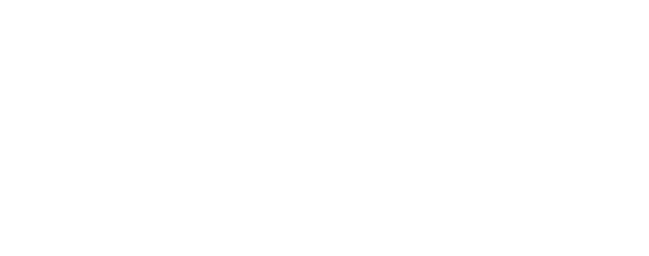
\includegraphics[width=.5\linewidth]{3d0_7.png}
\includegraphics[width=.5\linewidth]{ks0_7.png}
% ~/notebooks/OPODrag/opodrag.py
\caption{OPO for finite and positive signal momentum in the
  linear-response approximation for homogeneous pumping. Rescaled OPO
  emission within the linear-response approximation in real
  $|\psi (\vt{r},\omega_n)|^2/|\psi_n|^2$ (left panels in linear
  scale) and momentum space $|\psi_{\tilde{\vt{k}}} (\omega_n)|^2$
  (right panels in linear scale) filtered at the energies of the three
  OPO states: signal (top panels), pump (middle), and idler
  (bottom). The parameters are the same as those used in
  Fig.~\ref{fig:ereal}, with the exception of the signal and idler
  momenta, which are now at $k_s = 0.7$~$\mu$m$^{-1}$ and
  $k_i = 2.5$~$\mu$m$^{-1}$ respectively. Each scale of variation for
  the profiles is plotted in the color-box next to the left panels. A
  cut in the $y=0$ direction for the three profiles is plotted in the
  bottom panel of Fig.~\ref{fig:range}.}
\label{fig:ksp07}
\end{figure}
%
%
\begin{figure}[tb]
\centering
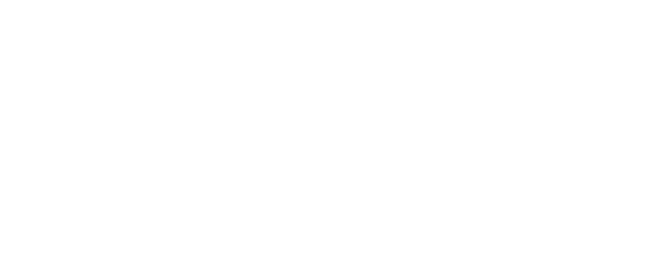
\includegraphics[width=.5\linewidth]{3d-0_4.png}
\includegraphics[width=.5\linewidth]{ks-0_4.png}
% ~/notebooks/OPODrag/opodrag.py
\caption{OPO for finite and negative signal momentum in the
  linear-response approximation for homogeneous pumping. Rescaled OPO
  emission within the linear-response approximation in real
  $|\psi (\vt{r},\omega_n)|^2/|\psi_n|^2$ (left panels in linear
  scale) and momentum space $|\psi_{\tilde{\vt{k}}} (\omega_n)|^2$
  (right panels in linear scale) filtered at the energies of the three
  OPO states: signal (top panels), pump (middle), and idler
  (bottom). The parameters are the same as those used in
  Fig.~\ref{fig:ereal}, with the exception of the signal and idler
  momenta, which are now at $k_s = -0.4$~$\mu$m$^{-1}$ and
  $k_i = 3.6$~$\mu$m$^{-1}$ respectively. A cut in the $y=0$ direction
  for the three profiles is plotted in the top panel of
  Fig.~\ref{fig:range}.}
\label{fig:ksm04}
\end{figure}
%
\begin{figure}[tb]\centering
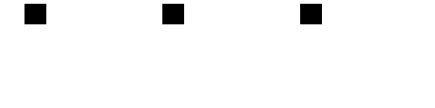
\includegraphics[width=.5\linewidth]{ranges.png}
% ~/notebooks/OPODrag/opodrag.py
\caption{Real space signal, pump and idler OPO one-dimensional
  filtered profiles in the linear-response approximation. OPO filtered
  emissions along the $y=0$ direction,
  $I (x, y=0, \omega_n) = |\psi(x,y=0, \omega_n)|^2/|\psi_n|^2$.  A
  signal at $k_s = -0.4$~$\mu$m$^{-1}$ (top panel) corresponds to
  Fig.~\ref{fig:ksm04}, a signal at $k_s = 0.0$~$\mu$m$^{-1}$ (middle
  panel) corresponds to Fig.~\ref{fig:ereal}, and a signal at
  $k_s = 0.7$~$\mu$m$^{-1}$ (bottom panel) corresponds to
  Fig.~\ref{fig:ksp07}. In each panel we plot the filtered profiles of
  signal, pump, and idler, while the horizontal gray dashed lines
  represent the values of the mean-field emission without a defect.}
\label{fig:range}
\end{figure}
%
\begin{figure}[tb]\centering
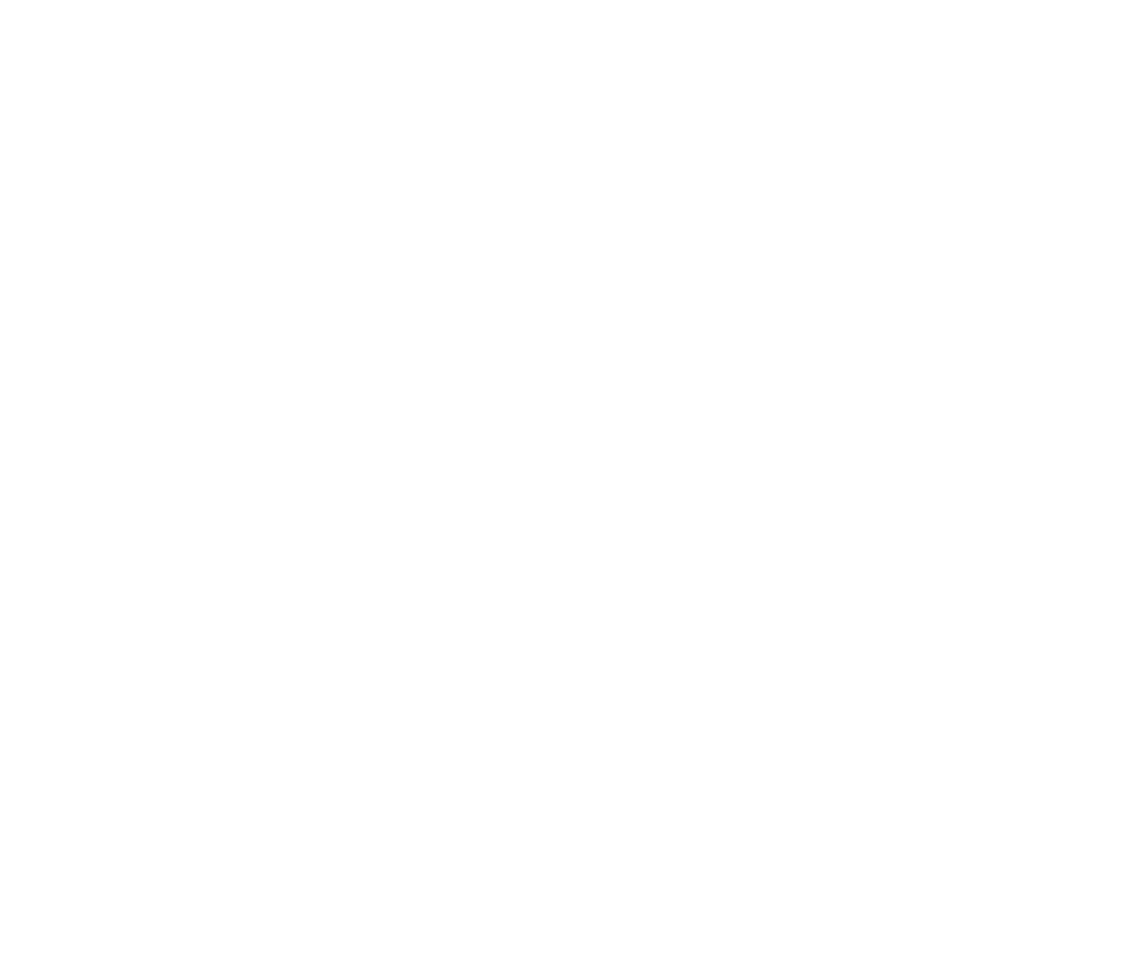
\includegraphics[width=.8\linewidth]{uncoupled.png}
% ~/notebooks/OPODrag/opodrag.py
\caption{Real space profiles of three uncoupled signal, pump and idler
  fluids. The rescaled profiles
  $|\psi (\vt{r},\omega_n)|^2/|\psi_n|^2$ are obtained by setting all
  off-diagonal couplings in Eq.~\eqref{eq:bogoliubov-opo} to zero,
  resulting in three uncoupled signal (left column), pump (middle
  column), and idler (right column) fluids. The three rows correspond
  to the three different cases previously analysed within the
  linear-response approximation: the case of a signal at
  $k_s = -0.4$~$\mu$m$^{-1}$ (top row) corresponds to the same
  conditions as Fig.~\ref{fig:ksm04}, a signal at
  $k_s = 0.0$~$\mu$m$^{-1}$ (middle row) corresponds to
  Fig.~\ref{fig:ereal}, and a signal at $k_s = 0.7$~$\mu$m$^{-1}$
  (bottom row) corresponds to Fig.~\ref{fig:ksp07}.}
\label{fig:uncou}
\end{figure}
%


\subsection{Linear response}
\label{subsec:analy}
%
In Chapter~\ref{cha:opo}, we also made use of the linear-response
approximation to analyse the OPO response to a static defect, valid
for a homogeneous pumping scheme. In order to do so, we first
evaluated the Bogoliubov matrix given in
Eq.~\eqref{eq:bogoliubov-opo}, whose eigenvalues determine the
spectrum of collective excitations. We plot in Fig.~\ref{fig:bogol} a
typical collective dispersion (here we consider the same system
parameters as the ones used in Fig.~\ref{fig:ereal}), by plotting the
real part of the Bogoliubov matrix eigenvalues
$\Re[\omega_{n,(u,v),\vt{k}-\vt{k}_n}]$ as a function of $k_x - k_n$
(cut at $k_y=0$). Note that the Rayleigh rings can be found by finding
the intersections $\Re[\omega_{n,(u,v),\vt{k}-\vt{k}_n}]=0$.

As also done for the full numerics, we consider a $\delta$-like
disorder potential $V_d(\vt{r}) = g_d \delta(\vt{r} - \vt{r}_0)$, and
Figs.~\ref{fig:spect} and~\ref{fig:ereal}, as well as
Figs.~\ref{fig:ksp07} and~\ref{fig:ksm04} below, are plotted for this
case.
%
We have checked that our results do not depend on the specific shape
of the defect potential: In particular, we have also considered the
response to defects with smooth Gaussian-like profiles, whose effect
is only to partially weaken the upstream modulations in real space.

We have seen in Chapter~\ref{cha:opo} that both experimentally as well
as in the full numerical analysis, one obtains OPO conditions where
the signal momentum is very close to zero, $\vt{k}_s \sim 0$. The
reason why OPO selects almost zero momentum signal conditions is still
awaiting a theoretical explaination.
%
In contrast, the linear-response approximation allows to access very
different OPO mean-field conditions, for which, by leaving unaltered
the value of the pump momentum, the signal can appear at finite
momentum values, either positive or negative.
%
This is a peculiarity of this approximation scheme, where one can show
that, at mean-field level, one has the possibility of choosing
different values of the signal momentum $\vt{k}_s$ (and thus the one
of the idler $\vt{k}_i$), and that this choice range is quite broad
particularly when the pump power is close to the lower pump threshold
for OPO --- the stability region for OPO is plotted as a shaded grey
region in the top left panels of Figs.~\ref{fig:ksp07}
and~\ref{fig:ksm04}. This is a well known ``selection problem'' for
parametric scattering (see Ref.~\cite{Wouters_2007_b}): The reason why
in full numerical calculations, parametric scattering processes select
a signal with a momentum close to zero, already very close to the
lower pump thresold for OPO, is still awaiting an explaination. In
particular, this quest cannot be addressed within a spatially
homogeneous approximation where the three mean-field solutions for
pump, signal, and idler states can be describes by plane waves.
%%
One can only show that, within the same mean-field approximation
scheme, when increasing the pump power towards the upper threshold for
OPO, the blue-shift of the LP polariton dispersion due to the
increasing mean-field polariton density, causes the signal momentum to
converge towards zero~\cite{Whittaker_2005} $\vt{k}_s \rightarrow 0$.

{\em{OPO with finite momentum signal--}} Given the freedom of choice for
the signal momentum $\vt{k}_s$ close to the lower OPO threshold, we
consider here two additional cases, that could not be studied neither
experimentally, nor within a full numerical approach, but that instead
we can easily analize within the linear-response theory.
%
In particular, we have left fixed the pumping conditions
$k_p=1.6$~$\mu$m$^{-1}$ and $\omega_p-\omega_X^0=-1.25$~meV and
considered two opposite situations.

In the first case, the signal has a finite and positive momentum $k_s
= 0.7$~$\mu$m$^{-1}$ and thus the idler is at low momentum, $k_i
=2.5$~$\mu$m$^{-1}$. The results are shown in Fig.~\ref{fig:ksp07}.
%
Here we see that all six Rayleigh rings are clearly visible and, in
addition, as the idler is at lower momentum compared to the case
considered in Figs.~\ref{fig:spect} and~\ref{fig:ereal}, and thus its
dispersion steeper, the idler group velocity is large enough to
appreciate the modulation of the Rayleigh ring associated to this
state. As a result, each of the three filtered OPO emissions exhibits
as the strongest modulation the one coming from its own Rayleigh ring,
including the signal which is now at finite and large momentum. In this
case, the OPO response of each filtered state profile looks completely
independent from the other, as if we were pumping each state
independently.

In the second case, shown in Fig.~\ref{fig:ksm04}, the signal is
finite and negative, $k_s = -0.4$~$\mu$m$^{-1}$, and the idler is now
at very large momentum, $k_i = 3.6$~$\mu$m$^{-1}$, where its
dispersion is very exciton-like and flat, and thus the idler has a
very small group velocity and its own modulations are visible only
very close to the defect. For this case, we can appreciate in the
idler filtered profile overlapped modulations from all the three state
Rayleigh rings (note that because the signal is at negative momentum,
its modulations have an opposite direction compared to the ones of
pump and idler), while in the signal we can mostly see the signal long
wavelength modulations and only very weakly the pump one.

We can compare the different modulation strengths of the three OPO
profiles by looking at the color bars plotted next to the profiles. In
order to better compare them on the same plot, we show in
Fig.~\ref{fig:range} the one-dimensional OPO filtered emissions along
the $y=0$ direction, rescaled by the mean-field solution $\psi_n$ in
absence of the defect, for the three cases analysed above. While for
the OPO conditions with a signal at $k_s = 0.0$~$\mu$m$^{-1}$ (middle
panel, corresponding to Fig.~\ref{fig:ereal}), the imprinted
modulations from the pump are hardly visible, and can only be
appreciated after a Gaussian filter manipulation, both OPO cases with
a finite momentum signal result in modulations in the signal with an
amplitude of the same order of magnitude of both pump and idler
fluids.

In Fig.~\ref{fig:uncou} we instead show the real space profiles
obtained by setting all off-diagonal couplings in the Bogoliubov
matrix $\mathcal{L}_{\vt{k}}$ of Eq.~\eqref{eq:bogoliubov-opo} to
zero, resulting in three uncoupled signal (left column), pump (middle
column), and idler (right column) fluids. This underlines the
importance of the coupling between the three fluids in the three
different OPO regimes previously analysed within the linear-response
approximation. In particular, for the OPO conditions such that the
signal has a finite and positive momentum $\vt{k}_s$ (bottom row of
Fig.~\ref{fig:uncou}, which corresponds to the conditions shown in
Fig.~\ref{fig:ksp07}), the coupling has little effect and the three
fluids respond to the defect in practice in a independent way (each
Rayleigh ring influences its own fluid). The OPO condition with a
finite and negative momentum $\vt{k}_s$, which corresponds to the
conditions shown in Fig.~\ref{fig:ksm04}, are shown in the top row of
Fig.~\ref{fig:uncou}: Here, we can see that the coupling between the
three fluids plays a role. The modulations of the pump can be
appreciated both in the signal profile (though weakly), as well as in
the idler profile. In the idler fluid its own modulations can only
propagate very close to the defect and thus the only really
appreciable modulations are the ones inherited from the pump. Finally,
for the experimentally relevant case of an OPO with a signal at zero
momentum (middle row of Fig.~\ref{fig:uncou}, which corresponds to the
conditions shown in Fig.~\ref{fig:ereal}), there is also a role played
by the coupling, though, as already thoroughly analysed, the
modulations in the signal inhereted from the pump can only be
appreciated after a Gaussian filtering manipulation.


Finally note that, as it also happens for the OPO conditions shown in
Fig.~\ref{fig:spect} of this Chapter, the subsonic to supersonic
crossover of the pump-only state~\cite{Amo_2009} happens at pump
intensities well above the region of stability of OPO --- the shaded
gray regions of Figs.~\ref{fig:ksp07} and~\ref{fig:ksm04} Thus, it is
not possible to study a case where the pump is already subsonic and at
the same time promotes stimulated scattering.

\section{Source code}\label{sec:source-code-opo}
%
This appendix contains \textsc{Python} 2.7 source code used for the
linear-response formalism in Chapter~\ref{cha:opo}, resulting in
Figs.~\ref{fig:spect}, \ref{fig:ereal}, \ref{fig:bogol},
\ref{fig:ksp07}, \ref{fig:ksm04}, \ref{fig:range},
and~\ref{fig:uncou}. The figures are plotted using the
\textsc{matplotlib} library, and the 3 coupled nonlinear equations of
state describing the OPO regime are solved using \textsc{PHCpack}, a
general-purpose solver for polynomial systems by homotopy continuation
methods.
%
%%%%%%%%%%%%%%%%%%%%%%%%%%%%%%%%%%%%%%%%%%%%%%%%%%%%%%%%%%%
% pygmentize -l python -f latex -o opodrag.tex opodrag.py %
%%%%%%%%%%%%%%%%%%%%%%%%%%%%%%%%%%%%%%%%%%%%%%%%%%%%%%%%%%%


\subsection{opodrag.py}\label{subsec:opodrag}




%%% Local Variables:
%%% mode: latex
%%% TeX-master: "../../thesis_berceanu"
%%% End:

\end{subappendices}

%%% Local Variables:
%%% mode: latex
%%% TeX-master: "../thesis_berceanu"
%%% End:

%%%%%%%%%%%%%%%%%%%%%%%%%%%%%%%%%%%%%%%%%%%%
% Key                         | Occurences |
%-----------------------------+------------|
% price2014magnetic           |         14 |
% ozawa2014momhh              |          9 |
% hafezi2013imaging           |          7 |
%%%%%%%%%%%%%%%%%%%%%%%%%%%%%%%%%%%%%%%%%%%%

% TODO: add updates from Hannah's proceedings
% TODO: add Hannah's new figure(s) from proceedings
% TODO: cite conference proceedings .~\cite{proceeding}

\chapter{Landau levels in driven-dissipative cavity arrays}
\label{cha:landau}

In 1984, Michael Berry showed that the adiabatic evolution of energy
eigenfunctions with respect to a time-dependent Hamiltonian contains a
phase of geometrical origin, commonly known today by the name of
"Berry's phase" \cite{Berry_1984}.  Although Berry's seminal paper gave
the example of a spinor's evolution under slowly changing magnetic
field, geometric phases \cite{shapere1989geometric} with similar
origin have been encountered in a plethora of physical contexts,
ranging from hydrodynamics to quantum field theory, the quantum Hall
effect and topological insulators.

In a condensed matter context, the eigenstates of electrons in a
periodic lattice can be labeled by a band index $n$ and the crystal
momentum $\kv$. The Berry-phase physics arising when adiabatically
transitioning between neighbouring wavevectors was appreciated only
recently. This phenomenon can explain properties such as electric
polarization, anomalous Hall conductivity or the quantization of
conductance in the integer quantum Hall effect.

In the presence of a (synthetic) gauge field, the eigenstates making
up an energy band can have nontrivial geometrical properties, as
encoded in the Berry connection and Berry curvature~\cite{berry,
  xiao2010berryreview}. Understanding the geometry of eigenstates in a
band is of great importance, not least because the integral of the
Berry curvature over the 2D Brillouin zone (BZ) gives the first Chern
number: the topological invariant responsible for the integer quantum
Hall effect~\cite{thouless}. Consequently, there has been much work in
recent years to develop new techniques with which to probe the
properties of energy bands in photonics and ultracold gases. For
example, the Berry curvature can be measured in the semiclassical
dynamics of a wavepacket in an optical lattice~\cite{dudarev,1chang,
  price, cominotti, dauphin, aidelsburger2015measuring,
  jotzu2014experimental} or in photon transport in a cavity
array~\cite{ozawa2014qhe}. In all these cases, the physics can be most
naturally understood by recognising that the Berry curvature acts like
a magnetic field in momentum space~\cite{berry, bliokh2005spin,
  PhysRevD.12.3845, cooper2012designing}.

The analogy between Berry curvature and magnetism is most powerful
when a geometrical energy band is subjected to an additional weak
harmonic potential~\cite{price2014magnetic}. Then, in the effective
momentum-space Hamiltonian, a harmonic potential acts like the kinetic
energy of a particle in real space. Just as the physical momentum
$\vt{k}-\vt{A}(\rv)$ is the sum of the canonical momentum $\vt{k}$ and
the magnetic vector potential $\vt{A} (\rv)$ in the magnetic
Hamiltonian, so the physical position $\vt{r}+\mathcal{A}_{n,n}(\kv)$,
is given by the canonical position $\vt{r}$ and the Berry connection
$\mathcal{A}_{n,n}(\kv)$ of band $n$ in the effective
Hamiltonian~\cite{adams1959energy,nagaosa,
murakami2003dissipationless, bliokh2005spin, fujita,
bliokh2005topological,gosselin2006semiclassical}. The Berry curvature,
$\Omega_n (\kv)= \nabla \times \mathcal{A}_{n,n}(\kv)$, is then like a
momentum-space magnetic field. For certain models, this analogy leads
to a clear analytical understanding of single-particle
dynamics~\cite{price2014magnetic, ozawa2014momhh, price2015sporbit,
Claassen_prl_2015}. In particular, we will focus on the small-flux
limit of the Harper-Hofstadter
Hamiltonian~\cite{harper1955magnetic,hofstadter1976butterfly}, which
is a model that has recently been realized in a multitude of
experimental configurations, ranging from ultracold
gases~\cite{aidelsburger2013hh,miyake2013hh,mancini2015edge,stuhl2015edge},
solid state superlattices~\cite{dean2013hofstadter,yu2014hierarchy}
and silicon photonics~\cite{hafezi2013imaging} to classical systems
such as coupled pendula~\cite{susstrunk2015pendula} and oscillating
circuits~\cite{jia2013circuits}. As first shown in
Ref.~\cite{price2014magnetic}, the eigenstates of this model in the
presence of a harmonic trap are toroidal Landau levels in momentum
space. Not only would an observation of these states constitute the
first exploration of analogue magnetic states in momentum space, but
also the first experimental study of magnetism on a torus.
 
Most theoretical works on momentum-space Landau levels have focused on
conservative dynamics~\cite{price2014magnetic, Claassen_prl_2015},
while photonic systems naturally include driving and
dissipation~\cite{carusotto2013fluids}. In this Chapter, we present a
realistic experimental proposal for the observation of these states in
a driven-dissipative 2D lattice of cavities, such as the array of
coupled silicon ring resonators of Ref.~\cite{hafezi2013imaging},
where link resonators were used to simulate a synthetic gauge field
for photons. We combine this set-up with a harmonic potential,
introduced, for example, by a spatial modulation of the resonator
size. We demonstrate numerically that the main features of
momentum-space Landau levels will be observable spectroscopically in
this system for realistic parameters.

In this Chapter, we also emphasize how the inherent driving and
dissipation in photonics can be a key advantage in probing properties
that are otherwise inaccessible.  Firstly, the spectroscopic
measurements discussed here are sensitive to the absolute energy of a
state. From this, we show how to extract the energy shift due to the
off-diagonal matrix elements of the Berry connection
$\mathcal{A}_{n,n'}(\kv)$ relating eigenstates in different bands $n$
and $n'$. Only very recently has the first measurement of such effects
been reported in ultracold atomic
gases~\cite{Grusdt2014nonabelian,tracy2015arxiv}, and the approach
used in this experiment would be difficult to apply to a photonics
set-up. The scheme we present may therefore be useful for the
characterisation of energy bands in topologically-nontrivial photonic
systems.

Secondly, since the photon steady-state depends on the overlap between
the (observable) spatial amplitude profile of the drive and of the
eigenstates~\cite{carusotto2013fluids}, the observables will depend on
the phase of the eigenfunctions and thus on the specific synthetic
magnetic gauge that is implemented in a given experimental realization
of the Harper-Hofstadter Hamiltonian using a synthetic gauge field. We
note that a related gauge-sensitivity has also recently been of much
interest in ultracold gases in suitably designed time-of-flight
experiments~\cite{kennedy2015bec,spielman2011gauge, spielman_gauge,
tomoki2015nv}. Experiments on synthetic magnetic fields therefore
present the opportunity of straightforwardly probing gauge-dependent
physics.

This Chapter is organized as follows: in Section \ref{sec:model} we
add a harmonic trap to the HH model introduced in
Sec.~\ref{sec:hh-atoms}. We explain how the eigenstates can be
understood as momentum-space Landau levels in Section
\ref{sec:eigenstates}, before we discuss the breakdown of
approximations in Section \ref{sec:berry-shift}, focusing on the
energy shift from the off-diagonal matrix elements of the Berry
connection. Then in Section \ref{sec:driven-dissipation}, we add
driving and dissipation to the model. In Section \ref{sec:selection},
we show numerical results highlighting gauge-dependent effects, before
presenting a viable proposal for a photonics-based experiment in
Section \ref{sec:experiment}. Finally, we draw conclusions in Section
\ref{sec:conclusion}.


\section{The trapped Harper-Hofstadter Model}
\label{sec:model}

In this Chapter, we study the Harper-Hofstadter Hamiltonian
$\mathcal{H}_0$ in the presence of an external harmonic trap. The full
tight-binding Hamiltonian $\mathcal{H}$ of this system is
%
\begin{align} \mathcal{H} &= \mathcal{H}_0+\frac{1}{2}\kappa
\sum_{m,n}\left[(m-m_0)^{2}+(n-n_0)^{2}\right]\hat{a}_{m,n}^{\dagger}\hat{a}_{m,n} \label{eq:model}\\
\mathcal{H}_0 &= -J\sum_{m,n}(e^{i
\phi_{m,n}^x}\hat{a}_{m+1,n}^{\dagger}\hat{a}_{m,n} +e^{i
\phi_{m,n}^y}\hat{a}_{m,n+1}^{\dagger}\hat{a}_{m,n}) +
\text{H.c.} \label{eq:hh_hamiltonian}
\end{align}
%
where $J$ is the real hopping amplitude and $\hat{a}_{m,n}^{\dagger}$
($\hat{a}_{m,n}$) are the creation (annihilation) operators for a
particle on a square lattice at site $(m,n)$. The harmonic trap is of
strength $\kappa$ and is centered at a position $(m_0, n_0)$ which, in
general, need not coincide with a lattice site. Throughout, the
lattice spacing is set equal to one.

As explained in Sec.~\ref{sec:hh-atoms}, the hopping phases
$\phi = (\phi_{m,n}^x, \phi_{m,n}^y)$ are the Peierls phases gained by
a charged particle hopping in the presence of a perpendicular magnetic
field~\cite{harper1955magnetic,hofstadter1976butterfly}. The sum of
the phases around a square plaquette of the lattice is therefore equal
to $2\pi\alpha$, where $\alpha$ is the number of magnetic flux quanta
through the plaquette (with $\hbar=e=1$). For neutral particles, such
as photons, these phases can be imposed artificially to simulate the
effects of magnetism, for example, by inserting link resonators into
an array of silicon ring resonators as mentioned
above~\cite{hafezi2013imaging}.

Although the sum of phases around a plaquette is set by the external
(synthetic) flux, the exact form of the hopping phases themselves
depends on the choice of magnetic gauge. In the Landau gauge, for
example, $\phi = (0, 2\pi\alpha m)$ such that only the hopping
amplitude along one direction is modified. Conversely, in the
symmetric gauge, $\phi = (-\pi\alpha n, \pi\alpha m)$ and so hopping
terms along both $x$ and $y$ are affected, preserving the $C_4$
rotational invariance of the lattice. This gauge-dependence of the
hopping phases is reflected in the spatial profile of the phase of an
eigenstate of $\mathcal{H}$. In a photonics experiment, this phase is
an observable quantity as the intensity response of a system to a
given external driving is determined by the overlap of the spatial
amplitude distribution of the pump with the eigenstates. Such
experiments will therefore be sensitive to the synthetic magnetic
gauge as we discuss in Section \ref{sec:experiment}.

\subsection{Toroidal Landau Levels in Momentum
Space}\label{sec:eigenstates}

Having introduced the full Hamiltonian in Eq.~\eqref{eq:model}, we now
review how the eigenstates of this model in an appropriate limit can
be understood as toroidal Landau levels in momentum
space~\cite{price2014magnetic}. Throughout the following discussion,
we assume that the trap is centered at the origin $(m_0, n_0)= (0,0)$.

We begin from the eigenstates of the Harper-Hofstadter model
$\mathcal{H}_0\ket{\chi_{n,\vt{k}}} = E_n (\kv)
\ket{\chi_{n,\vt{k}}}$, where $E_n (\kv)$ is the energy dispersion of
band $n$ at crystal momentum $\vt{k}$. As the spatially-dependent
hopping phases in $\mathcal{H}_0$ break translational invariance, new
magnetic translation operators must be introduced to define a larger
magnetic unit cell, containing an integer number of magnetic flux
quanta~\cite{zak1964group, zak1964representations, 1chang}. Then
translational symmetry is restored and Bloch's theorem can be applied
to write the eigenstates as $\ket{\chi_{n,\vt{k}}} =
\frac{1}{\sqrt{N}} e^{i\vt{k}\cdot \vt{r}} \ket{u_{n,\vt{k}}}$, where
$\ket{u_{n,\vt{k}}}$ is the periodic Bloch function and $N$ is the
number of lattice sites. Thanks to the new larger unit cell, the
crystal momentum and the periodic Bloch functions here are defined in
the smaller magnetic Brillouin zone (MBZ). For example, hereafter, we
take the number of flux quanta per plaquette to be of the form
$\alpha=1/q$, where $q$ is an integer. Then the magnetic unit cell can
be chosen to be $q$ times larger than the original unit cell, while
the MBZ is $q$ times smaller than the original BZ.

Adding the harmonic trap breaks all translational symmetry of the
lattice, but we can use the eigenstates of $\mathcal{H}_0$ as a basis
in which to expand the new wave function $\ket{\psi} =
\sum_n\sum_{\vt{k}} \psi_n(\vt{k})
\ket{\chi_{n,\vt{k}}}$. Substituting this expansion into the full
Schr\"{o}dinger equation $i \partial_t \ket{\psi} = \mathcal{H}
\ket{\psi}$, it can be shown that the expansion coefficients
$\psi_n(\vt{k})$ satisfy~\cite{price2014magnetic}:
%
\begin{multline} i \partial_t \psi_n(\vt{k}) = E_n(\vt{k}) +
\frac{\kappa}{2}\sum_{n^{'},n^{''}}\left(\delta_{n,n^{'}}i
\nabla_{\vt{k}} + \mathcal{A}_{n,n^{'}}(\vt{k})\right)\times \\ \times
\left(\delta_{n^{'},n^{''}}i\nabla_{\vt{k}} +
\mathcal{A}_{n^{'},n^{''}}(\vt{k})\right) \psi_{n^{''}}(\vt{k}) \label{eq:first}
\end{multline} where $\mathcal{A}_{n,n^{'}}(\vt{k}) =
i\bra{u_{n,\vt{k}}}\nabla_{\vt{k}}\ket{u_{n^{'},\vt{k}}}$ is the
matrix-valued Berry connection.

To proceed, we consider the harmonic trap to be sufficiently weak
compared to the bandgap that we can make a single-band
approximation~\cite{price2014magnetic}. This assumes that only one
coefficient $\psi_n$ is non-negligible and that the external trap does
not significantly mix different energy bands. Then Eq.~\eqref{eq:first}
reduces to
%
\begin{equation} i \partial_t \psi_n(\vt{k}) = \widetilde{\mathcal{H}}
\psi_n(\vt{k})
\end{equation} where we have introduced the effective momentum-space
Hamiltonian
%
\begin{equation}\label{eq:dual} \widetilde{\mathcal{H}} =
\frac{\kappa}{2} [i\nabla_{\mathbf{k}} + \mathcal{A}_{n,
n}(\mathbf{k})]^2 + E_n(\mathbf{k}) + \frac{\kappa}{2}\sum_{n^{'}\neq
n} \abs{\mathcal{A}_{n,n^{'}}(\vt{k})}^2
\end{equation}
%
For the moment we focus on the first two terms; we discuss the role of
the last term, which comes from the off-diagonal matrix elements of
the Berry connection, in detail in the next subsection.  As can be
seen, there is a close analogy between the first two terms in the
momentum-space Hamiltonian and that of a charged particle in an
electromagnetic field {\em in real space}:
%
\begin{equation}\label{eq:mag} \mathcal{H}'=
\frac{\left[-i\nabla_{\vt{r}} - \vt{A}(\vt{r})\right]^2}{2M} +
\Phi(\rv)
\end{equation}
%
In this analogy, the role of the particle mass $M$ is played by
$\kappa^{-1}$, while the scalar potential $ \Phi(\rv)$ is replaced by
the energy band dispersion $E_n(\mathbf{k})$ and the magnetic vector
potential $\vt{A}(\vt{r})$ by the intra-band Berry connection
$\mathcal{A}_{n, n}(\mathbf{k})$. We note that both the magnetic
vector potential and the Berry connection are gauge-dependent
quantities. We hereafter refer to the gauge choice for the Berry
connection as the Berry gauge, and the gauge choice for a real-space
magnetic vector potential as the magnetic gauge. From the Berry
connection, we can also define the geometrical Berry curvature
$\Omega_{n}(\mathbf{k}) =\nabla \times \mathcal{A}_{n,
n}(\mathbf{k})$, which acts like a momentum-space magnetic field
$B(\vt{r})$.

The topology of momentum space also plays a crucial role here, as the
MBZ is topologically equivalent to a torus. One important consequence
of this is of course that the integral of Berry curvature over the
whole MBZ is quantised in units of the first Chern number
$\mathcal{C}_n$. In the above analogy with magnetism, this means that
the particle is confined to move on the surface of a torus, while the
Chern number counts the number of magnetic monopoles contained
inside~\cite{Fang}.

The above analogy with magnetism is particularly powerful because
there are natural limits for our model Eq.~\eqref{eq:model} in which the
eigenstates of Eq.~\eqref{eq:mag} and hence of Eq.~\eqref{eq:dual} are
known analytically~\cite{price2014magnetic, ozawa2014momhh,
Claassen_prl_2015}. We will focus on the flat-band limit in which the
bandwidth is much smaller than the trapping energy; for the energy
bands of $\mathcal{H}_0$ with $\alpha = 1/q$, this assumption improves
as $\kappa$ decreases or as $q$ increases. In this limit, we can
firstly approximate $\Omega_{n}(\mathbf{k}) \approx \Omega_n$, so that
the first term is analogous to the kinetic energy of a particle in a
uniform magnetic field. Secondly, we can approximate $E_n(\vt{k})
\approx E_n$ so that the second term of $\widetilde{\mathcal{H}}$ is
just a constant energy shift. Hence, the corresponding eigenstates can
be understood as toroidal Landau levels in momentum space. We note
that the opposite limit, in which the trapping energy is small
compared to the bandwidth, also yields very interesting physics
including the realisation of a Harper-Hofstatder model in momentum
space~\cite{ozawa2014momhh, scaffidi2014exact}.

As shown in Ref.~\cite{price2014magnetic}, the momentum-space toroidal
Landau levels form semi-infinite ladders of states:
%
\begin{equation}\label{eq:ladders} \epsilon_{n,\beta} = E_n +
\left(\beta + \frac{1}{2}\right) \kappa |\Omega_n|
\end{equation} where we have introduced the Landau level quantum
number~\cite{Landau:101810} $\beta = 0,1,2,\dots$, and where $\kappa
|\Omega_n|$ can be
recognised as the analogue of the cyclotron frequency $\omega_c = e
|B| /M $. Again, we note that here we have neglected the contribution
from the last term in Eq.~\eqref{eq:dual}, as this will be discussed in
the next subsection. As can be shown from the Diophantine equation for
the Hall conductivity, for odd values of $q$, the Chern number of all
bands except the middle band is $\mathcal{C}_n =
-1$~\cite{bernevig2013topological}. Then as the Chern number is
related to the uniform Berry curvature as $\mathcal{C}_n = (1/2\pi)
\Omega_n A_{\text{MBZ}}$, where $A_{\text{MBZ}} = (2\pi)^2/q$ is the
MBZ area, the Berry curvature is given by $|\Omega_n| =
\frac{1}{2\pi\alpha}$~\cite{price2014magnetic}.

While the above spectrum does not directly depend on the toroidal
topology of momentum space, the topology does enter into the
eigenstate degeneracy, which is equal to $|\mathcal{C}_n|$, as well as
into the analytical form of the eigenstates in the MBZ. For example,
for the bands with $\mathcal{C}_n = -1$, the eigenstates can be
written as~\cite{price2014magnetic}
%
\begin{align}\label{eq:chi}
\begin{split} \chi_\beta (\vt{k}) &= \mathcal{N}_\beta^{l_{\Omega_n}}
\sum_{j = - \infty}^{\infty} e^{- i k_y j } e^{ - ( k_x + j
l_{\Omega_n}^2 ) ^2 / 2 l_{\Omega_n}^2}\\ &\quad \times H_\beta ( k_x
/ l_{\Omega_n} + j l_{\Omega_n})
\end{split}\\ \mathcal{N}_\beta^{l_{\Omega_n}} &= \left(
\frac{\sqrt{2/q}} {2^\beta\beta! \times 2 \pi l_{\Omega_n}^2}
\right)^{1/2}
\end{align}
% 
where $H_\beta$ are the Hermite polynomials and $l_{\Omega_n} =
\sqrt{1/|\Omega_n|}$ is the analogue of the magnetic length. Here we
have taken the Berry gauge to have a Landau form
$\mathcal{A}_n(\mathbf{k}) = \Omega_n k_x \hat{\vt{k}}_y$ parallel to
the $\hat{\vt{k}}_y$ unit vector in momentum space. We have also
assumed that the MBZ is of length $2 \pi$ in one momentum direction,
and $2 \pi / q$ in the other direction, corresponding to a magnetic
unit cell of $q$ plaquettes containing one flux quantum. While this
choice of MBZ is valid in any magnetic gauge of the underlying
Harper-Hofstadter model, it is particularly natural when the hopping
phases in $\mathcal{H}_0$ are in the Landau magnetic gauge $\phi = (0,
2\pi\alpha m)$, as we shall discuss further below.


\subsection{The Berry connection}\label{sec:berry-shift}

We now study the effects of the last term in the momentum-space
Hamiltonian Eq.~\eqref{eq:dual} which comes from the off-diagonal matrix
elements of the Berry connection~\cite{berry}:
\begin{align} \delta E_n(\vt{k}) &\equiv
\frac{\kappa}{2}\sum_{n^{'}\neq n}
\abs{\mathcal{A}_{n,n^{'}}(\vt{k})}^2 \notag \\ &=
\frac{\kappa}{2}\sum_{n^{'}\neq n}
\frac{\abs{\bra{u_{n,\vt{k}}}\nabla_{\vt{k}}\mathcal{H}_0(\vt{k})\ket{u_{n^{'},\vt{k}}}}^2}{\left[E_{n^{'}}(\vt{k})
- E_{n}(\vt{k})\right]^2}
  \label{eq:shift}
\end{align} This can be recognised as a momentum-space counterpart of
the real-space geometrical scalar potential previously studied in
atomic systems~\cite{dum:1996, dutta:1999, dalibardrmp2011}. In these
systems, the scalar potential arises from real-space Berry
connections, which can be created, for example, by using
spatially-dependent optical fields to dress the atoms.
 
In the flat-band limit, we have checked numerically that we can
approximate the momentum-space geometrical scalar potential as $\delta
E_n(\vt{k}) \approx \delta E_n$ and so this contributes only a uniform
constant energy shift. This term was not considered in previous
works~\cite{price2014magnetic, ozawa2014momhh}, as these works focused
on systems such as ultracold atomic gases, where the absolute energy
is not easily experimentally observable. As we will discuss in the
next section, spectroscopic measurements in photonics are sensitive to
the energy of a state, therefore such corrections may be extracted
experimentally. We note that an analogous effect has also been derived
for the effective momentum-space magnetic Hamiltonian for a trapped
particle in an ideal flat band~\cite{Claassen_prl_2015}, and predicted
for the frequency spectrum associated with excitonic states in
transition metal dichalcogenides~\cite{srivastava:2015}.

To see under what conditions the off-diagonal elements of the Berry
connection are relevant, we compare the energy $E_{\text{ex}}$
obtained from an exact numerical diagonalization of Eq.~\eqref{eq:model}
with the analytical eigenenergy $ E_{\text{an}}$ predicted by
Eq.~\eqref{eq:ladders}. We focus on the lowest ladder of states,
associated with band $n=0$ in Eq.~\eqref{eq:ladders}, at energies which
are below the onset of the second ladder around energy $E_1$. This
allow us to easily identify which numerical eigenvalue should
correspond to which Landau level quantum
number~\cite{price2014magnetic}.

We introduce two dimensionless parameters $\eta_{\text{zpe}}$ and
$\eta_{\text{lev}}$ to quantify deviations between the numerics and
analytics. The former represents the error in the ``zero-point
energy", and is defined as the energy of the lowest numerical state
relative to the analytical $n=0, \beta=0$ Landau level. The latter is the
level spacing error, which we define as the difference between the
numerical energy spacing between two neighbouring states and the
analytical spacing between states with $\beta$ and $\beta-1$ quantum
numbers.

Considering first the ``zero-point energy" error $\eta_{\text{zpe}}$,
the analytical energy of the $n=0, \beta=0$ Landau level is given from
Eq.~\eqref{eq:ladders} by:
%
\begin{equation} E_{\text{an}} = \left<E_0(\vt{k})\right>_{\vt{k}} +
\frac{1}{2}\frac{\kappa}{2\pi\alpha}
\end{equation}
%
where we have used that $|\Omega_n| = \frac{1}{2\pi\alpha}$ and where
we calculate the uniform energy shift
$E_0=\left<E_0(\vt{k})\right>_{\vt{k}}$ as the average band-energy
over the MBZ. This definition generalises our flat-band approximation
to account for the non-zero bandwidth of the lowest band.

We then define the dimensionless parameter $\eta_{\text{zpe}}$ as
\begin{equation} \eta_{\text{zpe}} = \frac{4\pi\alpha}{\kappa}
(E_{\text{ex}} -E_{\text{an}})
\end{equation} This dimensionless error is plotted with a dashed line
as a function of $q$ for $\kappa=0.02 J$ in the top panel of
Fig.~\ref{fig:zpe}. At small $q$, there is a large bandgap between the
lowest two Harper-Hofstadter energy bands, but the lowest band also
has a large bandwidth. In this regime, the single-band approximation
is reasonable, while the flat-band approximation breaks down leading
to large errors. This limit requires a different analytical approach
as previously presented in Ref.~\cite{ozawa2014momhh}.  To account for
the error at large $q$, we include the shift from the off-diagonal
matrix elements of the Berry connection Eq.~\eqref{eq:shift}. We
calculate this shift numerically from the eigenstates of the
Harper-Hofstadter model, and we incorporate it into a second parameter
\begin{equation} \eta_{\text{zpe}}^{\text{nab}} =
\frac{4\pi\alpha}{\kappa}(E_{\text{ex}} - E_{\text{an}} - \left<\delta
E_0(\vt{k})\right>_{\vt{k}})
\end{equation} This is plotted as a solid line in the top panel of
Fig.~\ref{fig:zpe}. As can be seen, this shift dramatically reduces
the error in the zero point energy at large $q$. We also calculate
this shift considering only the effects of band mixing with the second
lowest band $n=1$; this is indistinguishable on this scale from the
full shift. This can be understood from the dependence on the bandgaps
in Eq.~\eqref{eq:shift}, which shows that the contributions of
high-energy bands are suppressed. As discussed further in
Section~\ref{sec:experiment}, it would be possible experimentally to extract
the energy of the lowest state; this could constitute the first direct
measurement of the effects of the off-diagonal matrix elements of the
Berry connection in a photonics system.

\begin{figure}[tb]\centering
  \includegraphics[width=.8\linewidth]{nonabcorr}
  % anc/scripts/nonabelian_fig.jl
  \caption{\emph{Top panel}: ``Zero-point energy" error, with (solid
curve, $\eta_{\text{zpe}}^{\text{nab}}$) and without (dashed line,
$\eta_{\text{zpe}}$) the shift from the off-diagonal matrix elements
of the Berry connection. Including just the first term in the sum
Eq.~\eqref{eq:shift} gives an identical curve to the one of
$\eta_{\text{zpe}}^{\text{nab}}$. The chosen trap strength is $\kappa
= 0.02 J$.  \emph{Bottom panel}: Level-spacing error, for the same
trap strength, considering $\beta = 0,1$ (solid curve), $\beta = 1,2$
(dashed curve), $\beta = 2,3$ (dashed-dotted curve) and $\beta = 3,4$
(dotted curve).}
  \label{fig:zpe}
\end{figure}

We turn now to the level-spacing error $\eta_{\text{lev}}$. This can
be expressed as
\begin{equation} \eta_{\text{lev}} = \frac{2\pi \alpha}{\kappa}
[E_{\text{ex}}(\beta) - E_{\text{ex}}(\beta - 1)] -1
\end{equation} where we have used that the analytical level spacing
from Eq.~\eqref{eq:ladders} is simply $\kappa / 2\pi \alpha$.  We plot
the level-spacing error in the bottom panel of Fig.~\ref{fig:zpe} for
$\beta = 1, 2, 3$ and 4. As can be seen here, there is a large
variation in the errors at small $q$ due to the large
bandwidth~\cite{ozawa2014momhh}. On the other hand, we see that
$\eta_{\text{lev}} \ll 1$, for $q \gtrsim 6$, where the flat-band
approximation improves. In this regime, the level-spacing error is
much smaller than the zero-point error. This is because when the shift
from the off-diagonal matrix elements of the Berry connection
Eq.~\eqref{eq:shift} is approximately uniform over the MBZ at large
$q$, it just acts as a uniform energy shift on all the states in a
ladder with band index $n$. Consequently, this shift drops out of the
level spacing error between states, leaving only higher-order
band-mixing terms. From perturbation theory, it is expected that
mixing with other bands leads to a negative energy shift on states in
the lowest band, and indeed this can be seen in both
$\eta_{\text{zpe}}^{\text{nab}}$ and $\eta_{\text{lev}}$ in the small
negative errors found at large $q$.

\subsection{Driving and dissipation}\label{sec:driven-dissipation}

We now include in our model the driving and dissipation that are an
integral part of the proposed photonics experiment. We assume there
are uniform and local losses characterized by a loss rate $\gamma$,
and that the pump is monochromatic, with frequency $\omega_0$ and a
spatial profile $f_{m,n}$. Following the treatment of
Ref.~\cite{ozawa2014qhe}, we replace the bosonic creation and
annihilation operators with their expectation values, as can be
justified for a noninteracting system. The steady state evolution of
the photon-field amplitude in a cavity then follows that of the pump
as $a_{m,n}(t) = a_{m,n} e^{-i \omega_0 t}$. Combining Hamiltonian
evolution with pumping and losses, one arrives at a set of linear
coupled equations that can be solved numerically for the
steady-state\cite{cohen1992atom}:
%
\begin{multline}\label{eq:linear_problem} f_{m,n}
=J\left[e^{-i\phi_{m,n}^x}a_{m+1,n}+e^{i\phi_{m-1,n}^x}a_{m-1,n}
\right. \\
\left. +e^{-i\phi_{m,n}^y}a_{m,n+1}+e^{i\phi_{m,n-1}^y}a_{m,n-1}\right]
\\ +\left[\omega_{0}+i\gamma-\frac{1}{2}\kappa
\left((m-m_0)^{2}+(n-n_0)^{2}\right)\right]a_{m,n}
\end{multline} where we have reintroduced the position of the harmonic
trap centre $(m_0, n_0)$, although unless otherwise specified we set
$(m_0, n_0)=(0,0)$ in our simulations.

The expectation values $\abs{a_{m,n}}^2$ correspond to the number of
photons at site $(m,n)$, whereas the intensity spectrum is given by
their total sum $\sum_{m,n} |a_{m,n}|^2$ as a function of pump
frequency $\omega_0$. These observables can be directly related to the
eigenstates of the Hamiltonian in Eq.~\eqref{eq:model}. Firstly, the
different eigenmodes of a driven-dissipative system will appear as
peaks in the transmission and/or absorption spectra under a coherent
pump~\cite{carusotto2013fluids}. The resonance peaks will be broadened
by the decay rate $\gamma$, while the area of the peaks will depend on
the overlap between the spatial amplitude profile of the pump and the
underlying eigenstate of $\mathcal{H}$ at that energy.

Secondly, when the pump frequency is set on resonance with a given
mode, the intensity profiles in both real- and momentum-space
reproduce the wave function of that
mode~\cite{carusotto2013fluids}. This corresponds respectively to
measuring the near-field and far-field spatial emission of photons
from the cavity array. We note that the far-field emission is simply
the Fourier-transform of the real-space wave function and so will be a
function of crystal momentum defined in the full BZ. To reach the MBZ,
a further processing step is required; for example, if the
Harper-Hofstadter Hamiltonian is in the Landau gauge and if we choose
a magnetic unit cell of $q$ plaquettes along $\hat{x}$, the
appropriate transformation takes a particularly simple
form~\cite{price2014magnetic}:
%
\begin{equation} \label{eq:trans} \sum_n
\abs{\psi_n(\vt{k}_\mathrm{MBZ})}^2 = \sum_j
\abs{\psi(\vt{k}_\mathrm{BZ} = \vt{k}_\mathrm{MBZ}- j\vt{G})}^2
\end{equation}
%
where $\psi_n(\vt{k}_\mathrm{MBZ})$ is the wave function coefficient
in the MBZ, while $\psi(\vt{k}_\mathrm{BZ})$ is that in the original
BZ. In this expression, $j$ is an integer, while
$\vt{G} = (2\pi/q) \hat{\vt{k}}_x $ is the magnetic reciprocal lattice
vector, where the factor of $q$ is due to the enlarged magnetic unit
cell. We note that for other magnetic gauges or for other choices of
the magnetic unit cell, this transformation will in general be more
complicated. In this sense, we call this choice of magnetic unit cell,
a ``natural" choice when the Harper-Hofstadter Hamiltonian is in the
Landau gauge.  In the rest of the Chapter, we denote the momentum in
the original BZ as $\mathbf{k}$, and that in the MBZ as
$\mathbf{k}^0$.

\section{Results and discussion}
\label{sec:results}

\subsection{Pumping and gauge-dependent effects}
\label{sec:selection}

\begin{figure}[tb]\centering
  \includegraphics[width=\linewidth]{selection}
  % anc/scripts/selection_fig.jl
  \caption{Intensity spectra for different pumping conditions: (a)
pumping the single site (5,5), (b) pumping with a Gaussian profile
centered at site (5,5) with width $\sigma=1$, (c) homogeneous pumping
across all lattice sites and (d) pumping with a random phase across
all lattice sites. These results were obtained by numerical solving
Eq.~\eqref{eq:linear_problem} for the steady-state in a lattice of $N
\times N = 45 \times 45$ sites, with $\kappa = 0.02 J$, $\gamma =
0.001 J$ and $\alpha = 1/11$.  Black (solid) curves correspond to
using the Landau gauge while green (dashed) ones to the symmetric
gauge. The dotted vertical lines (with labels indicating the value of
$\beta$) mark the states which were selected for later analysis. The
spectra in panels (a) and (d) are identical for both gauges.}
  \label{fig:pumping_schemes}
\end{figure}

As introduced above, spectroscopic measurements can be used in a
driven-dissipative photonics experiment to study the trapped
Harper-Hofstadter model and hence toroidal Landau levels in momentum
space. In this section, we focus on the effects of the pumping,
exploring how different pumping schemes excite the eigenstates with
different weights. We find that such spectroscopic measurements are
sensitive to the underlying synthetic magnetic gauge chosen in a given
implementation of the Harper-Hofstadter Hamiltonian.

To best illustrate these gauge-dependent effects, we present the
results of numerically solving Eq.~\eqref{eq:linear_problem} for the
steady-state in a large lattice of $N \times N = 45 \times 45$ sites,
with $\kappa = 0.02 J$, $\gamma = 0.001 J$ and $\alpha = 1/11$.  These
parameters are chosen to highlight the key features of different
pumping schemes; we will present numerical results for a more
realistic experimental system in Section \ref{sec:experiment}.  The
numerical code was written in \textsc{Julia}~\cite{bezanson2014julia}
and is available online, as supplemental material to
Ref.~\cite{Berceanu2016}.

The intensity spectrum of the steady-state as a function of pump
frequency is shown in Fig.~\ref{fig:pumping_schemes}, where we compare
results for both the Landau and symmetric gauge for four pumping
schemes, discussed in turn below. For simplicity we limit ourselves to
pump frequencies located between the two lowest-lying
Harper-Hofstadter bands of the untrapped system. This allows us to
focus only on states within the first ladder of the trapped system
(Eq.~\eqref{eq:ladders} with $n = 0$). At higher energies, the clear
identification of states is more difficult as more than one ladder of
toroidal Landau levels can overlap, as shown, for example, in
Section~\ref{sec:experiment}.

{\em{Single-site pumping--}}The first and simplest case that we
consider is that of pumping a single site $f_{m,n} = \delta_{m,m_0}
\delta_{n,n_0}$ at an off-center lattice site. These results are shown
in Fig.~\ref{fig:pumping_schemes} panel (a), where the uniform energy
spacing of the toroidal Landau levels can be clearly observed. For
this pumping scheme, we find no significant differences between the
spectra for the Landau or symmetric gauge. This is to be expected as
changing the gauge is equivalent to changing the relative phase
between different sites, but as we are only pumping one site, this
phase difference is unimportant.

Instead, for both magnetic gauges, we see that the peak height is very
small for low energy states, rising to a maximum as energy increases,
before decreasing once more. This behaviour can be understand by
considering the form of the real space wavefunctions of $\mathcal{H}$.
In real space, the eigenstates are rings of finite width which
increase in radius as the energy increases (as can be seen in
Fig.~\ref{fig:delta_real_sp}). Analytically, we can predict how the
ring radius scales with energy by remembering that the term
$(\beta + 1/2) \kappa |\Omega_n|$ in Eq.~\eqref{eq:ladders} is the
momentum-space kinetic energy $\frac{\kappa}{2}r^2$ where
$r = i\nabla_{\mathbf{k}} + \mathcal{A}_{0, 0}(\mathbf{k})$ is the
physical position operator in the lowest band. From this, we deduce
that $r^2 \approx \frac{1}{\pi} q \beta$, as can be confirmed
numerically. Therefore, if one pumps an off-center site, there will
only be a limited range of rings that will have radii that will
overlap with the pump spot and so be excited. Here, we have set the
pump spot to be at position $(5,5)$, and from the above scaling, the
toroidal Landau level that best overlaps with this pump will have a
quantum number $\beta \approx 14$, which is in good agreement with the
numerical results shown in Fig.~\ref{fig:pumping_schemes} (a).

\begin{figure}[tb] \centering
  \includegraphics[width=0.9\linewidth]{real}
  % anc/scripts/selection_fig.jl
  \caption{Real space reconstruction of the states $\beta=3$, 6, 15
and 26 of Fig.~\ref{fig:pumping_schemes}(a).}
  \label{fig:delta_real_sp}
\end{figure}

{\em{Gaussian pumping--}} We now consider a Gaussian pump as the next
logical step up in complexity from a single-site pump. This has the
form $f_{m,n} = \exp- \frac{1}{2\sigma^2} \left[(m-m')^2 + (n-n')^2
\right]$, and we choose $\sigma =1$ and for the pump centre to be at
$(m',n') = (5,5)$, as for single-site pumping. The results are shown
in Fig.~\ref{fig:pumping_schemes} (b). The main effect is, as
expected, that more states become visible in both the low- (smaller
$\beta$) and high-energy (larger $\beta$) sections of the
spectrum. This is because the pump has a greater spatial width and so
overlaps with a larger range of real-space eigenstates.

However, we can also see that the intensity spectrum now depends on
the underlying magnetic gauge, as the phase of the eigenstates is
important. In particular, more high-energy peaks can be seen for the
Landau gauge than for the symmetric gauge. This can be most easily
understood by noting that in momentum space, the symmetric-gauge
states also have a ring-like structure (see bottom panel of
Fig.~\ref{fig:hom_mom_sp}), where the ring radius increases with
$\beta$. To see this, we note that, in the symmetric gauge, the
real-space wavefunctions have a phase which winds around the ring as
$e^{i\beta \phi}$ where $\phi$ is the polar angle around the
ring. This phase-winding sets the radius of the rings in momentum
space as $k^2 \approx \pi \frac{\beta}{q}$; a scaling that can be
confirmed numerically and seen in Fig.~\ref{fig:hom_mom_sp}, bottom
panel. (The white spot close to the edges of the rings in these
figures is due to destructive interference with the pump.)  As the
Fourier transform of the Gaussian pump is again a Gaussian, it follows
that only a limited range of low-energy symmetric-gauge momentum-space
states will have a good overlap with the pump. The high energy portion
of the spectrum is therefore washed out compared to its Landau gauge
counterpart, where states have higher amplitude close to the centre of
the BZ and so better overlap with the pump.

\begin{figure}[tb]\centering
  \includegraphics[width=0.9\linewidth]{momentum}
  % anc/scripts/selection_fig.jl
  \caption{Momentum space reconstruction of the eigenstates. \emph{Top
row}: states corresponding to $\beta=0$, 2, 4 and 6 in
Fig.~\ref{fig:pumping_schemes}(c), using the Landau gauge.
\emph{Bottom row}: states corresponding to $\beta=0$, 1, 9 and 20 in
Fig.~\ref{fig:pumping_schemes}(b), using the symmetric gauge.}
  \label{fig:hom_mom_sp}
\end{figure}

Before continuing, we also note that for sufficiently large values of
$\beta$ the symmetric-gauge rings in momentum space will increase to
the point where they touch the BZ boundaries. When this occurs,
self-interference patterns appear in the wave function as shown for
example in Fig.~\ref{fig:torus_edge}. The extra ring-like structures
appearing for $\beta \geq 30$ in Fig.~\ref{fig:torus_edge} are due to
the close proximity of states pertaining to other ladders with $n
>0$. Note that in order to excite such high-energy states, we have
used a pump with a homogeneous amplitude and a random onsite phase, as
will be presented in the fourth pumping case below.

{\em{Homogeneous pumping with uniform phase--}} If we now take the
limit of a very wide Gaussian, we reach a homogeneous pump profile
extended over all lattice sites. The results for this pumping scheme
are shown in panel (c) of Fig.~\ref{fig:pumping_schemes}. Now $f_{m,n}
= f$, and we see that the intensity spectrum is strongly
magnetic-gauge dependent. In the Landau gauge, firstly, there are
visible peaks for only half of the states. This can be understood by
noting that a homogeneous pump in real space is a $\delta$ function in
momentum space centered in the middle of the BZ. If we consider the
Landau-gauge eigenstates in the full BZ, as shown in the top row of
Fig.~\ref{fig:hom_mom_sp}, we see that the states with an even value
of $\beta$ have an even number of nodes, with a lobe at the BZ
center. Conversely, the states with odd values of $\beta$ have an odd
number of nodes, including one at the BZ center. (These feature can be
related back to the properties of the Hermite polynomials in the
analytical eigenstates in the MBZ Eq.~\eqref{eq:chi}.) Consequently,
only states with even values of $\beta$ have a good overlap with the
pump, and the intensity spectrum contains half the expected peaks, now
separated by twice the toroidal Landau level energy spacing.

In the symmetric gauge, secondly, we find only one out of every four
states for homogeneous pumping, as can be seen in the inset of
Fig.~\ref{fig:pumping_schemes} (c). This is due to the fact that, on a
square lattice, the angular momentum is conserved modulo 4, respecting
the 4-fold rotational symmetry. The peak intensity gets smaller for
larger $\beta$ because of the diminishing overlap of the localized
central pump with the increasing momentum-space ring discussed above.

\begin{figure}[tb] \centering
  \includegraphics[width=.7\linewidth]{sym_ring}
  % anc/scripts/torus_edge_fig.jl
  \caption{Momentum space reconstruction of the eigenstates in the
full BZ, using the symmetric gauge and homogeneous pumping with a
random on-site phase. \emph{Top row}: states corresponding to $\beta =
9, 20, 30$.  \emph{Bottom row}: states corresponding to $\beta = 38,
59, 99$. Parameters are the same as in
Fig.~\ref{fig:pumping_schemes}.}
  \label{fig:torus_edge}
\end{figure}


{\em{Homogeneous pumping with a random on-site phase --}} As the
fourth scheme, we consider a pump with a uniform amplitude over the
lattice but a random site-dependent phase $\phi_{m,n}$:
$f_{m,n}=fe^{i\phi_{m,n}}$. The phases are chosen from a random
uniform distribution, and have values in the interval $[0,2\pi)$. The
bottom panel of Fig.~\ref{fig:pumping_schemes} was obtained by
averaging over 100 distinct realizations of these random phases. This
results in a relatively even intensity distribution, for both gauges,
where we can associate a peak to each toroidal Landau level in this
energy window. While such a pumping scheme would therefore be the best
way to excite all the eigenstates and to fully probe the
momentum-space physics, we note that this would also be difficult to
achieve in an experiment.
%
\begin{figure}[htb] \centering
  \includegraphics[width=.8\linewidth]{fringe_trap}
  % anc/scripts/torus_edge_fig.jl
  \caption{Momentum space reconstruction of the eigenstates in the
full BZ, using the Landau (top row) and symmetric gauge (middle and
bottom row) and a spatially homogeneous pump with a random on-site
phase. We have considered the state $\beta = 4$ for different trap
positions $(m_0, n_0)$. For the top and middle rows, we have (from
left to right): (0,0) (trap in the center), (2,0), (5.5,0) and (11,0),
whereas for the bottom row we chose the positions (0,2), (0,5.5),
(0,11) and (11,11). Parameters are the same as in
Fig.~\ref{fig:pumping_schemes}.}
  \label{fig:moving_trap}
\end{figure}
%
\begin{figure}[htb] \centering
  \includegraphics[width=.7\linewidth]{exp_fig}
  % anc/scripts/experimental_fig.jl
  \caption{\emph{Top row}: Intensity spectrum for a small lattice of
    $11 \times 11$ sites, with $\gamma = 0.05 J$, $\kappa = 0.2 J$ and
    $\alpha=1/7$.  \emph{Second row}: Profile of the $\beta=7$ state
    in real space (left), momentum space (center) and the population
    over bands in the MBZ (right) for the conservative system.
    \emph{Third row}: Reconstruction of the $\beta=7$ mode
    wavefunction in real space (left), momentum space (center) and the
    population over bands in the MBZ (right) obtained in the
    driven-dissipative system by pumping at $\omega_0 = -1.63 J$, on
    resonance with the desired mode (black dotted line in the top
    panel).  The $\delta$-like pump at (0,5) is visible as a dark
    square in the left panel.  \emph{Bottom row}: Slice along the
    $k_x^0 = 0$ line in the MBZ (solid black line), compared to the
    analytical prediction of Eq.~\eqref{eq:chi}, $|\chi_7(0,k_y)|^2$
    (blue dotted line) and to the population over bands for the
    nondissipative system (dashed orange line).}
  \label{fig:exp}
\end{figure}

Before continuing, we give a final example of an interesting
gauge-dependent effect that could be studied experimentally in this
system. Unlike the physics discussed above, this is not directly
related to the pumping but instead to the behaviour of the wave
function under a change in the centre of the harmonic trap $(m_0,
n_0)$. As derived in Ref. ~\cite{ozawa2014momhh}, moving the harmonic
trap in space changes the boundary conditions on the wave function in
the MBZ. We note that although this derivation was made explicitly for
the magnetic Landau gauge in the MBZ, numerically we observe here that
this physics is also seen in the full BZ in both gauges.  As shown
in Fig.~\ref{fig:moving_trap}, a shift in the harmonic trap centre in
one direction shifts the observed momentum-space pattern in the
perpendicular direction. This behaviour can be understood as a
realisation of Laughlin's {\em Gedankenexperiment} for the quantum
Hall effect but now in momentum space~\cite{ozawa2014momhh}. As we
observe, the momentum-space wave function returns to itself after the
harmonic trap has been moved $q$ lattice sites for the magnetic Landau
gauge but $2q$ lattice sites for the magnetic symmetric gauge,
reflecting the underlying translational symmetry of $\mathcal{H}_0$ in
the two different gauges.


\subsection{Results for realistic experimental parameters}
\label{sec:experiment}

We now present numerical results for system parameters within current
experimental reach, to demonstrate that the essential characteristics
of toroidal Landau levels could be probed experimentally for the first
time in photonics. We choose a small lattice of only $11 \times 11$
sites, with losses of $\gamma = 0.05 J$; this loss rate is in the same
range as those present in the experiment of
Ref.~\cite{hafezi2013imaging}. Such a large loss rate broadens the
peaks in the intensity spectrum, making closely-spaced eigenenergies
harder to resolve. From Eq.~\eqref{eq:ladders}, we see that the level
spacing is given by $\frac{\kappa}{2\pi\alpha}$, and so we can
increase the energy spacing by applying a stronger harmonic potential,
chosen here as $\kappa = 0.2 J$. Increasing the strength of the
harmonic trap improves our flat-band approximation, but weakens the
single-band approximation. To compensate for this, we consider a
larger value of $\alpha = 1/7$, for which the larger band-gap $(E_1 -
E_0)$ reduces band-mixing effects.

As in the experiment of Ref.~\cite{hafezi2013imaging}, we work in the
Landau gauge for the Harper-Hofstadter Hamiltonian, with hopping
phases given by $\phi = (0, 2\pi\alpha m)$. In order to model the
experimental pumping scheme where light was injected into a single
resonator at the edge of the system via an external integrated
waveguide~\cite{hafezi2013imaging}, we consider a localized pump on a
single site situated on the upper border of the system at
$(m_0,n_0)= (0,5)$.  The corresponding intensity spectrum is shown in
the 1st row of Fig.~\ref{fig:exp}. Apart from the expected broadening
due to larger losses, the peaks observed correspond well to the
expected eigenenergies.  As discussed above, single-site pumping
limits the number of visible peaks, as the heights of the peaks at
low-energies are suppressed due to the poor overlap of the real-space
eigenstate with the pump position. However, as this pumping scheme is
closest to that used in experiments, we emphasise that even in this
case, enough peaks can be observed to extract quantitative
measurements of the toroidal Landau level spacing. The orange vertical
(dashed) lines show the first ladder of eigenstates of $\mathcal{H}$
from Eq.~\eqref{eq:model}. We also note that here for frequencies
larger than $-1.5 J$, we also start to see states from the second
ladder $\epsilon_{1,\beta}$ (see Eq.~\eqref{eq:ladders}), which are
depicted as green vertical dash-dotted lines. Their proximity to the
first ladder states means they cannot be easily resolved as separate
peaks in the dissipative spectrum.

Setting the pump frequency at the energy indicated by the black dotted
line, we plot the numerical near- and far-field emission in the left
and center panels of the 3rd row of Fig.~\ref{fig:exp}. This
corresponds to the wave function in real space and in the full BZ,
respectively. By applying the transformation in Eq.~\eqref{eq:trans}, we
can also map the wave function in the full BZ to the population over
bands in the MBZ, as shown in the right panel of the 3rd row of
Fig.~\ref{fig:exp}. For comparison, we plot these quantities for the
corresponding numerical eigenstate of $\mathcal{H}$
Eq.~\eqref{eq:model} in the second row of Fig.~\ref{fig:exp}, for
which there is no pumping and dissipation.

We find very good qualitative agreement between the numerical results
in the MBZ and the analytical toroidal Landau level Eq.~\eqref{eq:chi}
with $\beta=7$, as expected. We can make a quantitative comparison with
this analytical eigenstate by taking a slice along the dash-dotted
vertical lines ($k_x^0 = 0$) in the right column of rows 2 and 3;
these cuts are shown in the bottom panel of Fig.~\ref{fig:exp} along
with a dotted blue curve indicating the analytical eigenstate. As can
be seen, there is excellent agreement between the numerics without
driving and dissipation and the analytical result. We have checked
that reducing $\kappa$ makes this fit even better, pointing towards
band-mixing effects. Introducing pumping and dissipation distorts the
eigenstate, but many characteristic features are still clearly
observable.

It is particularly interesting to note that in the driven-dissipative
steady-state in real space, shown in the left panel of the 3rd row of
Fig.~\ref{fig:exp}, the photon distribution breaks the rotational
symmetry of the ring eigenstate. While this can be physically
understood as a decaying cyclotron orbit with an inverse lifetime set
by $\gamma$, in terms of eigenmodes the exponential decay (and more
generally the breaking of the rotational symmetry) results from the
interference of several modes which overlap in frequency due to the
relatively large value of $\gamma$.  In the same way that real-space
Landau levels give rise to real-space cyclotron orbits under the
effect of the magnetic field, the observation of momentum-space Landau
levels can provide clear evidence of a cyclotron orbit in momentum
space under the effect of the Berry curvature, whose effect is indeed
that of a momentum-space magnetic field.

Finally, we briefly summarize how one can practically measure the
contribution $\delta E_0$ from the off-diagonal matrix elements of the
Berry connection (see Eq.~\eqref{eq:shift}) from the intensity
spectrum. Starting from an experimental spectrum, one first needs to
select a particular peak and determine its $\beta$ label by comparing
the MBZ reconstruction with the analytical result. The distance
between two neighbouring peaks gives the level spacing $\kappa
\abs{\Omega_0}$. Finally, to separate the shift $\delta E_0$ from the
Harper-Hofstadter ground state energy $E_0$ in Eq.~\eqref{eq:ladders},
one can make use of the fact that the former depends on the trap
strength $\kappa$, while the latter does not. Preparing two otherwise
identical samples with different trap strengths and subtracting the
ground state energy will then allow for a direct measurement of the
contribution from the off-diagonal matrix elements of the Berry
connection.

\section{Conclusion}
\label{sec:conclusion}

In conclusion, we have shown that the observation of toroidal Landau
levels in momentum space is within experimental reach for
state-of-the-art driven-dissipative photonic systems. Our proposal
combines the recent realisation of the Harper-Hofstatder model in an
array of silicon-based coupled ring resonators in
Ref.~\cite{hafezi2013imaging}, with a harmonic potential, which could
be introduced through a spatial modulation of the resonator size. We
have presented numerical results to show that even for very small
lattices, in the presence of driving and strong dissipation, key
characteristics of the toroidal Landau levels can still be
extracted. This would be a first direct investigation of analogue
magnetic eigenstates in momentum space.

We have also emphasised that the proposed photonics experiment would
be able to highlight a momentum-space analog of the cyclotron motion
as well as to measure the energy shift due to the off-diagonal matrix
elements of the Berry connection, which, as these are inter-band
geometrical properties, are hard to access by other means. We have
also discussed how the spectroscopic measurements presented here are
sensitive to the specific synthetic magnetic gauge implemented in an
experiment.

Finally, an interesting outlook would be to include the effect of
photon-photon interactions in the model, as the degenerate ground
states predicted in~\cite{ozawa2014momhh} for a weakly-interacting
trapped Harper-Hofstadter model may lead to interesting nonlinear
dynamical features. In the longer run, when the synthetic gauge field
is combined with strong interactions, one can hope to observe the
hallmarks of fractional quantum Hall
physics~\cite{umucalilar2012fractional,hafezi2013non}.

%%% Local Variables:
%%% mode: latex
%%% TeX-master: "../thesis_berceanu" 
%%% End:



\chapter*{Conclusions}
\markboth{Conclusions}{}
\addcontentsline{toc}{part}{Conclusions}


To conclude, we have analysed the linear response to a weak defect of
resonantly pumped polaritons in the pump-only state, and we have been
able to determine two different kinds of threshold-like behaviours for
the drag force as a function of the fluid velocity. In the case of
either zero or positive pump detuning, one can continuously connect to
the case of equilibrium weakly interacting gases of
Chapter~\ref{cha:cold-gases}, where the drag displays a continuous
threshold with a critical velocity equal to the speed of
sound. However, for negative pump detuning, where the spectrum of
excitations is gapped, the drag shows a discontinuity with a critical
velocity larger than the speed of sound. In this sense, the case of
coherently driven microcavity polaritons in the pump-only
configuration displays a richer phenomenology than the case of
nonresonantly pumped polariton superfluids. We have also seen that the
absence of a long-range wake does not imply the absence of
dissipation, as a residual drag force due to the finite polariton
lifetime is always present in the system. In this sense, one can say
that we are not dealing with strict superfluidity.
%

To conclude, we have presented a joint theoretical and experimental
study of the superfluid properties of a nonequilibrium condensate of
polaritons in the so-called optical parametric oscillator
configuration by studying the scattering against a static defect.
%
We have found that, while the signal is basically free from
modulations, the pump and idler lock to the same response. We have
highlighted the role of the coupling between the OPO components due to
nonlinear and parametric processes. These are responsible for the
transfer of the spatial modulations from one component to the
other. This process is most visible in the clear spatial modulation
pattern that is induced by the nonsuperfluid pump onto the idler,
while the same modulations are only extremely weakly transferred into
the signal, because of its low characteristic wavevector, so much that
experimentally cannot be resolved.
%
The main features of the real- and momentum-space emission patterns
are understood in terms of Rayleigh scattering rings for each
component and a characteristic propagation length from the defect; the
rings are then transferred to the other components by nonlinear and
parametric processes.

Much interest has been recently devoted to aspects related to
algebraic order~\cite{Altman_2015,PhysRevX.5.041028} and superfluid
response~\cite{Keeling_2011_prl} in drive-dissipative polariton
condensates. Our theoretical and experimental results further stress
the complexities and richness involved when looking for superfluid
behavior in nonequilibrium multicomponent condensates such as the ones
obtained in the OPO regime.
%

In conclusion, we have shown that the observation of toroidal Landau
levels in momentum space is within experimental reach for
state-of-the-art driven-dissipative photonic systems. Our proposal
combines the recent realisation of the Harper-Hofstatder model in an
array of silicon-based coupled ring resonators in
Ref.~\cite{hafezi2013imaging}, with a harmonic potential, which could
be introduced through a spatial modulation of the resonator size. We
have presented numerical results to show that even for very small
lattices, in the presence of driving and strong dissipation, key
characteristics of the toroidal Landau levels can still be
extracted. This would be a first direct investigation of analogue
magnetic eigenstates in momentum space.

We have also emphasised that the proposed photonics experiment would
be able to highlight a momentum-space analog of the cyclotron motion
as well as to measure the energy shift due to the off-diagonal matrix
elements of the Berry connection, which, as these are inter-band
geometrical properties, are hard to access by other means. We have
also discussed how the spectroscopic measurements presented here are
sensitive to the specific synthetic magnetic gauge implemented in an
experiment.

Finally, an interesting outlook would be to include the effect of
photon-photon interactions in the model, as the degenerate ground
states predicted in~\cite{ozawa2014momhh} for a weakly-interacting
trapped Harper-Hofstadter model may lead to interesting nonlinear
dynamical features. In the longer run, when the synthetic gauge field
is combined with strong interactions, one can hope to observe the
hallmarks of fractional quantum Hall
physics~\cite{umucalilar2012fractional,hafezi2013non}.


\chapter*{Conclusiones}
\markboth{Conclusiones}{}
\addcontentsline{toc}{part}{Conclusiones}
%\selectlanguage{spanish}

\textit{These closing conclusions are written in Spanish as required
  by the Spanish Government for thesis manuscripts in a foreign
  language.}

Hendrerit tempor tellus.  Donec pretium posuere tellus.  Proin quam
nisl, tincidunt et, mattis eget, convallis nec, purus.  Cum sociis
natoque penatibus et magnis dis parturient montes, nascetur ridiculus
mus.  Nulla posuere.  Donec vitae dolor.  Nullam tristique diam non
turpis.  Cras placerat accumsan nulla.  Nullam rutrum.  Nam vestibulum
accumsan nisl.

Pellentesque dapibus suscipit ligula.  Donec posuere augue in quam.
Etiam vel tortor sodales tellus ultricies commodo.  Suspendisse
potenti.  Aenean in sem ac leo mollis blandit.  Donec neque quam,
dignissim in, mollis nec, sagittis eu, wisi.  Phasellus lacus.  Etiam
laoreet quam sed arcu.  Phasellus at dui in ligula mollis ultricies.
Integer placerat tristique nisl.  Praesent augue.  Fusce commodo.
Vestibulum convallis, lorem a tempus semper, dui dui euismod elit,
vitae placerat urna tortor vitae lacus.  Nullam libero mauris,
consequat quis, varius et, dictum id, arcu.  Mauris mollis tincidunt
felis.  Aliquam feugiat tellus ut neque.  Nulla facilisis, risus a
rhoncus fermentum, tellus tellus lacinia purus, et dictum nunc justo
sit amet elit.

Lorem ipsum dolor sit amet, consectetuer adipiscing elit.  Donec
hendrerit tempor tellus.  Donec pretium posuere tellus.  Proin quam
nisl, tincidunt et, mattis eget, convallis nec, purus.  Cum sociis
natoque penatibus et magnis dis parturient montes, nascetur ridiculus
mus.  Nulla posuere.  Donec vitae dolor.  Nullam tristique diam non
turpis.  Cras placerat accumsan nulla.  Nullam rutrum.  Nam vestibulum
accumsan nisl.


%%% Local Variables:
%%% mode: latex
%%% TeX-master: "thesis_berceanu"
%%% End:



\backmatter

% Bibliography should be called "References":
\bibliographystyle{thesis}
\renewcommand{\bibname}{References}
\bibliography{index}

\addcontentsline{toc}{part}{References}


\end{document}

\newpage

%%% Local Variables:
%%% mode: latex
%%% TeX-master: t
%%% End:
